% Options for packages loaded elsewhere
\PassOptionsToPackage{unicode}{hyperref}
\PassOptionsToPackage{hyphens}{url}
%
\documentclass[
]{book}
\usepackage{amsmath,amssymb}
\usepackage{lmodern}
\usepackage{iftex}
\ifPDFTeX
  \usepackage[T1]{fontenc}
  \usepackage[utf8]{inputenc}
  \usepackage{textcomp} % provide euro and other symbols
\else % if luatex or xetex
  \usepackage{unicode-math}
  \defaultfontfeatures{Scale=MatchLowercase}
  \defaultfontfeatures[\rmfamily]{Ligatures=TeX,Scale=1}
\fi
% Use upquote if available, for straight quotes in verbatim environments
\IfFileExists{upquote.sty}{\usepackage{upquote}}{}
\IfFileExists{microtype.sty}{% use microtype if available
  \usepackage[]{microtype}
  \UseMicrotypeSet[protrusion]{basicmath} % disable protrusion for tt fonts
}{}
\makeatletter
\@ifundefined{KOMAClassName}{% if non-KOMA class
  \IfFileExists{parskip.sty}{%
    \usepackage{parskip}
  }{% else
    \setlength{\parindent}{0pt}
    \setlength{\parskip}{6pt plus 2pt minus 1pt}}
}{% if KOMA class
  \KOMAoptions{parskip=half}}
\makeatother
\usepackage{xcolor}
\usepackage{color}
\usepackage{fancyvrb}
\newcommand{\VerbBar}{|}
\newcommand{\VERB}{\Verb[commandchars=\\\{\}]}
\DefineVerbatimEnvironment{Highlighting}{Verbatim}{commandchars=\\\{\}}
% Add ',fontsize=\small' for more characters per line
\usepackage{framed}
\definecolor{shadecolor}{RGB}{248,248,248}
\newenvironment{Shaded}{\begin{snugshade}}{\end{snugshade}}
\newcommand{\AlertTok}[1]{\textcolor[rgb]{0.94,0.16,0.16}{#1}}
\newcommand{\AnnotationTok}[1]{\textcolor[rgb]{0.56,0.35,0.01}{\textbf{\textit{#1}}}}
\newcommand{\AttributeTok}[1]{\textcolor[rgb]{0.77,0.63,0.00}{#1}}
\newcommand{\BaseNTok}[1]{\textcolor[rgb]{0.00,0.00,0.81}{#1}}
\newcommand{\BuiltInTok}[1]{#1}
\newcommand{\CharTok}[1]{\textcolor[rgb]{0.31,0.60,0.02}{#1}}
\newcommand{\CommentTok}[1]{\textcolor[rgb]{0.56,0.35,0.01}{\textit{#1}}}
\newcommand{\CommentVarTok}[1]{\textcolor[rgb]{0.56,0.35,0.01}{\textbf{\textit{#1}}}}
\newcommand{\ConstantTok}[1]{\textcolor[rgb]{0.00,0.00,0.00}{#1}}
\newcommand{\ControlFlowTok}[1]{\textcolor[rgb]{0.13,0.29,0.53}{\textbf{#1}}}
\newcommand{\DataTypeTok}[1]{\textcolor[rgb]{0.13,0.29,0.53}{#1}}
\newcommand{\DecValTok}[1]{\textcolor[rgb]{0.00,0.00,0.81}{#1}}
\newcommand{\DocumentationTok}[1]{\textcolor[rgb]{0.56,0.35,0.01}{\textbf{\textit{#1}}}}
\newcommand{\ErrorTok}[1]{\textcolor[rgb]{0.64,0.00,0.00}{\textbf{#1}}}
\newcommand{\ExtensionTok}[1]{#1}
\newcommand{\FloatTok}[1]{\textcolor[rgb]{0.00,0.00,0.81}{#1}}
\newcommand{\FunctionTok}[1]{\textcolor[rgb]{0.00,0.00,0.00}{#1}}
\newcommand{\ImportTok}[1]{#1}
\newcommand{\InformationTok}[1]{\textcolor[rgb]{0.56,0.35,0.01}{\textbf{\textit{#1}}}}
\newcommand{\KeywordTok}[1]{\textcolor[rgb]{0.13,0.29,0.53}{\textbf{#1}}}
\newcommand{\NormalTok}[1]{#1}
\newcommand{\OperatorTok}[1]{\textcolor[rgb]{0.81,0.36,0.00}{\textbf{#1}}}
\newcommand{\OtherTok}[1]{\textcolor[rgb]{0.56,0.35,0.01}{#1}}
\newcommand{\PreprocessorTok}[1]{\textcolor[rgb]{0.56,0.35,0.01}{\textit{#1}}}
\newcommand{\RegionMarkerTok}[1]{#1}
\newcommand{\SpecialCharTok}[1]{\textcolor[rgb]{0.00,0.00,0.00}{#1}}
\newcommand{\SpecialStringTok}[1]{\textcolor[rgb]{0.31,0.60,0.02}{#1}}
\newcommand{\StringTok}[1]{\textcolor[rgb]{0.31,0.60,0.02}{#1}}
\newcommand{\VariableTok}[1]{\textcolor[rgb]{0.00,0.00,0.00}{#1}}
\newcommand{\VerbatimStringTok}[1]{\textcolor[rgb]{0.31,0.60,0.02}{#1}}
\newcommand{\WarningTok}[1]{\textcolor[rgb]{0.56,0.35,0.01}{\textbf{\textit{#1}}}}
\usepackage{longtable,booktabs,array}
\usepackage{calc} % for calculating minipage widths
% Correct order of tables after \paragraph or \subparagraph
\usepackage{etoolbox}
\makeatletter
\patchcmd\longtable{\par}{\if@noskipsec\mbox{}\fi\par}{}{}
\makeatother
% Allow footnotes in longtable head/foot
\IfFileExists{footnotehyper.sty}{\usepackage{footnotehyper}}{\usepackage{footnote}}
\makesavenoteenv{longtable}
\usepackage{graphicx}
\makeatletter
\def\maxwidth{\ifdim\Gin@nat@width>\linewidth\linewidth\else\Gin@nat@width\fi}
\def\maxheight{\ifdim\Gin@nat@height>\textheight\textheight\else\Gin@nat@height\fi}
\makeatother
% Scale images if necessary, so that they will not overflow the page
% margins by default, and it is still possible to overwrite the defaults
% using explicit options in \includegraphics[width, height, ...]{}
\setkeys{Gin}{width=\maxwidth,height=\maxheight,keepaspectratio}
% Set default figure placement to htbp
\makeatletter
\def\fps@figure{htbp}
\makeatother
\setlength{\emergencystretch}{3em} % prevent overfull lines
\providecommand{\tightlist}{%
  \setlength{\itemsep}{0pt}\setlength{\parskip}{0pt}}
\setcounter{secnumdepth}{5}
\usepackage{booktabs}
\usepackage{amsthm}
\makeatletter
\def\thm@space@setup{%
  \thm@preskip=8pt plus 2pt minus 4pt
  \thm@postskip=\thm@preskip
}
\makeatother
\usepackage{booktabs}
\usepackage{longtable}
\usepackage{array}
\usepackage{multirow}
\usepackage{wrapfig}
\usepackage{float}
\usepackage{colortbl}
\usepackage{pdflscape}
\usepackage{tabu}
\usepackage{threeparttable}
\usepackage{threeparttablex}
\usepackage[normalem]{ulem}
\usepackage{makecell}
\usepackage{xcolor}
\ifLuaTeX
  \usepackage{selnolig}  % disable illegal ligatures
\fi
\usepackage[]{natbib}
\bibliographystyle{apalike}
\IfFileExists{bookmark.sty}{\usepackage{bookmark}}{\usepackage{hyperref}}
\IfFileExists{xurl.sty}{\usepackage{xurl}}{} % add URL line breaks if available
\urlstyle{same} % disable monospaced font for URLs
\hypersetup{
  pdftitle={Center for Conservation Biology \textbar{} UC Riverside},
  pdfauthor={Lynn Sweet \textbar{} Principal Investigator, Assistant Research Ecologist; Julia Parish \textbar{} Data Science Fellow},
  hidelinks,
  pdfcreator={LaTeX via pandoc}}

\title{Center for Conservation Biology \textbar{} UC Riverside}
\usepackage{etoolbox}
\makeatletter
\providecommand{\subtitle}[1]{% add subtitle to \maketitle
  \apptocmd{\@title}{\par {\large #1 \par}}{}{}
}
\makeatother
\subtitle{Research Unit Resource Guide}
\author{Lynn Sweet \textbar{} Principal Investigator, Assistant Research Ecologist \and Julia Parish \textbar{} Data Science Fellow}
\date{2022-09-22}

\begin{document}
\maketitle

{
\setcounter{tocdepth}{1}
\tableofcontents
}
\hypertarget{welcome-to-the-ccb-research-unit-resource-guide}{%
\chapter*{Welcome to the CCB Research Unit Resource Guide}\label{welcome-to-the-ccb-research-unit-resource-guide}}
\addcontentsline{toc}{chapter}{Welcome to the CCB Research Unit Resource Guide}

The Center for Conservation Biology (the Center, or CCB) is a University of California Riverside (UCR) organized research unit. Our mission is to assist in the conservation and restoration of species and ecosystems by facilitating the collection, evaluation, and dissemination of scientific information.

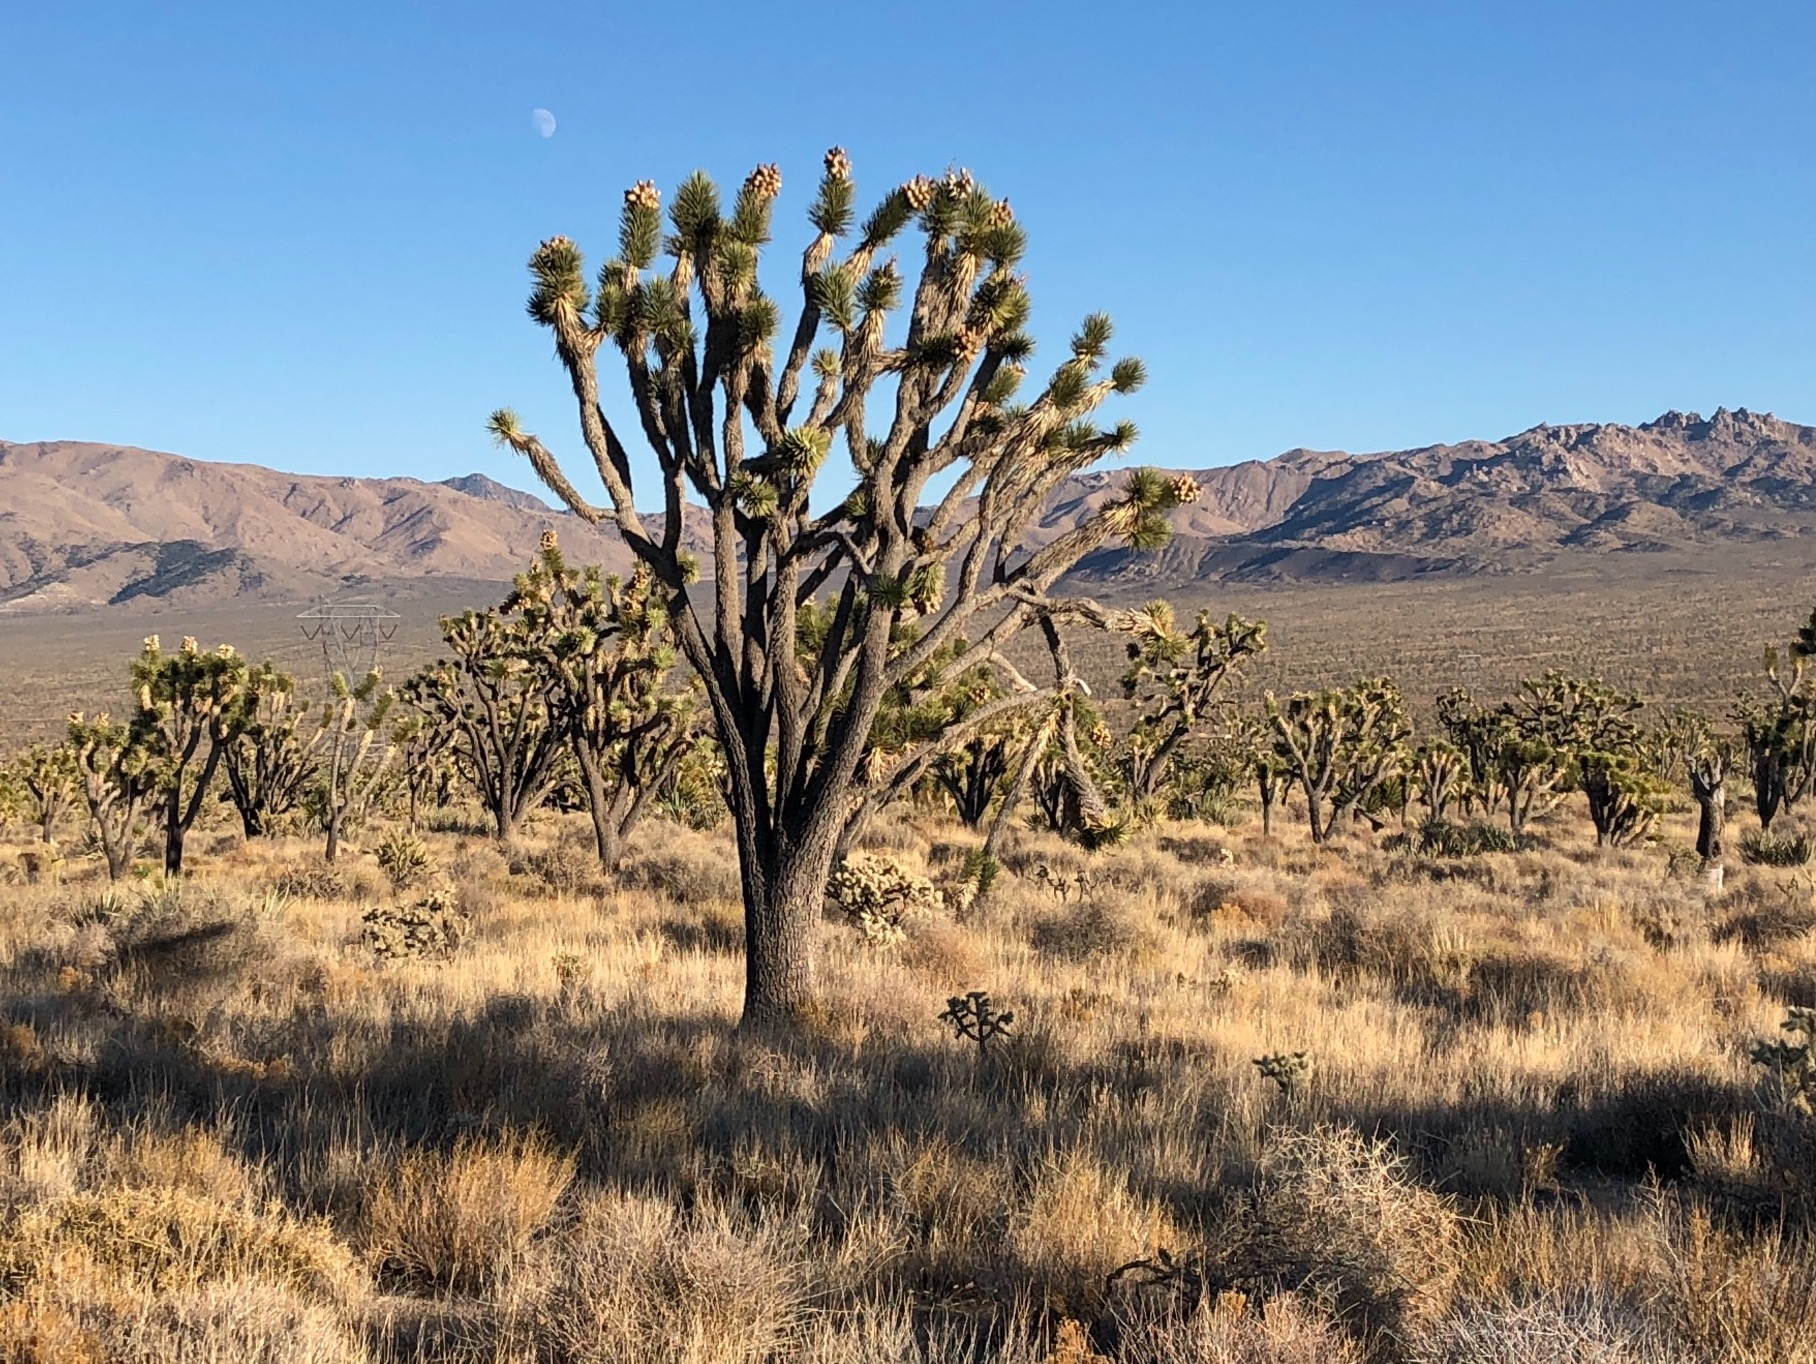
\includegraphics[width=1\linewidth]{images/cima2019}

East of Cima Dome in the Mojave National Preserve, California.
\textbf{Image Credit:} Center for Conservation Biology

\begin{center}
\includegraphics[width=0.75\linewidth]{images/ucrccb} \end{center}

\hypertarget{intro}{%
\chapter{Introduction}\label{intro}}

This Resource Guide provides an overview of the the UC Riverside Center for Conservation Biology (CCB) research team work processes and expectations. It hosts documentation on how to install software and project management tools utilized by the CCB team to facilitate collaborative research.

If you have suggestions for additions or changes, please make a pull request or contact Lynn Sweet (lynn.sweet AT ucr.edu).

\hypertarget{computer-requirements}{%
\section{Computer requirements}\label{computer-requirements}}

CCB work computers (laptop or desktop) operating systems should either be Windows or macOS. Please note that Windows based machine it required to run ESRI ArcDesktop and ArcPro software. Both Windows and macOS may utilize ESRI ArcOnline tools.

For \textbf{Mac} users, update macOS to the newest supported version. Navigate to System Preferences --\textgreater{} Software Update.

For \textbf{PC} users, ensure you have Windows 10 or 11 installed. If not, request a Windows key from UCR IT at \href{https://ucrsupport.service-now.com/ucr_portal?id=ucr_home}{UC Riverside ServiceLink}

\hypertarget{software-installation}{%
\section{Software Installation}\label{software-installation}}

Software installation covered in this resource guide includes:

\begin{itemize}
\tightlist
\item
  ESRI Platform

  \begin{itemize}
  \tightlist
  \item
    ArcGIS Desktop
  \item
    ArcGIS Pro
  \item
    ArcGIS Online
  \end{itemize}
\item
  git
\item
  GitHub
\item
  Google Apps
\item
  R
\item
  RStudio

  \begin{itemize}
  \tightlist
  \item
    Quarto
  \item
    Bookdown
  \end{itemize}
\item
  Slack
\item
  Trello
\item
  Zotero
\end{itemize}

\begin{center}\rule{0.5\linewidth}{0.5pt}\end{center}

Thank you to UC Santa Barbara's Bren School of Environmental Science \& Management and National Center for Ecological Analysis and Synthesis (NCEAS) staff for providing many of the resources listed in this reference guide. Information was made available on the \href{https://github.com/UCSB-MEDS}{UCSB-MEDS GitHub page}.

\hypertarget{r}{%
\chapter{R and RStudio Installation}\label{r}}

\hypertarget{install-r}{%
\section{Install R}\label{install-r}}

\textbf{R} is a programming language and environment used for statistical computing and grahics. For more information, please visit \href{https://www.r-project.org/about.html}{What is R}.

To install R, visit \href{https://cloud.r-project.org/}{cloud.r-project.org} to download the most recent version for your operating system.

Would you like a visual guide for install R and R Studio? Check out this YouTube R for Ecologist

\hypertarget{updating-r}{%
\subsection{Updating R}\label{updating-r}}

If you already have R installed, you may want to update the version of R you are using. Usually this occurs with a major version upgrades versus minor updates.

\textbf{Please be aware that when you update R, it means re-installing all of the packages you have previously installed.} It is worth updating R when major updates are released, especially if new packages you are attempting to install are not compatible with the version of R currently installed.

In order to update R, you have to find your installed version of R and run it on its own, outside of RStudio. This is easy if you have an R desktop shortcut, but not too hard if you hunt around a bit in your Applications folder.

\begin{flushleft}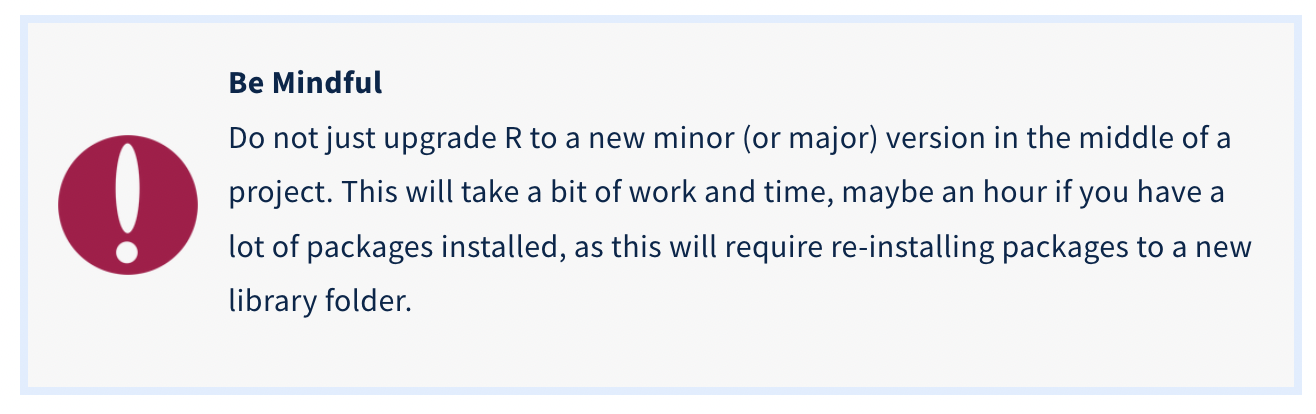
\includegraphics[width=1\linewidth]{images/rupdate} \end{flushleft}

\emph{Please see details below in Section 2.1.2 to save all R packages currently installed PRIOR to updating R, so you won't have to reinstall them individually after the update}

Double click the R icon to start up R. It will open the R Console and a menu. Click on the R menu at top left, and select Check for R Updates. If you are up to date, the R Console will report ``Your version of R is up to date''. If not, this process will provide windows and buttons to click to upgrade to the latest version of R. When done, quit R and start RStudio to make sure the update has carried over. You should see the new version number when RStudio starts.

\hypertarget{bulk-save-r-packages-prior-to-updates}{%
\subsection{Bulk Save R Packages Prior to Updates}\label{bulk-save-r-packages-prior-to-updates}}

In order to follow the bulk save R package instructions, you will need to have R Studio installed, and be familiar with the terminal and console panels.**

\begin{flushleft}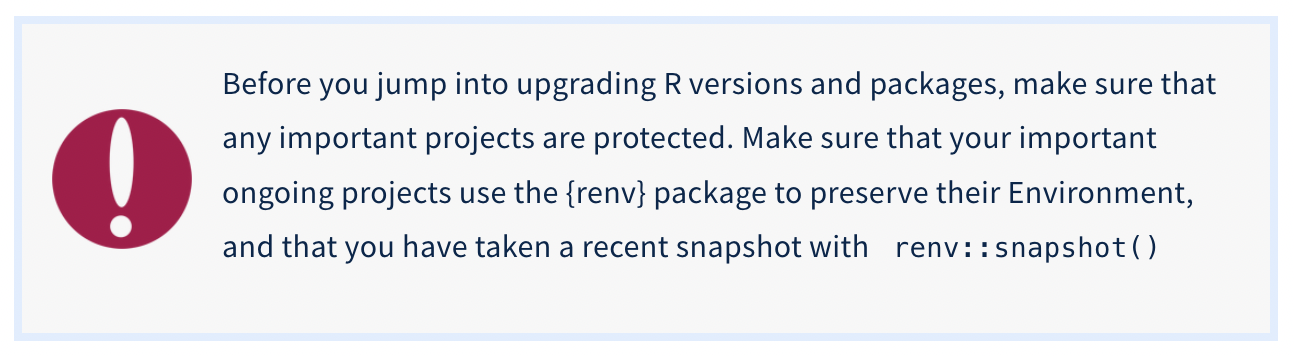
\includegraphics[width=1\linewidth]{images/renv} \end{flushleft}

Before updating R, check out where your current package library is saved by entering \texttt{.libPaths()} in the console of RStudio. This should look something like: \texttt{{[}1{]}\ "/Library/Frameworks/R.framework/Versions/4.2/Resources/library"}

Note that this package library is specific to the most recent major and minor version of R. If you upgrade from 4.1.x to 4.2.x, you will have a new library path to a new 4.2 folder, and will need to re-install packages in this folder.

You can do this from scratch, and install packages individually as needed (which is not a bad way to clean out packages you are not using), but you may prefer to re-install all packages in an organized way, rather than when you need to use one

You can see a dataframe of all currently installed packages by running the base R function \texttt{installed.packages()} in the R Studio console. This will help make a list of packages prior to updating R.

There is also a package for \textbf{Windows}, \{installr\}, which will pull the list of your current packages and install these in the correct folder for the new version of R. If you are on a Windows OS, and have installed the \{installr\} package, the \texttt{installr::updateR()} command in the console performs the following:

\begin{itemize}
\tightlist
\item
  finding the latest R version
\item
  downloading it
\item
  running the installer
\item
  deleting the installation file
\item
  copy old packages to the new R installation
\item
  updating old packages as needed for the new R installation
\end{itemize}

But for MacOS and UnixOS folks, this must be done manually.

\hypertarget{saving-a-list-of-r-packages-manually}{%
\subsubsection{Saving a List of R Packages Manually}\label{saving-a-list-of-r-packages-manually}}

The short script below will save a vector of your current packages to a file in your root (home) directory, named \texttt{installed.packages.rda}. Copy this code chunk below into your Console pane in RStudio and run it. Then reopen RStudio, go to the Files tab, click on Home , and check your root (home) directory for the installed.packages.rda file. You can click on this file to load it into your Environment tab (answer yes to load). In your Environment tab, it should look like a character vector with the names of all of your packages in quotes.

\begin{Shaded}
\begin{Highlighting}[]
\CommentTok{\# save list to tmp as a matrix object}
\NormalTok{tmp }\OtherTok{=} \FunctionTok{installed.packages}\NormalTok{()}

\CommentTok{\# filter for all rows where the \textquotesingle{}Priority\textquotesingle{} column is NA,}
\CommentTok{\# and select just (column 1) the package names in quotes,}
\CommentTok{\# and then assign this vector to the installedpackages}
\CommentTok{\# object}
\NormalTok{installedpackages }\OtherTok{=} \FunctionTok{as.vector}\NormalTok{(tmp[}\FunctionTok{is.na}\NormalTok{(tmp[, }\StringTok{"Priority"}\NormalTok{]), }\DecValTok{1}\NormalTok{])}

\CommentTok{\# save this vector as an *.rda file in your root (home)}
\CommentTok{\# directory}
\FunctionTok{save}\NormalTok{(installedpackages, }\AttributeTok{file =} \StringTok{"\textasciitilde{}/installed\_packages.rda"}\NormalTok{)}

\CommentTok{\# remove the tmp matrix and the installedpackages vector}
\CommentTok{\# from your Environment}
\FunctionTok{rm}\NormalTok{(tmp)}
\FunctionTok{rm}\NormalTok{(installedpackages)}
\end{Highlighting}
\end{Shaded}

Now that you have your saved list of packages stored in a file, you are ready to upgrade R. Quit RStudio, and go to \href{https://www.r-project.org/}{r-project.org}.

\hypertarget{reinstalling-list-of-r-packages}{%
\subsubsection{Reinstalling list of R Packages}\label{reinstalling-list-of-r-packages}}

First, let's check your new R version with \texttt{R.Version()} - run this in the Console pane. This should be the new version.

Now let's check your library path with \texttt{.libPaths()} - run this in the Console Pane - this should match your R version.

Now run \texttt{installed.packages()}. This should show that your new library is mostly empty, except for the base R packages. We will now fix that.

Now you need to take advantage of your nicely-stored list of packages to reinstall all of your packages in your new (mostly empty) library.

Use the short script below to load the file \texttt{installed.packages.rda} to open a vector of your previous packages in your Environment pane, and then re-install all of these packages. Copy the code chunk below into your Console pane in RStudio and run it. This will take a while, especially if you have a lot of packages installed.

While you are waiting, check out the code chunk below. The first step is to load the installedpackages.rda file from your root (home) directory into your Environment pane. Then it starts taking action on this vector of package names. See what it does in the next step, the for loop, and think about how it works. - It measures the length of the vector, installedpackages. - Then it counts from 1 to the length of installedpackages. - For each count, it installs the package at position {[}count{]} in the vector - Then it goes to the next {[}count{]} value, and installs the next package in the vector - Until it reaches the full length of the vector (installs the last package), and then stops.

\begin{Shaded}
\begin{Highlighting}[]
\CommentTok{\# loads vector into your Environment pane}
\FunctionTok{load}\NormalTok{(}\StringTok{"\textasciitilde{}/installed\_packages.rda"}\NormalTok{)}

\CommentTok{\# For each package in this vector of length [count],}
\CommentTok{\# install them one by one until the last one is installed.}

\ControlFlowTok{for}\NormalTok{ (count }\ControlFlowTok{in} \DecValTok{1}\SpecialCharTok{:}\FunctionTok{length}\NormalTok{(installedpackages)) \{}
    \FunctionTok{install.packages}\NormalTok{(installedpackages[count])}
\NormalTok{\}}
\end{Highlighting}
\end{Shaded}

When all of the installation is complete, you can check your work by running \texttt{installed.packages()} again in the R Studio console. You should see a full list of your packages, and you are updated and ready to go!

\hypertarget{install-or-update-r-studio}{%
\section{Install or Update R Studio}\label{install-or-update-r-studio}}

RStudio is a software (considered an Integrated Development Environment, or IDE) that provides R programmers with an easy-to-use interface for coding in R.

\textbf{Note:} RStudio will not work without R installed, and you won't particularly enjoy using R without having RStudio installed. Be sure to install both!

\begin{itemize}
\item
  \textbf{New install:} To install RStudio, visit \href{https://www.rstudio.com/products/rstudio/}{rstudio.com/products/rstudio/}. Download the free (``Open Source Edition'') Desktop version for your operating system.
\item
  \textbf{Update:} If you already have RStudio and need to update: Open RStudio, and under `Help' in the top menu, choose `Check for updates.' If you have the most recent release, it will return `No update available. You are running the most recent version of RStudio.' Otherwise, you should follow the instructions to install an updated version.
\end{itemize}

Open RStudio (logo you'll click on shown below). \textbf{If you are prompted to install Command Line Tools, do it.}

\begin{center}
\includegraphics[width=0.5\linewidth]{images/rstudio} \end{center}

\textbf{Mac Users}

There may be a need to install command line tools and \href{https://www.xquartz.org/}{XQuartz}:

\begin{itemize}
\item
  To install command line tools (if you're not automatically prompted), run in the Terminal tab in RStudio: \texttt{xcode-select\ -\/-install}
\item
  Visit \href{https://www.xquartz.org/}{xquartz.org} to download \& install XQuartz.
\end{itemize}

\hypertarget{update-r-packages-in-r-studio}{%
\subsection{Update R Packages in R Studio}\label{update-r-packages-in-r-studio}}

You will want to periodically update R packages to ensure you have the most up to date version. You can do this within RStudio by navigating via the Task Bar to \texttt{Tools/Check\ for\ Package\ Updates}.

\begin{itemize}
\tightlist
\item
  Select All, and let the updates begin.
\end{itemize}

\hypertarget{install-quarto}{%
\section{Install Quarto}\label{install-quarto}}

\emph{This is an optional tool within R Studio that is extremely powerful, but it is not required.}

Quarto is a scientific publishing tool built on Pandoc that allows R, Python, Julia, and ObservableJS users to create dynamic documents, websites, books and more.

As of \emph{July 2022}, Quarto comes pre-installed in R Studio (v2022.07). If you haven't updated your R Studio IDE (and concerned about doing so), you can install Quarto separately.

\begin{itemize}
\item
  Download Quarto \href{https://quarto.org/docs/get-started/}{here} and install
\item
  To use Quarto through the RStudio IDE, be sure to have at least version v2022.02 installed (see directions in step 2, above)
\end{itemize}

Learn more about Quarto \href{https://quarto.org/docs/get-started/hello/rstudio.html}{here}.

\hypertarget{learn-how-to-use-r-rstudio}{%
\section{Learn How to Use R \& RStudio}\label{learn-how-to-use-r-rstudio}}

There are many resources out there to help you learn how to use R and the RStudio IDE (YouTube, Googling, \href{https://stackoverflow.com/}{StackOverflow}, etc\ldots). This is a short list of primary resources for you to reference. We encourage you to join R community Slack workspaces, R User community groups (such as \href{https://rladies.org/}{R-Ladies}), and UC Riverside Data Science clubs!

\begin{itemize}
\tightlist
\item
  \href{https://acmucr.org/index.html}{ACM at UCR} - UC Riverside community dedicated to technical, professional, and personal development in the context of computer science.
\item
  \href{https://r4ds.had.co.nz/}{R for Data Science}
\item
  \href{https://bookdown.org/yihui/rmarkdown-cookbook/}{R Markdown Cookbook}
\item
  \href{http://www.cookbook-r.com/}{Cookbook for R}
\item
  \href{https://adv-r.hadley.nz/}{Advanced R}
\item
  \href{https://www.rstudio.com/resources/books/}{R Studio (posit) Book Catalog}
\item
  \href{https://www.rfordatasci.com/}{R for Data Science Online Learning Community}
\item
  \href{https://ropensci.org/}{R OpenSci}
\item
  \href{https://rstudio.cloud/learn/primers}{RStudio Cloud} - interactive tutorials to learn data science basics.
\item
  \href{https://www.rstudio.com/resources/cheatsheets/}{R Studio Cheatsheets} - invaluable tool to learn how to use various R packages.
\item
  \href{https://swirlstats.com/}{Swirl} - R package that is a built in tutorial.
\item
  \href{https://tinystats.github.io/teacups-giraffes-and-statistics/index.html}{Teacups, Giraffes, \& Statistics} - an interactive tutorial to learn statistics and R coding, plus it is a beautiful!
\item
  \href{https://datasciencebox.org/}{Data Science in a Box}
\item
  \href{https://www.adventures-in-r.com/}{Adventures in R}
\item
  \href{https://datacarpentry.org/R-ecology-lesson/}{Data Analysis \& Visualization in R for Ecologist}
\end{itemize}

\hypertarget{bookdown}{%
\chapter{Bookdown Guide}\label{bookdown}}

This Resource Guide was created using the \href{https://github.com/rstudio/bookdown}{\texttt{bookdown}} package. \textbf{bookdown} provides a platform to publish references using various output formats (PDF, HTML, Word) and allows for interactivity, insertion of code chunks, and supports a variety of languages (R, Python, Julia, SQL, etc.).

\hypertarget{primary-reference-resources}{%
\section{Primary Reference Resources}\label{primary-reference-resources}}

Here is a list of resources to learn how to use and edit in bookdown

\begin{itemize}
\tightlist
\item
  \href{https://bookdown.org/}{Bookdown Package Documentation}
\item
  \href{https://bookdown.org/yihui/bookdown/}{Authoring Books with R Markdown}
\item
  \href{https://bookdown.org/yihui/rmarkdown-cookbook/}{R Markdown Cookbook}
\item
  \href{https://bookdown.org/yihui/rmarkdown/}{R Markdown: The Definitive Guide}
\end{itemize}

\hypertarget{install-the-bookdown-package}{%
\section{Install the Bookdown package}\label{install-the-bookdown-package}}

The first step to edit and add to this Resource Guide is to install the \textbf{bookdown} package from CRAN or Github. In the RStudio console, run the following:

\begin{Shaded}
\begin{Highlighting}[]
\FunctionTok{install.packages}\NormalTok{(}\StringTok{"bookdown"}\NormalTok{)}
\CommentTok{\# or the development version}
\CommentTok{\# devtools::install\_github(\textquotesingle{}rstudio/bookdown\textquotesingle{})}
\end{Highlighting}
\end{Shaded}

\hypertarget{additional-packages}{%
\subsection{Additional packages}\label{additional-packages}}

You may need to install additional packages if you do not currently have them in order to render the Resource Guide bookdown:

\begin{itemize}
\tightlist
\item
  \texttt{formatR}
\item
  \texttt{here}
\item
  \texttt{kableExtra}
\item
  \texttt{Rtools}
\item
  \texttt{shiny}
\item
  \texttt{tidyverse}
\end{itemize}

\hypertarget{install-tinytex}{%
\subsection{Install TinyTex}\label{install-tinytex}}

TinyTeX is a custom LaTeX distribution. LaTeX, which is pronounced «Lah-tech» or «Lay-tech», is a document preparation system for high-quality typesetting. It is most often used for technical or scientific documents. To learn more about TinyTex, \href{https://yihui.org/tinytex/}{navigate to this document}, and to learn more about LaTex, \href{https://www.latex-project.org/}{visit the LaTex Project site}.

To install TinyTex on your computer, navigate to the R Studio console panel, and type in the following command:

\texttt{tinytex::install\_tinytex()}

\hypertarget{render-build-publish-the-resource-guide}{%
\section{Render, Build \& Publish the Resource Guide}\label{render-build-publish-the-resource-guide}}

When updates are made to the Resource Guide, it needs to be rendered, built, and then the updates published.

In your Console, type either of these commands depending on which type of render you prefer:

\texttt{bookdown::render\_book("index.Rmd",\ "bookdown::gitbook")}
\texttt{bookdown::render\_book("index.Rmd",\ "bookdown::pdf\_book")}

\textbf{Note:} If there is an error during rendering, Google what the error message means! You should be able to find an answer on \href{https://stackoverflow.com/}{stack overflow} or other tech support site. One of the most common errors during rendering is that not all dependencies (aka packages) have been installed on your local computer.

\begin{figure}

{\centering 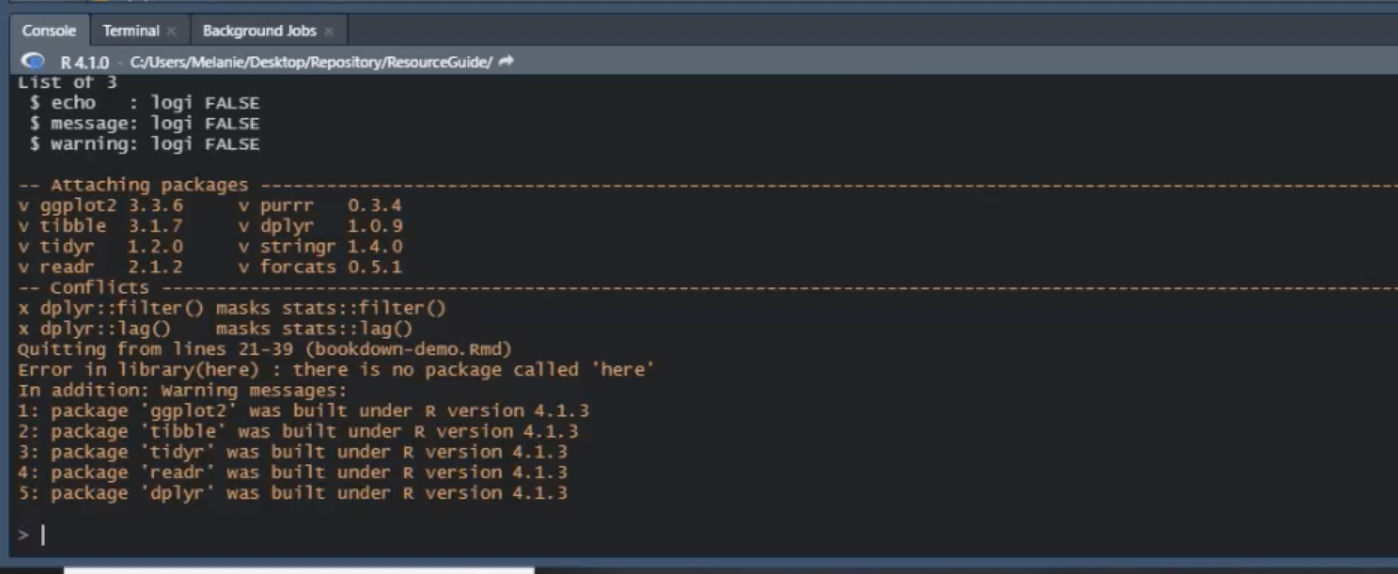
\includegraphics[width=0.95\linewidth]{images/bookdown_here} 

}

\caption{An common error message in the RStudio console: Error in library(here): there is no package called `here`. If you see this library error message, all you need to do is install the required package! The additional warning messages are notifications that R should be updated to be compatiable with the current packages. These will not hender the render.}\label{fig:rendererror}
\end{figure}

Once you have rendered updates using the console commands above:

\begin{itemize}
\tightlist
\item
  navigate to the \textbf{Environment, Connections, Build, Git} panel,
\item
  select the \textbf{Build} tab,
\item
  select \textbf{Build Bookdown}
\item
  once the build is complete (the final line should read \texttt{Output\ created:\ docs/index/html}), commit, pull and push updates to GitHub via the \textbf{Git} tab.
\end{itemize}

\begin{center}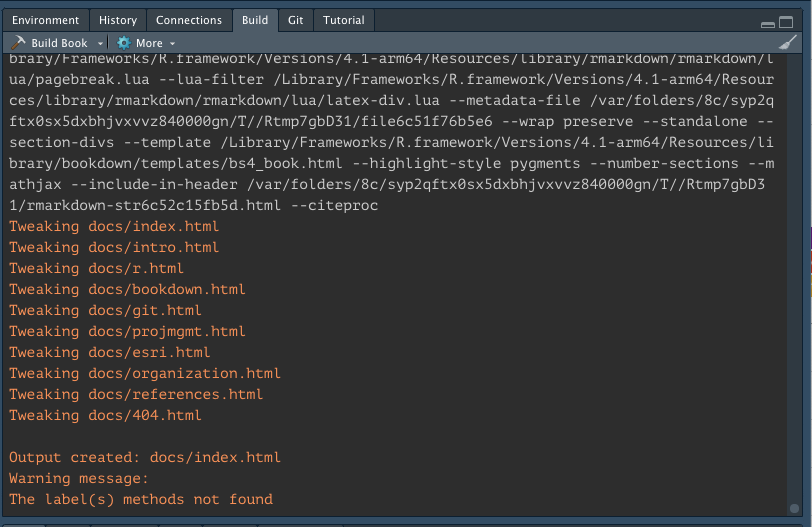
\includegraphics[width=0.75\linewidth]{images/build} \end{center}

\begin{center}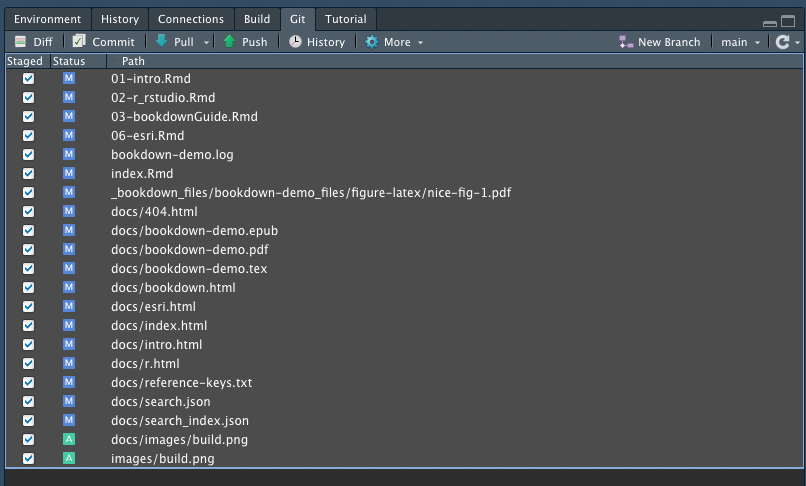
\includegraphics[width=0.75\linewidth]{images/select} \end{center}

\begin{center}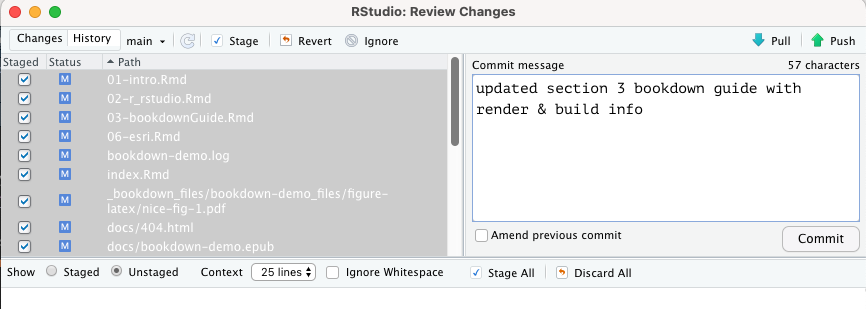
\includegraphics[width=0.75\linewidth]{images/commit} \end{center}

\begin{center}\rule{0.5\linewidth}{0.5pt}\end{center}

\textbf{The following information is directly taken from the \emph{bookdown} package} \citep{R-bookdown}.

\hypertarget{formatting}{%
\section{Formatting}\label{formatting}}

You can use anything that Pandoc's Markdown supports, e.g., a math equation \(a^2 + b^2 = c^2\).

\hypertarget{referencing-bookdown-chapters}{%
\subsection{Referencing Bookdown Chapters}\label{referencing-bookdown-chapters}}

Remember each Rmd file contains one and only one chapter, and \textbf{a chapter} is defined by the first-level heading \texttt{\#}.

You can label chapter and section titles using \texttt{\{\#label\}} after them, e.g., reference this Resource Guide Chapter \ref{intro} by using the markdown format: \texttt{\textbackslash{}@ref(insert\ chapter\ label\ name\ here)}. If you do not manually label them, there will be automatic labels anyway, e.g., Chapter \ref{methods}.

\hypertarget{formatting-figures}{%
\subsection{Formatting Figures}\label{formatting-figures}}

Figures and tables with captions will be placed in \texttt{figure} and \texttt{table} environments, respectively.

\begin{figure}

{\centering 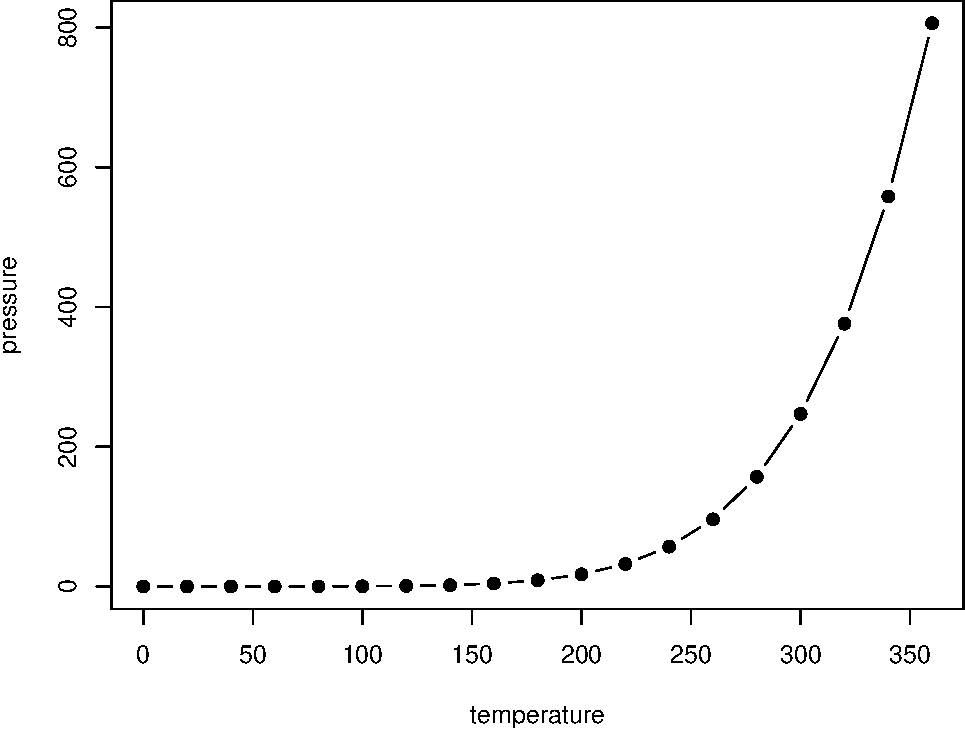
\includegraphics[width=0.8\linewidth]{bookdown-demo_files/figure-latex/nice-fig-1} 

}

\caption{Here is a nice figure!}\label{fig:nice-fig}
\end{figure}

Reference a figure by its code chunk label with the \texttt{fig:} prefix, e.g., see Figure \ref{fig:nice-fig}. Similarly, you can reference tables generated from \texttt{knitr::kable()}, e.g., see Table \ref{tab:nice-tab}.

\begin{table}

\caption{\label{tab:nice-tab}Here is a nice table!}
\centering
\begin{tabular}[t]{rrrrl}
\toprule
Sepal.Length & Sepal.Width & Petal.Length & Petal.Width & Species\\
\midrule
5.1 & 3.5 & 1.4 & 0.2 & setosa\\
4.9 & 3.0 & 1.4 & 0.2 & setosa\\
4.7 & 3.2 & 1.3 & 0.2 & setosa\\
4.6 & 3.1 & 1.5 & 0.2 & setosa\\
5.0 & 3.6 & 1.4 & 0.2 & setosa\\
\addlinespace
5.4 & 3.9 & 1.7 & 0.4 & setosa\\
4.6 & 3.4 & 1.4 & 0.3 & setosa\\
5.0 & 3.4 & 1.5 & 0.2 & setosa\\
4.4 & 2.9 & 1.4 & 0.2 & setosa\\
4.9 & 3.1 & 1.5 & 0.1 & setosa\\
\addlinespace
5.4 & 3.7 & 1.5 & 0.2 & setosa\\
4.8 & 3.4 & 1.6 & 0.2 & setosa\\
4.8 & 3.0 & 1.4 & 0.1 & setosa\\
4.3 & 3.0 & 1.1 & 0.1 & setosa\\
5.8 & 4.0 & 1.2 & 0.2 & setosa\\
\addlinespace
5.7 & 4.4 & 1.5 & 0.4 & setosa\\
5.4 & 3.9 & 1.3 & 0.4 & setosa\\
5.1 & 3.5 & 1.4 & 0.3 & setosa\\
5.7 & 3.8 & 1.7 & 0.3 & setosa\\
5.1 & 3.8 & 1.5 & 0.3 & setosa\\
\bottomrule
\end{tabular}
\end{table}

\hypertarget{citations}{%
\subsection{Citations}\label{citations}}

You can easily write citations using .bib files within this repository formatted using \href{http://www.bibtex.org/}{BibTEX}. For example, the \textbf{bookdown} package \citep{R-bookdown} in this reference book, which was built on top of R Markdown and \textbf{knitr} \citep{xie2015}.

\hypertarget{alt-text-for-accessibility}{%
\subsection{Alt Text for Accessibility}\label{alt-text-for-accessibility}}

\href{https://www.rstudio.com/blog/knitr-fig-alt/}{Use the knitr package to add alt text to graphics in R Markdown files}

\hypertarget{migrating-to-quarto-from-bookdown}{%
\subsection{Migrating to Quarto from Bookdown}\label{migrating-to-quarto-from-bookdown}}

Love \texttt{bookdown}? Check out \texttt{Quarto}! To learn how to convert \texttt{bookdown} documents to \texttt{Quarto}, check out this blogpost on \href{https://www.openscapes.org/blog/2022/07/21/quarto-migrate/}{Openscapes}

\hypertarget{git}{%
\chapter{Git Installation \& GitHub Account}\label{git}}

\hypertarget{github}{%
\section{GitHub}\label{github}}

GitHub is a internet based code hosting platform for collaboration and \href{https://www.atlassian.com/git/tutorials/what-is-version-control\#:~:text=Version\%20control\%2C\%20also\%20known\%20as,to\%20source\%20code\%20over\%20time.}{version control}. GitHub lets you (and others) work together on projects.

Navigate to \href{https://github.com/}{github.com}, and create an account! Please use either your work or personal email account. You can add several emails to your account, and assign a particular email as the primary email for the account.

Review this article on choosing a GitHub username: \url{happygitwithr.com/github-acct.html}.

Once you have created a GitHub account, join the \href{https://github.com/ccbucr}{CCB's GitHub Organization}. Please email the CCB PI to request they invite you to the organization.

\hypertarget{git-1}{%
\section{Git}\label{git-1}}

Git is a tool utilized for source code management. It tracks changes and updates to code and allows for multiple users to work together within the same repository. Recommended reading for \href{https://towardsdatascience.com/what-is-git-and-why-is-it-so-important-dce559b27833}{background information on Git and its utility} \citep{Yıldırım_2020}.

Check to see if your computer already has git:

\begin{enumerate}
\def\labelenumi{\arabic{enumi}.}
\tightlist
\item
  Open RStudio
\item
  In the terminal, run the following command:
\end{enumerate}

\begin{itemize}
\tightlist
\item
  \texttt{which\ git} (Mac, Linux)
\item
  \texttt{where\ git} (Windows)
\end{itemize}

If \texttt{git} is already installed, the return to the above command should return a filepath similar to:

\begin{itemize}
\tightlist
\item
  MacOS \texttt{/usr/local/bin/git}
\item
  Windows \texttt{C:/Program\ Files/Git/bin/git.exe}
\end{itemize}

\begin{enumerate}
\def\labelenumi{\arabic{enumi}.}
\setcounter{enumi}{2}
\tightlist
\item
  If there is no response, download and install \texttt{git} from here: \href{https://git-scm.com/downloads}{git-scm.com/downloads}. Select the default settings within the prompts \textbf{except} the default to \textbf{master} branch. This branch is being phased out, so select the option that let's you select alternative branches (ex: main).
\end{enumerate}

Once Git is installed and your GitHub account has been set up, Git needs to be configured on the computer. Configuring Git is required to push \& pull commits to GitHub.

Configuring Git:

\begin{enumerate}
\def\labelenumi{\arabic{enumi}.}
\tightlist
\item
  In RStudio, open the terminal.
\item
  Run the following commands separately, pressing \texttt{Enter} after each line. Replace username and email with your GitHub account username and email. Make sure to keep the quotes around the username in the code below:
\end{enumerate}

\begin{itemize}
\tightlist
\item
  \texttt{git\ config\ -\/-global\ user.name\ "Jane\ Doe"}
\item
  \texttt{git\ config\ -\/-global\ user.email\ janedoe@example.com}
\end{itemize}

\begin{enumerate}
\def\labelenumi{\arabic{enumi}.}
\setcounter{enumi}{2}
\tightlist
\item
  Once you have entered the above command line code, check that the configuration was set correctly. In the RStudio Terminal, type the following command and hit enter:
\end{enumerate}

\begin{itemize}
\tightlist
\item
  \texttt{git\ config\ -\/-list\ -\/-global}
\end{itemize}

In the terminal, it should show code similar to this in the Terminal:

\texttt{user.name=janedoe}
\texttt{user.email=janedoe@ucr.edu}
\texttt{core.excludesfile=/Users/janedoe/.gitignore}

If when installing or updating Git, the default branch was not set to \texttt{main} (it is defaulting to the old \texttt{master} branch), you can change this setting globally. In the Terminal again, enter the line below:

\texttt{git\ config\ -\/-global\ init.defaultBranch\ main}

For more information on configuring Git: \href{https://git-scm.com/book/en/v2/Getting-Started-First-Time-Git-Setup}{check out this Git reference}

\hypertarget{personal-access-token}{%
\section{Personal Access Token}\label{personal-access-token}}

Once Git has been configured to commit to your GitHub account, a \textbf{Personal Access Token (PAT)} must be created for \textbf{each computer you intend to use}. A PAT is an alternative password authentication method for Git to access GitHub accounts.

\begin{itemize}
\tightlist
\item
  In the RStudio Console, install the \href{https://usethis.r-lib.org/}{\texttt{usethis}} package in R by running the following code:
\end{itemize}

\texttt{install.packages("usethis")}

If the \texttt{usethis} package is installed correctly, at the end of the stream of text there should be a message similar to the image below:

\begin{flushleft}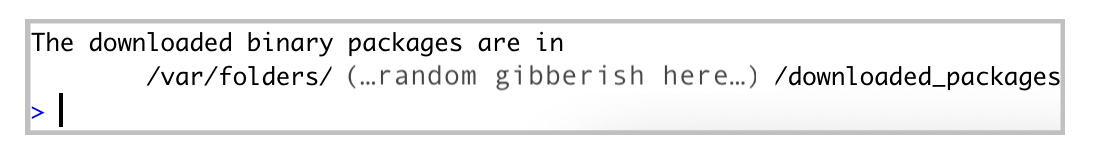
\includegraphics[width=0.8\linewidth]{images/usethis} \end{flushleft}

\begin{itemize}
\tightlist
\item
  Once the \texttt{usethis} package is installed, run the following in the RStudio Console:
\end{itemize}

\texttt{usethis::create\_github\_token()}

\begin{itemize}
\tightlist
\item
  Enter your GitHub password when prompted.
\end{itemize}

This should take you to the \textbf{Settings/Developer settings} section of your GitHub account:

\begin{flushleft}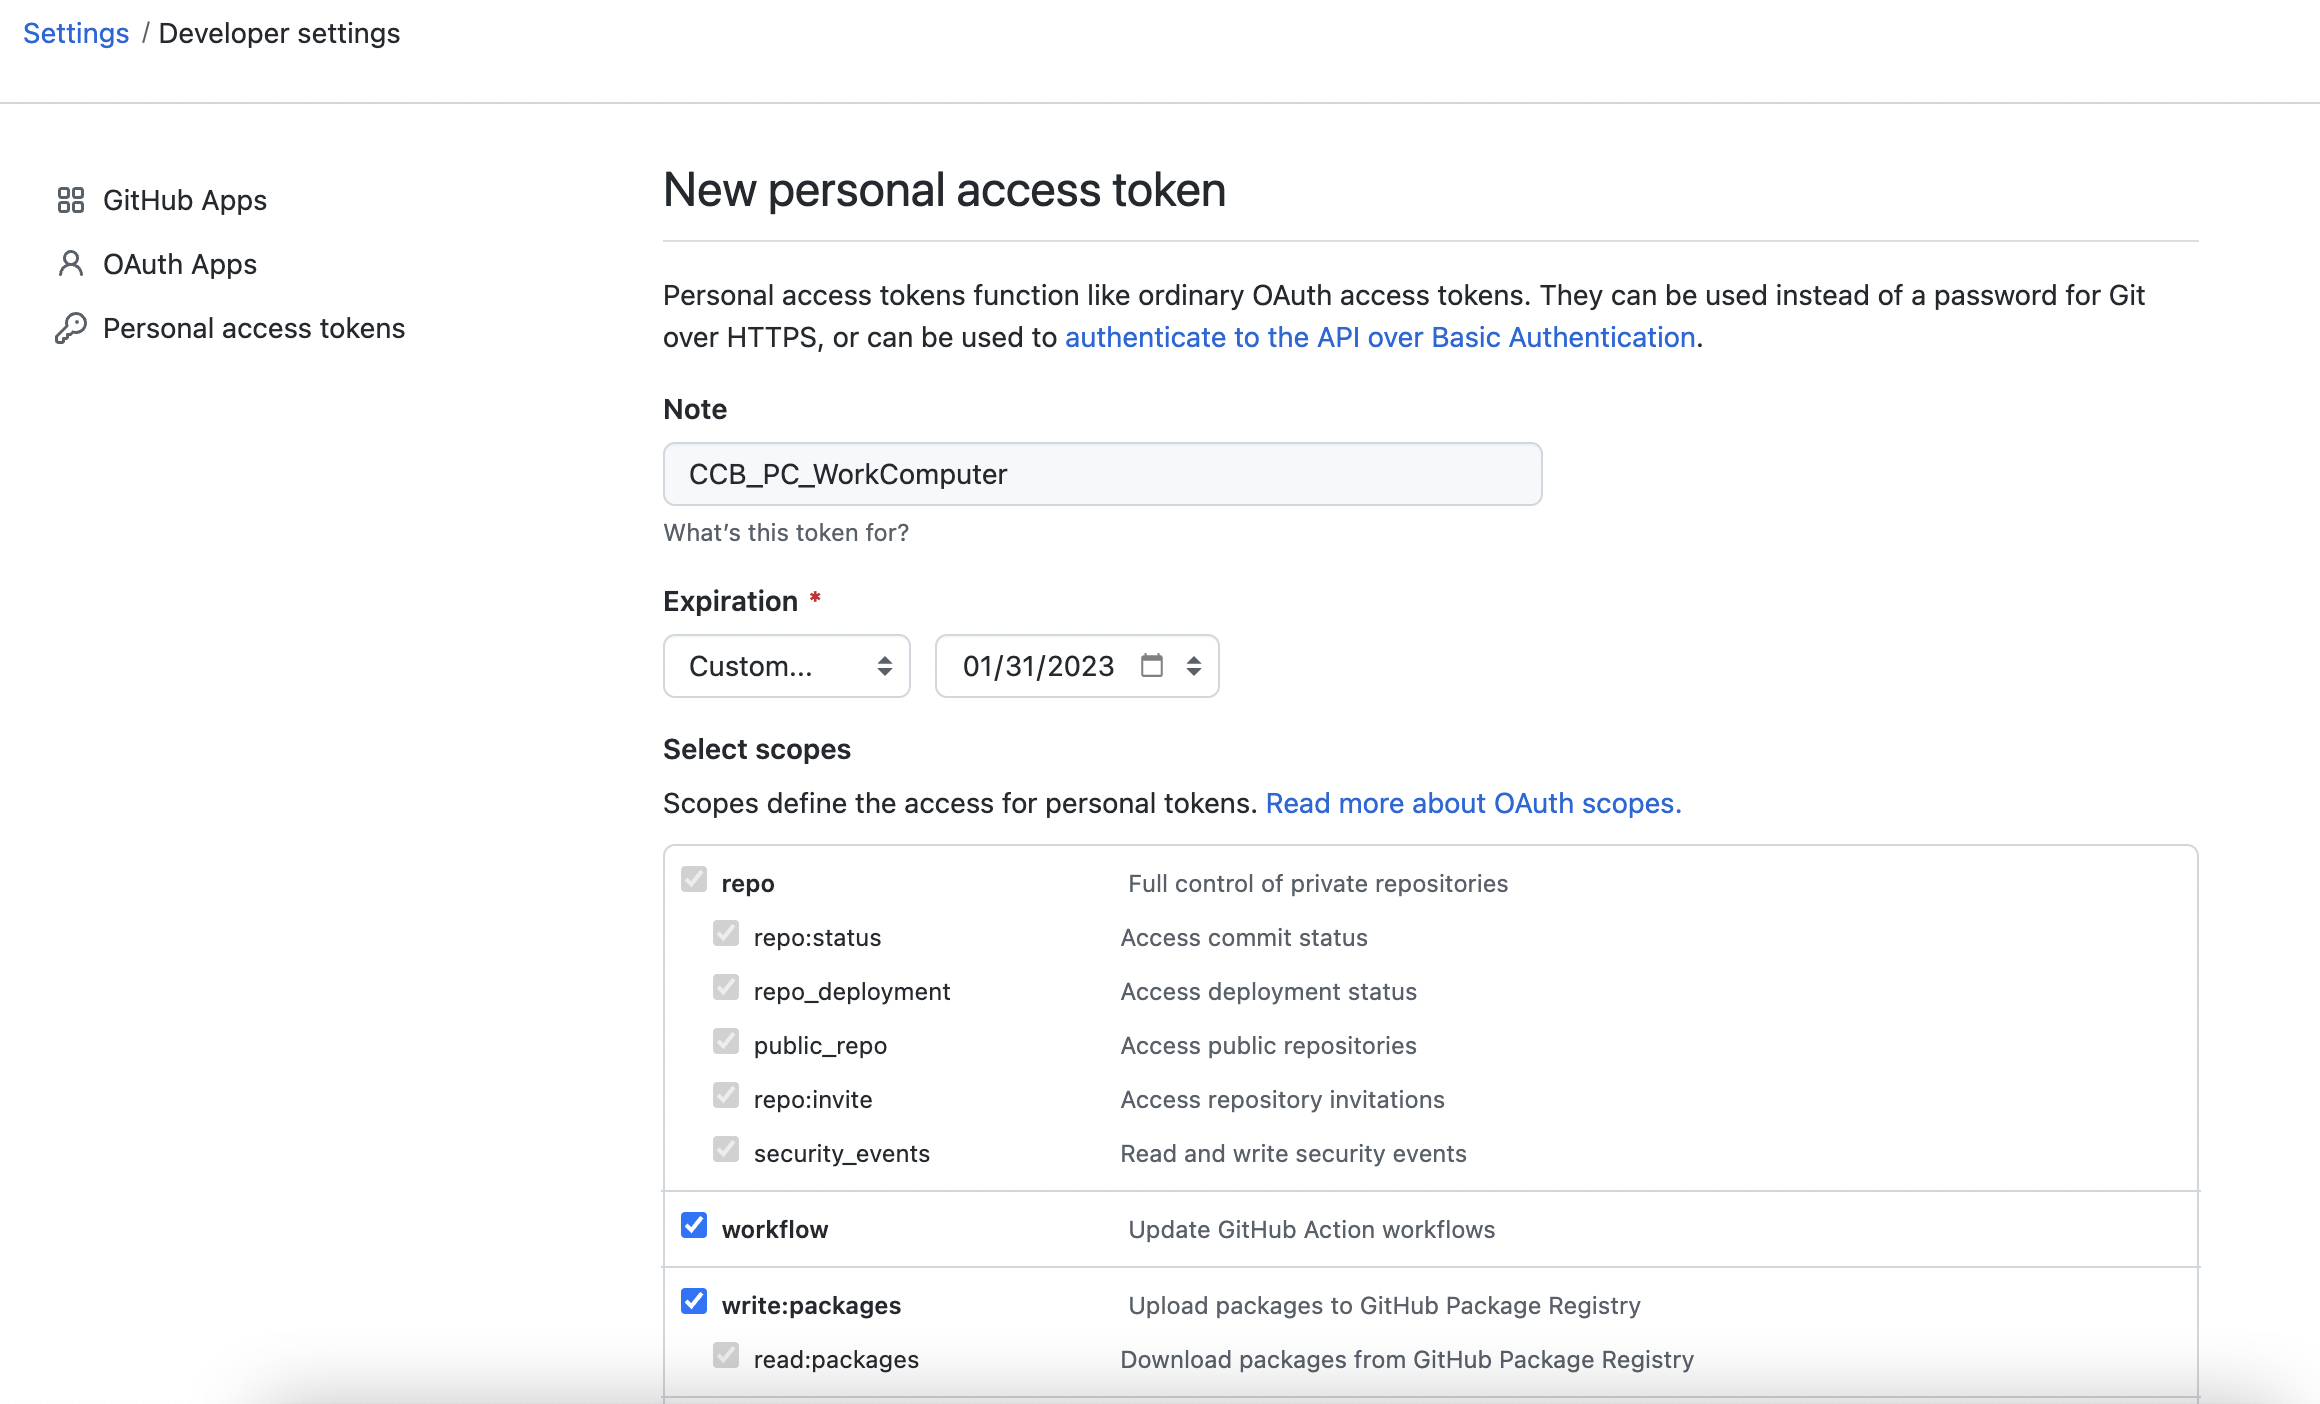
\includegraphics[width=0.8\linewidth]{images/pat} \end{flushleft}

\begin{itemize}
\tightlist
\item
  \textbf{Note Field}
\end{itemize}

Change the PAT name to a meaningful reference (see image for an example). You may end up creating multiple PATs, so you want to ensure that you know which PAT is designated for each computer \textbar{} server.

\begin{itemize}
\tightlist
\item
  \textbf{Expiration Field}
\end{itemize}

This is to select a set expiration timeframe for your PAT. Setting an expiration is highly recommended, and GitHub will send you \emph{SEVERAL} emails prior to it expiring to remind you to renew it. Use the drop down to select a set time frame (7 days to 90 days) or create a custom expiration time frame (exactly a year or particular date).

\begin{itemize}
\tightlist
\item
  \textbf{Select Scopes Field}
\end{itemize}

Define access for the Personal Access Token being generated.

It is recommended to select at least the following scopes:
- repo
- workflow
- write:packages
- notifications
- delete repo
- write:discussions
- project

To learn more about Scopes, visit \href{https://docs.github.com/en/developers/apps/building-oauth-apps/scopes-for-oauth-apps}{the GitHub Scopes for OAUth Apps page}.

\begin{itemize}
\tightlist
\item
  Once Scopes are selected, click on the green \texttt{Generate\ token} button:
\end{itemize}

\begin{center}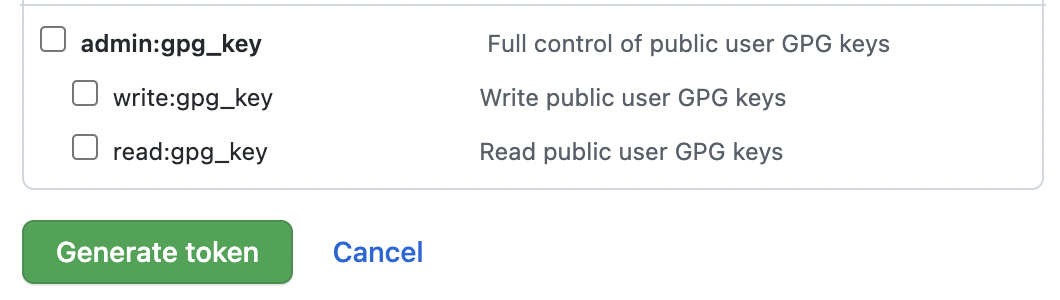
\includegraphics[width=0.8\linewidth]{images/generatepat} \end{center}

\begin{itemize}
\item
  Copy the generated PAT to your clipboard.
\item
  Paste and Save this PAT in a text file in a secure folder that will NEVER be accessed by other users or the internet. You can create a \texttt{private} folder on your personal computer to store these files.
\item
  Return to RStudio Console and run the following command:
\end{itemize}

\texttt{gitcreds::gitcreds\_set()}.

You will be prompted to paste the PAT into the console:

\begin{center}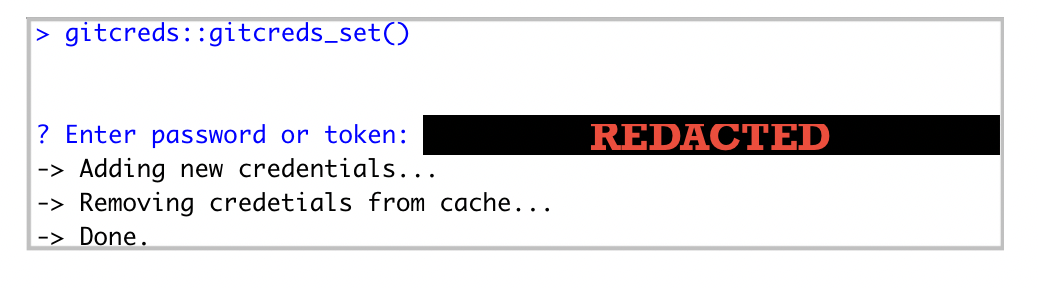
\includegraphics[width=0.8\linewidth]{images/paste_pat} \end{center}

Paste the PAT at the end of the line \texttt{Enter\ password\ or\ token:} and press enter.

\begin{itemize}
\tightlist
\item
  In the console, run:
\end{itemize}

\texttt{usethis::git\_sitrep()}

This command should return your GitHub account information (see example below).

\begin{center}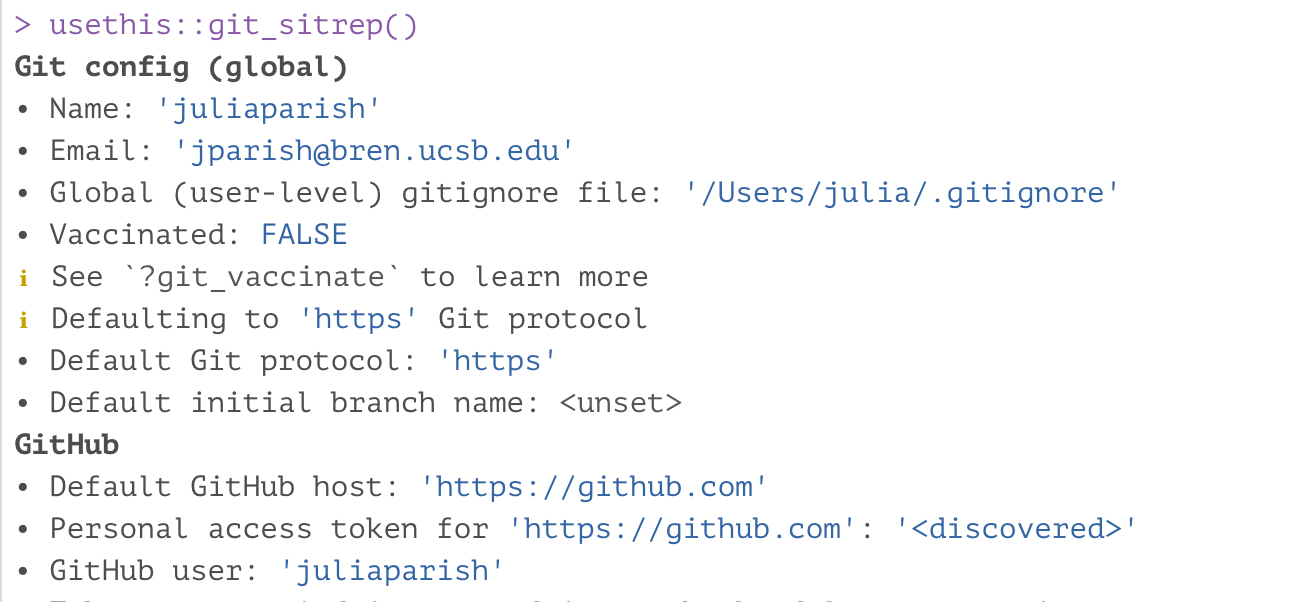
\includegraphics[width=0.8\linewidth]{images/gitsitrep} \end{center}

For more information on PATs, check out \href{https://docs.github.com/en/authentication/keeping-your-account-and-data-secure/creating-a-personal-access-token}{GitHub's PAT information page}.

\hypertarget{projmgmt}{%
\chapter{Project Management Tools}\label{projmgmt}}

\hypertarget{ucr-vpn---globalprotect}{%
\section{UCR VPN - GlobalProtect}\label{ucr-vpn---globalprotect}}

UC Riverside provides free access to a Virtual Private Network (VPN), GlobalProtect, that allows you to access the CCB NAS Server or campus resources (ex: library services) when working remotely.

To install and use the GlobalProtect VPN, navigate to the UCR ServiceLink \href{https://ucrsupport.service-now.com/ucr_portal/?id=kb_article\&sys_id=8a264d791b5f0c149c0b844fdd4bcb34}{GlobalProtect Connection Installation Instructions}.

\hypertarget{ccb-nas-server}{%
\section{CCB NAS Server}\label{ccb-nas-server}}

The Center for Conservation Biology has a NAS Server, which serves as the primary data storage location to access data and reference files. CCB staff should ensure that all work and research related files are saved on the NAS. Reference \textbf{Chapter} \ref{organization} for proper directory organization and file naming.

Network-attached storage (NAS) is dedicated file storage that enables multiple users to retrieve data from centralized disk capacity. The purpose of NAS is to enable users to collaborate and share data more effectively. It is especially useful to teams that need remote access. NAS connects to a wireless router, making it easy for remote workers to access files from any device with a network connection.

The CCB NAS server model is Synology DS920+. For more information on the unit, see \textbf{Chapter} \ref{equipment}.

\hypertarget{access-the-ccb-nas-server-from-local-computer}{%
\subsection{Access the CCB NAS Server from Local Computer}\label{access-the-ccb-nas-server-from-local-computer}}

In order to access the CCB NAS, there just a few steps:

\begin{itemize}
\item
  \textbf{Step 01:} Request the creation of a NAS user account through the designated CCB staff member. You will need to provide your preferred \textbf{username} (typically similar to UCR ID) and a \textbf{passcode}. The passcode must be a strong code: a unique code with 12 - 15 characters consisting of a mix of letters, numbers, symbols, and does not contain personal information.
\item
  \textbf{Step 02:} Once a user account has been created, log onto the UCR VPN (\emph{see above section}).
\item
  \textbf{Step 03:} Map the server onto your local computer:

  \begin{itemize}
  \tightlist
  \item
    For PCs running Windows 11:

    \begin{enumerate}
    \def\labelenumi{\arabic{enumi}.}
    \tightlist
    \item
      Open File Explorer on Windows 11.
    \item
      Click on \texttt{This\ PC} from the left pane.
    \item
      Click the \texttt{See\ More} (three-dotted) button in the command bar and select the ``Map network drive'' option.
    \end{enumerate}
  \end{itemize}
\end{itemize}

\begin{flushleft}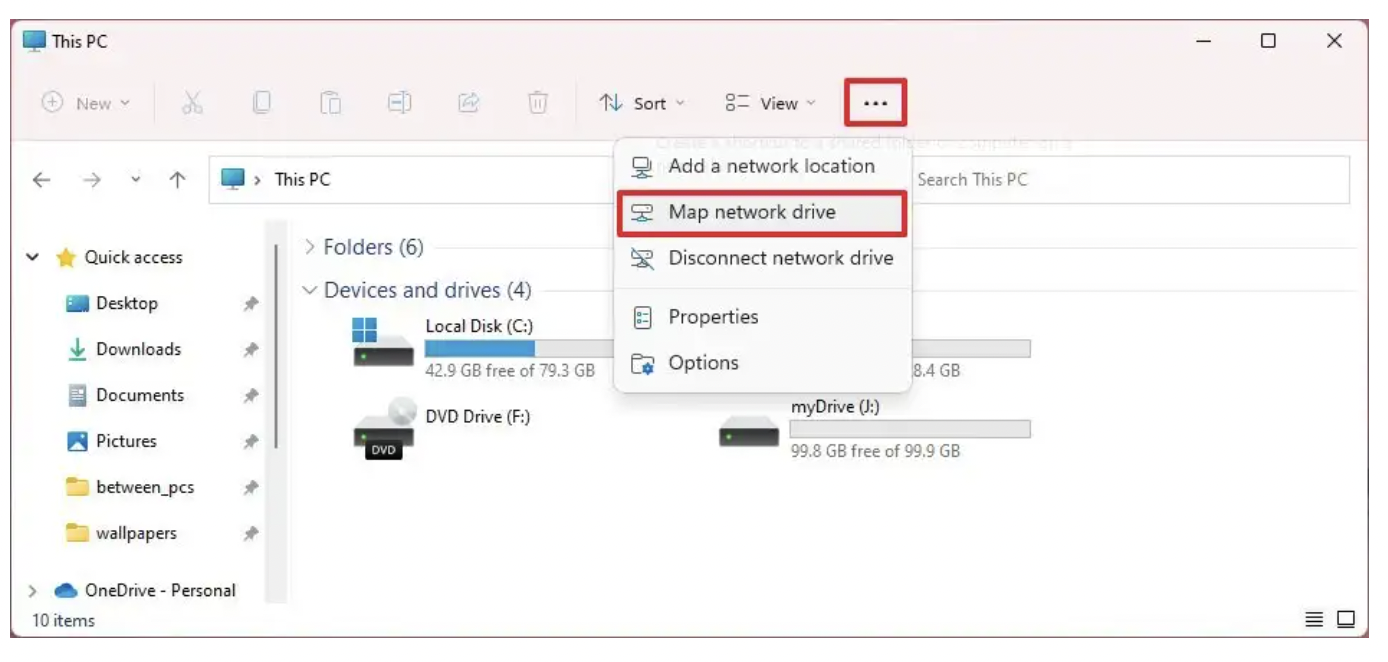
\includegraphics[width=0.8\linewidth]{images/nas_map} \end{flushleft}

\begin{enumerate}
\def\labelenumi{\arabic{enumi}.}
\setcounter{enumi}{3}
\tightlist
\item
  Use the \texttt{Drive} drop-down menu and choose a letter to assign the drive.

  \begin{enumerate}
  \def\labelenumii{\arabic{enumii}.}
  \setcounter{enumii}{4}
  \tightlist
  \item
    In the \texttt{Folder} field, enter the network path to the shared folder, \texttt{\textbackslash{}\textbackslash{}CCBNAS.dyn.ucr.edu\textbackslash{}pdo}. (Or click the Browse button to browse the folder to map as a network drive, and click the OK button.)
  \end{enumerate}
\end{enumerate}

\begin{flushleft}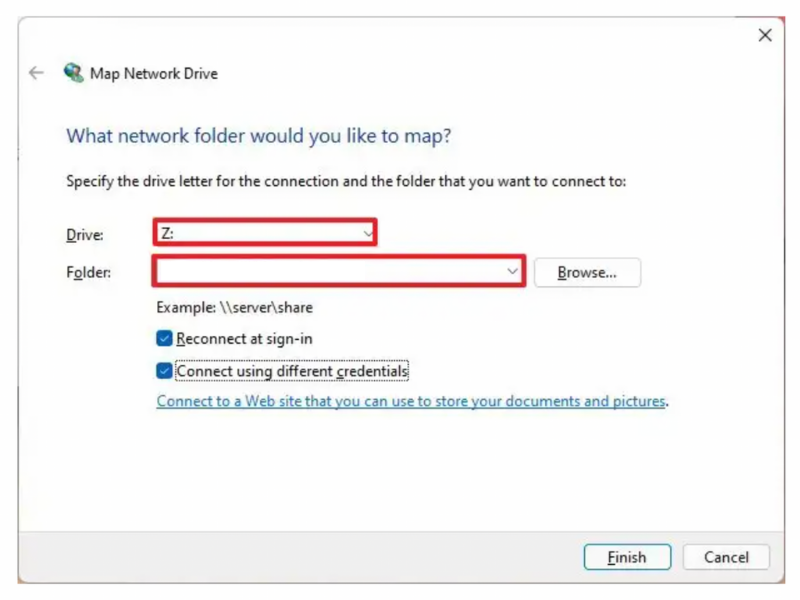
\includegraphics[width=0.75\linewidth]{images/nas_path} \end{flushleft}

\begin{enumerate}
\def\labelenumi{\arabic{enumi}.}
\setcounter{enumi}{5}
\tightlist
\item
  Check the \texttt{Reconnect\ at\ sign-in} option to make the connection permanent.

  \begin{enumerate}
  \def\labelenumii{\arabic{enumii}.}
  \setcounter{enumii}{6}
  \tightlist
  \item
    Check the Connect using different credentials option if the credentials are different from the account you are already using.
  \item
    Click the Finish button.
  \item
    Confirm the network account credentials (if applicable) to map the network drive to Windows 11.
  \item
    Click the OK button.
  \end{enumerate}
\end{enumerate}

Once you complete the steps, the network drive will become available in File Explorer.

If you run into issues, first read over this \href{https://www.robertwent.com/blog/mapping-a-synology-nas-drive-in-windows-11/}{blog post for a common linkage issue}.

\begin{itemize}
\tightlist
\item
  For PCs running Windows 10:

  \begin{enumerate}
  \def\labelenumi{\arabic{enumi}.}
  \tightlist
  \item
    On your Windows 10 PC, open Windows Explorer.
  \item
    Click on This Computer.
  \item
    Click on Map network drive.
  \end{enumerate}
\end{itemize}

\begin{flushleft}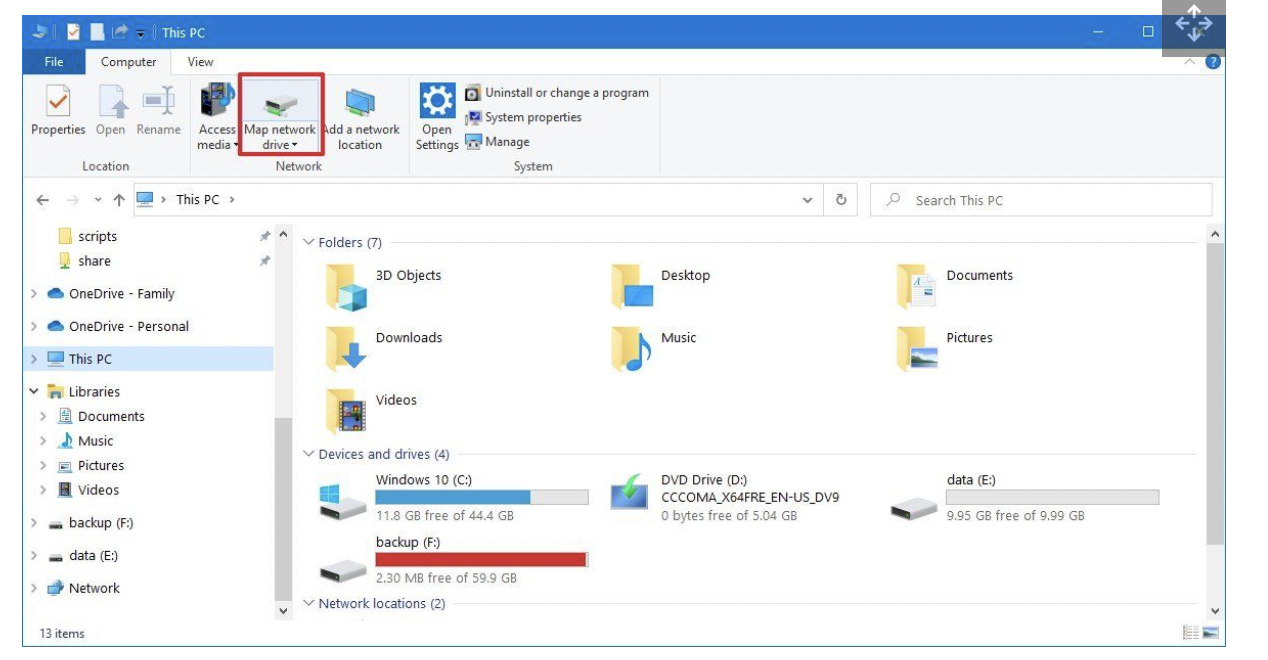
\includegraphics[width=0.8\linewidth]{images/nas_map10} \end{flushleft}

\begin{enumerate}
\def\labelenumi{\arabic{enumi}.}
\setcounter{enumi}{3}
\tightlist
\item
  Select a drive letter from the drop-down menu.

  \begin{enumerate}
  \def\labelenumii{\arabic{enumii}.}
  \setcounter{enumii}{4}
  \tightlist
  \item
    Enter \texttt{\textbackslash{}\textbackslash{}CCBNAS.dyn.ucr.edu\textbackslash{}pdo} into the folder field.
  \item
    Click Finish.
  \item
    Enter your Synology NAS username and password in the Windows credentials pop-up prompt.
  \end{enumerate}
\end{enumerate}

The mapped network drive will now appear within Windows Explorer as local storage, allowing you to quickly transfer files.

\begin{itemize}
\tightlist
\item
  For Macs:

  \begin{enumerate}
  \def\labelenumi{\arabic{enumi}.}
  \tightlist
  \item
    Open the Finder app.
  \item
    Click \texttt{Go} on top bar and select \texttt{Connect\ to\ Server}.
  \item
    Type in the CCB NAS IP: \texttt{smb://CCBNAS.dyn.ucr.edu/pdo}
  \item
    Enter \texttt{User\ Name} and \texttt{Passcode}.
  \end{enumerate}
\end{itemize}

There should be a connection set to the CCB NAS at the folder level.

\begin{flushleft}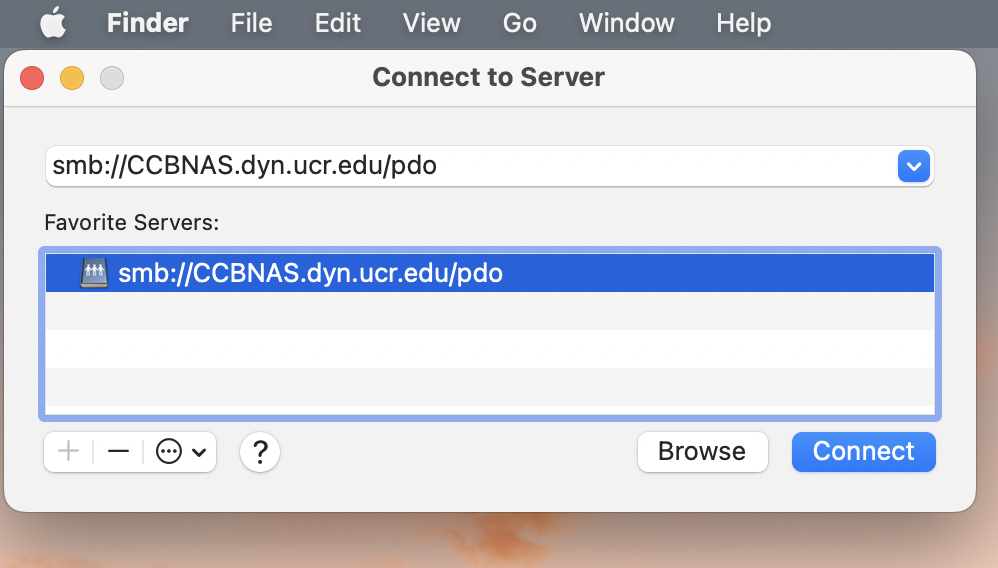
\includegraphics[width=0.5\linewidth]{images/nas_mac} \end{flushleft}

\hypertarget{connecting-the-ccb-nas-synology-to-git}{%
\subsection{Connecting the CCB NAS Synology to Git}\label{connecting-the-ccb-nas-synology-to-git}}

The information below was taken from the \href{https://kb.synology.com/en-sg/DSM/help/Git/git?version=7}{Synology Knowledge Center}.

Git is an open-source distributed version control system, which allows you to maintain software source code, documents, or any type of file on a computer with speed and efficiency.

\hypertarget{to-create-a-git-repository}{%
\subsubsection{To create a Git repository:}\label{to-create-a-git-repository}}

\begin{enumerate}
\def\labelenumi{\arabic{enumi}.}
\tightlist
\item
  Sign in to DSM using an account with administrative privileges.
\item
  Go to Control Panel \textgreater{} Terminal \& SNMP \textgreater{} Terminal then enable SSH service.
\item
  Go to Control Panel \textgreater{} Shared Folder and create a shared folder for Git repositories.
\item
  On your computer, enter the command below to access Synology NAS via SSH:
  \texttt{ssh\ {[}Synology\ NAS\ admin\ user\ name{]}@{[}Synology\ NAS\ IP\ address\ or\ hostname{]}\ -p\ {[}The\ port\ number\ of\ SSH{]}}
  For example, you can enter:
  \texttt{ssh\ myadminuser@192.168.1.2\ -p\ 22}
\item
  Enter the command below to change the current directory to the shared folder you created in step 3:
  \texttt{cd\ /{[}Volume\ name{]}/{[}Shared\ folder\ name{]}/}
  For example, you can enter:
  \texttt{cd\ /volume1/mysharefolder/}
\item
  Enter the command below to create a folder on your computer for the Git repository:
  \texttt{mkdir\ {[}Folder\ name{]}}
\item
  Enter the command below to change the current location to the new folder:
  \texttt{cd\ {[}Folder\ name{]}}
\item
  Enter the command below to create a Git bare repository under the folder you created in step 6:
  \texttt{git\ init\ -\/-bare}
\end{enumerate}

\begin{flushleft}
\includegraphics[width=0.85\linewidth]{images/git_root} \end{flushleft}

\hypertarget{to-allow-users-to-use-git-on-synology-nas-server}{%
\subsubsection{To Allow Users to Use Git on Synology NAS Server}\label{to-allow-users-to-use-git-on-synology-nas-server}}

\begin{enumerate}
\def\labelenumi{\arabic{enumi}.}
\tightlist
\item
  Sign in to DSM using an account with administrators' privileges.
\item
  Go to \textbf{Control Panel \textgreater{} Terminal \& SNMP \textgreater{} Terminal}, and enable \textbf{SSH service} for users to access Git repositories via SSH.
\item
  Go to \textbf{Control Panel \textgreater{} User \& Group} and create a user. Grant \textbf{Read/Write} permission of the Git repository shared folder to the user.
\item
  Go to \textbf{Package Center \textgreater{} Installed} and open the \textbf{Git Server} package.
\item
  Allow the user to access repositories via git-shell.
\end{enumerate}

\begin{flushleft}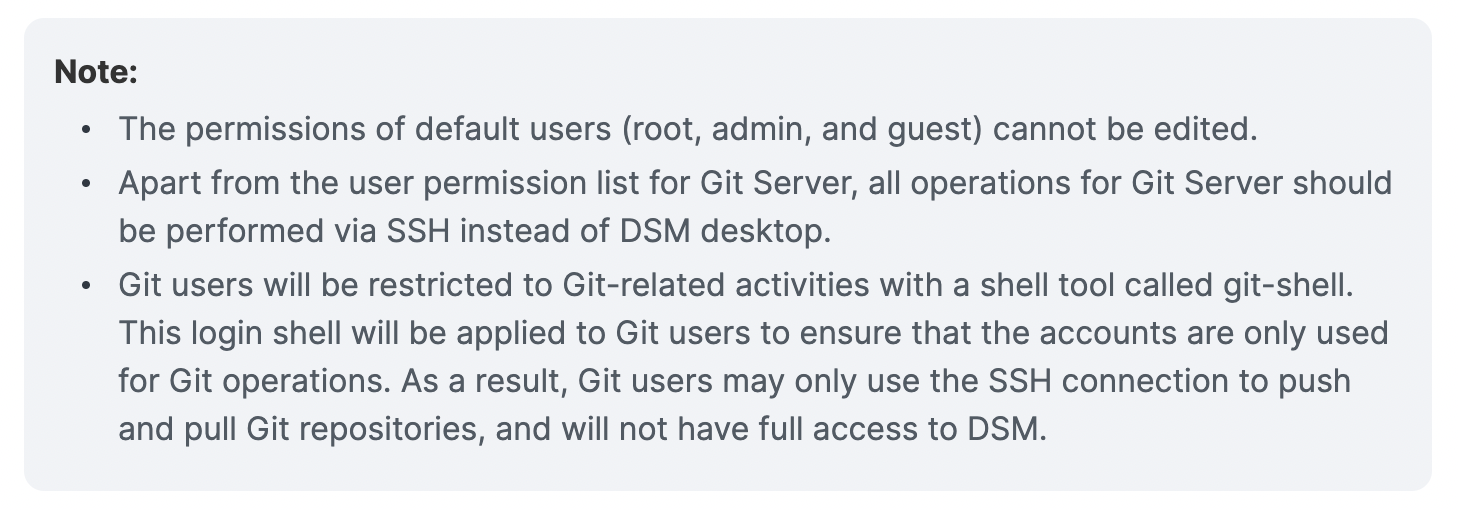
\includegraphics[width=0.85\linewidth]{images/git_usernote} \end{flushleft}

\hypertarget{google-apps}{%
\section{Google Apps}\label{google-apps}}

The CCB team utilizes a number of Google applications for project management, data \& file sharing, and communicating with colleagues.

\textbf{Google Calendar:} There is a lab Google calendar, \emph{UCR CCB Palm Desert}. This calendar maintains lab mates work and leave schedules as well as any team meetings. Please make sure this calendar is shared with you once you have obtained your UCR NetId.

\textbf{Google Drive:} CCB utilizes \emph{Shared Drive} folders as a file sharing application. You must request access to the shared drive folder from the lab P.I.

\textbf{Google Sites:} There is a \href{https://sites.google.com/ucr.edu/ccbucr/home}{CCB Google Site} that is in draft form at the moment. This site may serve as an intranet or provide public facing information in the future.

\hypertarget{microsoft-360-suite}{%
\section{Microsoft 360 Suite}\label{microsoft-360-suite}}

UCR provides free access to Microsoft Office 365 Pro Plus for faculty, staff, and students! Please note that the available applications differ between PC and Mac OS. To learn more about downloading Microsoft applications, please visit the
\href{https://ucrsupport.service-now.com/ucr_portal/?id=kb_article\&sys_id=0868da980f602f0086b7c7dce1050ee0}{UC Riverside Microsoft 360 information page}.

Microsoft 360 training resources can be found \href{https://support.microsoft.com/en-us/training}{here}.

\hypertarget{slack}{%
\section{Slack}\label{slack}}

\begin{flushleft}
\includegraphics[width=0.3\linewidth]{images/slack} \end{flushleft}

Slack is a messaging app that connects teams via channels and direct messages (DMs). To make the most of this team communication tool, you will need to download the application to your desktop, have the application open throughout the workday, and adjust the notification settings to your preferences to receive timely alerts.

\hypertarget{download-the-slack-app}{%
\subsection{Download the Slack app}\label{download-the-slack-app}}

\begin{itemize}
\tightlist
\item
  For Windows: download Slack \href{https://slack.com/downloads/windows}{here}.
\item
  For Macs: download Slack \href{https://slack.com/downloads/mac}{here}.
\item
  Consider adding the app to your Android or iOS device(s) for mobile communication with the CCB team!
\end{itemize}

\hypertarget{join-the-ccb_ucr-slack-workspace}{%
\subsection{Join the CCB\_UCR Slack Workspace}\label{join-the-ccb_ucr-slack-workspace}}

Follow \href{https://join.slack.com/t/ccbucr/shared_invite/zt-1dfpaguqs-F4CAPCI4ILMvT0JOcSpnag}{this link} to join the CCB Slack workspace. Once you have joined, you will be automatically be added to several workspace channels:

\begin{itemize}
\tightlist
\item
  \texttt{\#general}: a channel for general announcements and team-wide conversations
\item
  \texttt{\#how\_to\_slack}: a channel for tips for how to best use Slack and its apps, as well as a space for the team to ask questions re: how to best utilize this communication tool. Check out the \texttt{pinned} messages and \texttt{bookmarked} websites.
\item
  \texttt{\#meetings}: a channel for announcing meetings and sharing resources for team meetings.
\item
  \texttt{\#random}: a channel to share random news, updates, ideas, jokes, etc.
\end{itemize}

\hypertarget{slack-resources}{%
\subsection{Slack Resources}\label{slack-resources}}

The \href{https://slack.com/help/articles/360059928654-How-to-use-Slack--your-quick-start-guide}{Slack help center} has useful \emph{how to} guides and \href{https://slack.com/help/articles/360059976673-Slack-video-tutorials}{tutorials} to facilitate working in Slack.

\textbf{Slack Trainings}

Check out Slack's \href{https://slack.com/intl/en-in/resources/using-slack/top-5-tips-for-getting-started-in-slack}{\textbf{Top 5 tips for getting started in Slack}} (5 min read) to learn the app's basic functions and communication workflows.

The \href{https://slack.com/help/articles/360059928654-How-to-use-Slack--your-quick-start-guide}{Slack help center's ``how to'' guide} has several sections:

\begin{itemize}
\tightlist
\item
  \href{https://slack.com/help/articles/360059928654-How-to-use-Slack--your-quick-start-guide\#sidebar}{Quick Reference Guide} (20 min read)
\item
  \href{https://slack.com/help/categories/200111606}{Using Slack}: recommended Sections to review

  \begin{itemize}
  \tightlist
  \item
    Format \& style messages (5 min read)
  \item
    Message features \& tools (15 min read)
  \item
    Audio \& video (10 min read)
  \end{itemize}
\item
  \href{https://slack.com/help/categories/360000047906}{Your Profile}

  \begin{itemize}
  \tightlist
  \item
    Adjust your notifications: \href{https://slack.com/help/articles/201355156-Configure-your-Slack-notifications}{configure your notifications} (5 min read)
  \item
    Change your settings \& preferences:

    \begin{itemize}
    \tightlist
    \item
      \href{https://slack.com/help/articles/201864558-Set-your-Slack-status-and-availability}{set your Slack status \& availability} (3 min read)
    \item
      \href{https://slack.com/help/articles/212596808-Adjust-your-sidebar-preferences}{adjust your sidebar preferences} (3 min read)
    \end{itemize}
  \end{itemize}
\item
  Connect Tools

  \begin{itemize}
  \tightlist
  \item
    Connect tools from the Slack app directory: \href{https://slack.com/help/articles/202035138-Add-apps-to-your-Slack-workspace}{add apps to your Slack workspace} (3 min read)
  \end{itemize}
\item
  \href{https://slack.com/help/categories/360000049063}{Tutorials} - a long list of tutorials to review as needed and as time allows
\end{itemize}

\textbf{Slack Apps}

Up to 10 Slack apps are available for free Slack accounts, and unlimited apps are available for Pro Slack accounts.

\begin{itemize}
\tightlist
\item
  A \textbf{Trello app} is incorporated in the CCB\_UCR Slack workspace. You can create cards in Slack for the CCB Team Projects Trello workspace. To learn how, \href{https://slack.com/help/articles/231967387-Trello-for-Slack}{follow this Slack connect tool}.
\item
  The \textbf{Zoom app} can be added to Slack that allows your to start or join a Zoom Meeting or Zoom Phone call by using the \textbf{``/zoom''} slash command in any Slack channel or message.
\item
  Add the \textbf{Google Drive app} to Slack to share resources from the CCB Shared Drive.
\item
  There is an app for \textbf{Microsoft Teams} which allows a Teams video call from Slack.

  \begin{itemize}
  \tightlist
  \item
    Start a Teams video call right from Slack
    Launch a call in Slack with the /teams-calls slash command. Before joining, get a quick glance at who's already on the call and when the call kicked off.
  \item
    Jump from Slack straight into a meeting --- join Teams meetings directly from calendar reminders in Slack, using the Outlook or Google Calendar apps.
  \item
    Customize call settings for your team. Set Microsoft Teams Calls as your default calling provider, so anyone can start a video call in Teams with a quick click of the phone button in Slack.
  \end{itemize}
\end{itemize}

\textbf{Other cool Slack workspaces to join:}

\begin{itemize}
\item
  \href{https://eco-data-science.github.io/}{EcoDataScience} - an environmental data science study group that started at UC Santa Barbara, but now has an international following!
\item
  \href{https://www.rfordatasci.com}{R4DS Online Learning Community}
\item
  \href{https://www.sortee.org}{Society for Open, Reliable, and Transparent Ecology and Evolutionary Biology (SORTEE)}
\end{itemize}

\hypertarget{trello}{%
\section{Trello}\label{trello}}

\begin{flushleft}
\includegraphics[width=0.3\linewidth]{images/trello} \end{flushleft}

\href{https://trello.com/en}{Trello} is a project management app tool that provides teams the opportunity to create task lists, reference \& resource lists, and communicate via tagging! To connect with CCB's Trello Workspace, send a request to CCB's PI. The main board is \textbf{CCB Team Projects}.

\hypertarget{zoom}{%
\section{Zoom}\label{zoom}}

Zoom is a great tool to schedule virtual meetings, and the CCB hosts Zoom-based team meeting regularly. UC Riverside provides all faculty, staff, and students a free premium account. In order to utilize this service, download the application and sign in via Single Sign-ON (SS0). For the most current installation and log in information, visit UC Riverside's \href{https://its.ucr.edu/blog/2019/12/17/changes-ucr-zoom-account-access}{Information Technology Systems Zoom account page}.

\begin{itemize}
\tightlist
\item
  \textbf{Step 1}: Download the Zoom application via \href{https://ucr.zoom.us/}{UC Riverside's Zoom service page} - just select the \textbf{Download} button!
\end{itemize}

\begin{center}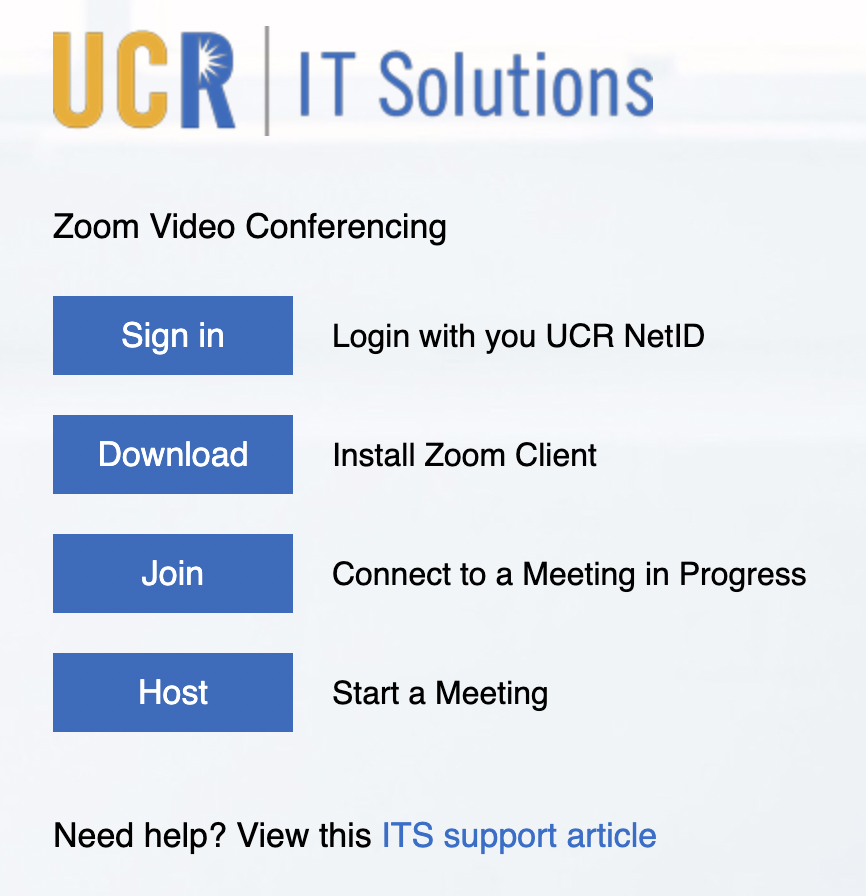
\includegraphics[width=0.75\linewidth]{images/zoomdownload} \end{center}

\begin{itemize}
\item
  \textbf{Step 2}: Once the application is downloading, Zoom will automatically open. You will be prompted to either \emph{Join a Meeting} or \emph{Sign In}. Select \emph{Sign In} and set up your UCR Zoom account using your NetId information.
\item
  \textbf{Step 3}: Click the \emph{Sign In with SSO} button, then enter \texttt{ucr} in the \emph{company domain} section.
\end{itemize}

\begin{center}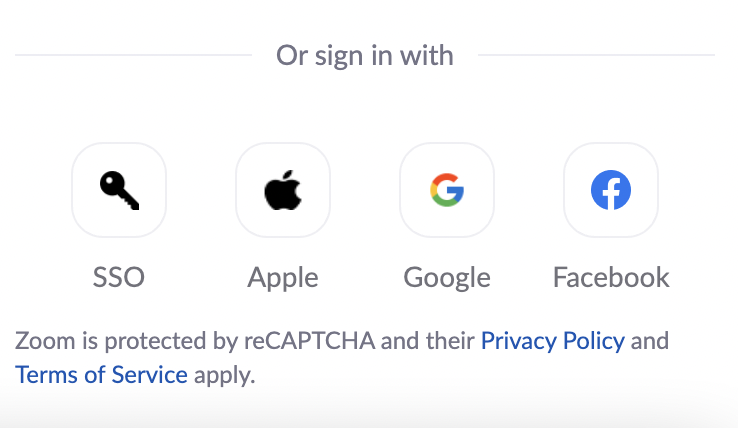
\includegraphics[width=0.6\linewidth]{images/zoomsso} \end{center}

\begin{center}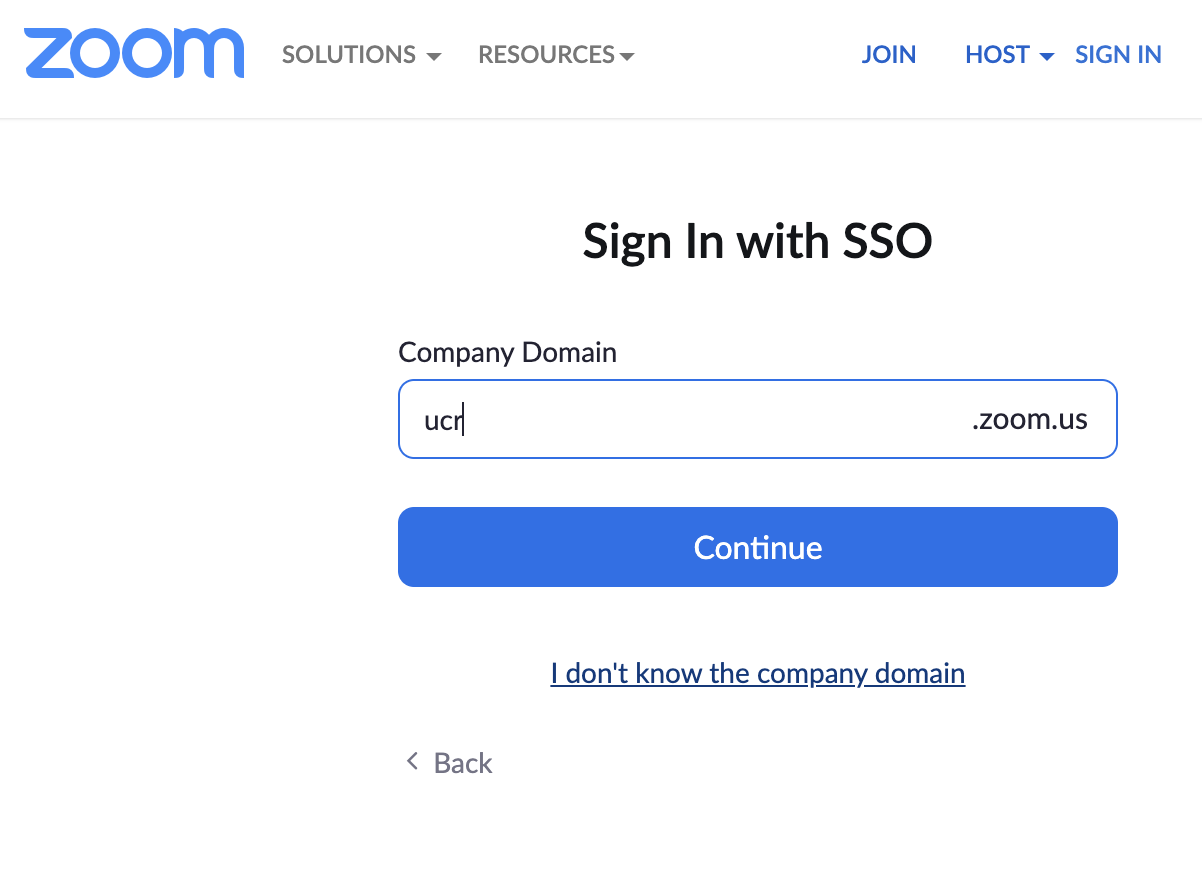
\includegraphics[width=0.75\linewidth]{images/zoomdomain} \end{center}

\begin{itemize}
\tightlist
\item
  \textbf{Step 4}: You will then be prompted to sign in, this time using your UCR NetId. The program may open up an authentication window requesting your UCR NetId as shown below:
\end{itemize}

\begin{center}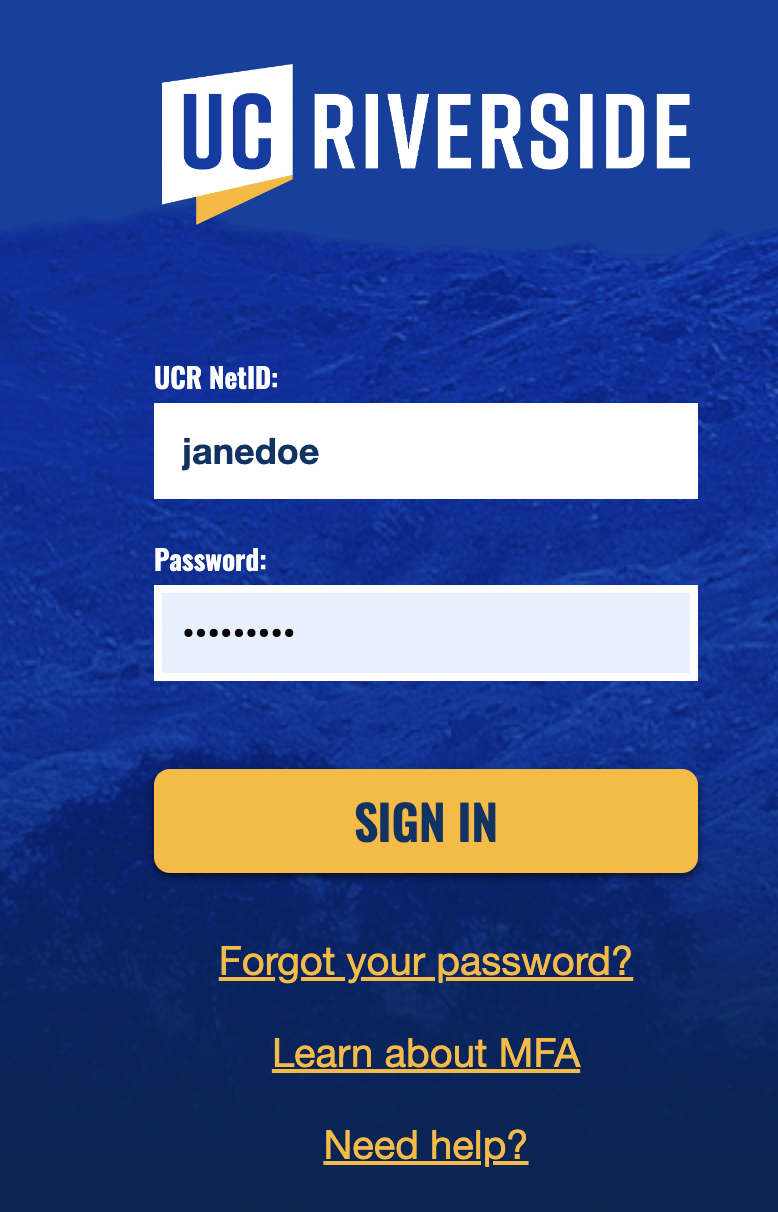
\includegraphics[width=0.6\linewidth]{images/zoomcred} \end{center}

\begin{itemize}
\tightlist
\item
  \textbf{Step 5}: Personalize your Zoom account! You can add your name, pronouns, and an image to your profile, create a \emph{personal Zoom room} to utilize as a default meeting space, and set settings like \emph{mute all participants when they join a meeting} or turn off settings such as \emph{start meetings with participant video on. Participants can change this during the meeting.}
\end{itemize}

Happy Zooming!

\textbf{Zoom Resources:}

\begin{itemize}
\tightlist
\item
  \href{https://support.zoom.us/hc/en-us}{Zoom Help Desk}
\item
  \href{https://livetraining.zoom.us/rec/play/6Zx8f-j7qDw3GNeQswSDAPJ-W9S4J6qshiYfqfcNyk20WyIHNFChb7pHZuClKrDVR76R1BxgtMF4txaS?continueMode=true}{Zoom meetings trainings}
\item
  \href{https://ucr.zoom.us/}{UC Riverside Zoom Services}
\end{itemize}

\hypertarget{zotero}{%
\section{Zotero}\label{zotero}}

The Center for Conservation Biology shares research references through Zotero software. Zotero is a citation management tool and allows groups to collect and share references easily. The Zotero browser extension makes it easy to copy citations from webpages.

To install Zotero and the extension, please follow UC Riverside's installation instructions \href{https://guides.lib.ucr.edu/c.php?g=171064}{here}. \emph{Note}: These instructions are for a \textbf{Windows} machine, but it is a similar process for Macs.

\begin{center}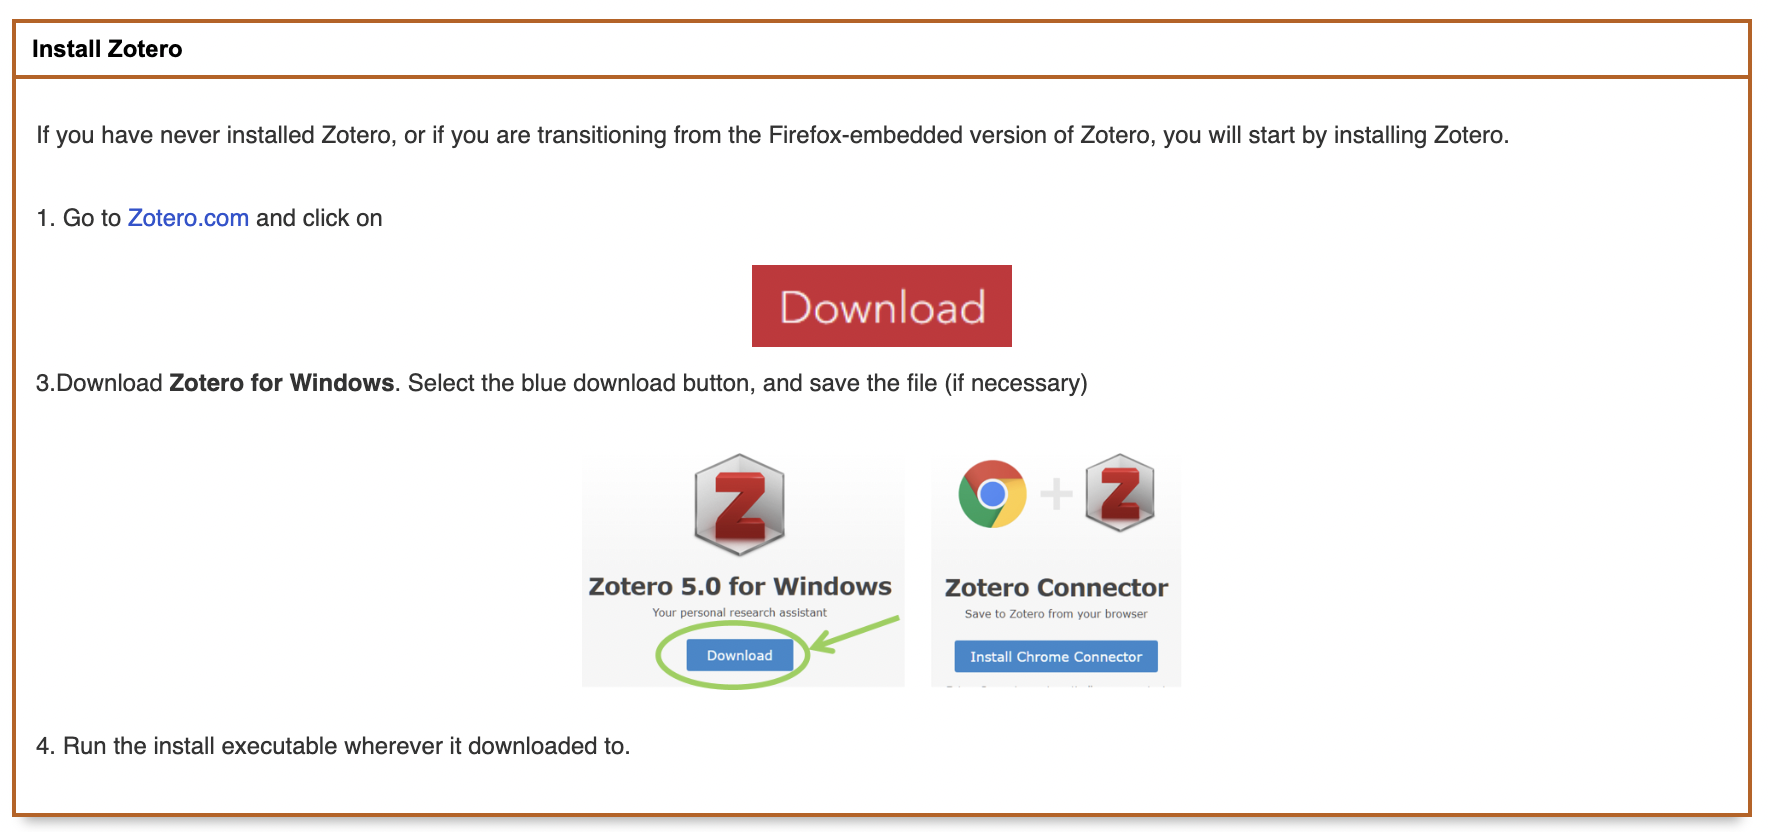
\includegraphics[width=0.8\linewidth]{images/zoteroinstall} \end{center}

\begin{center}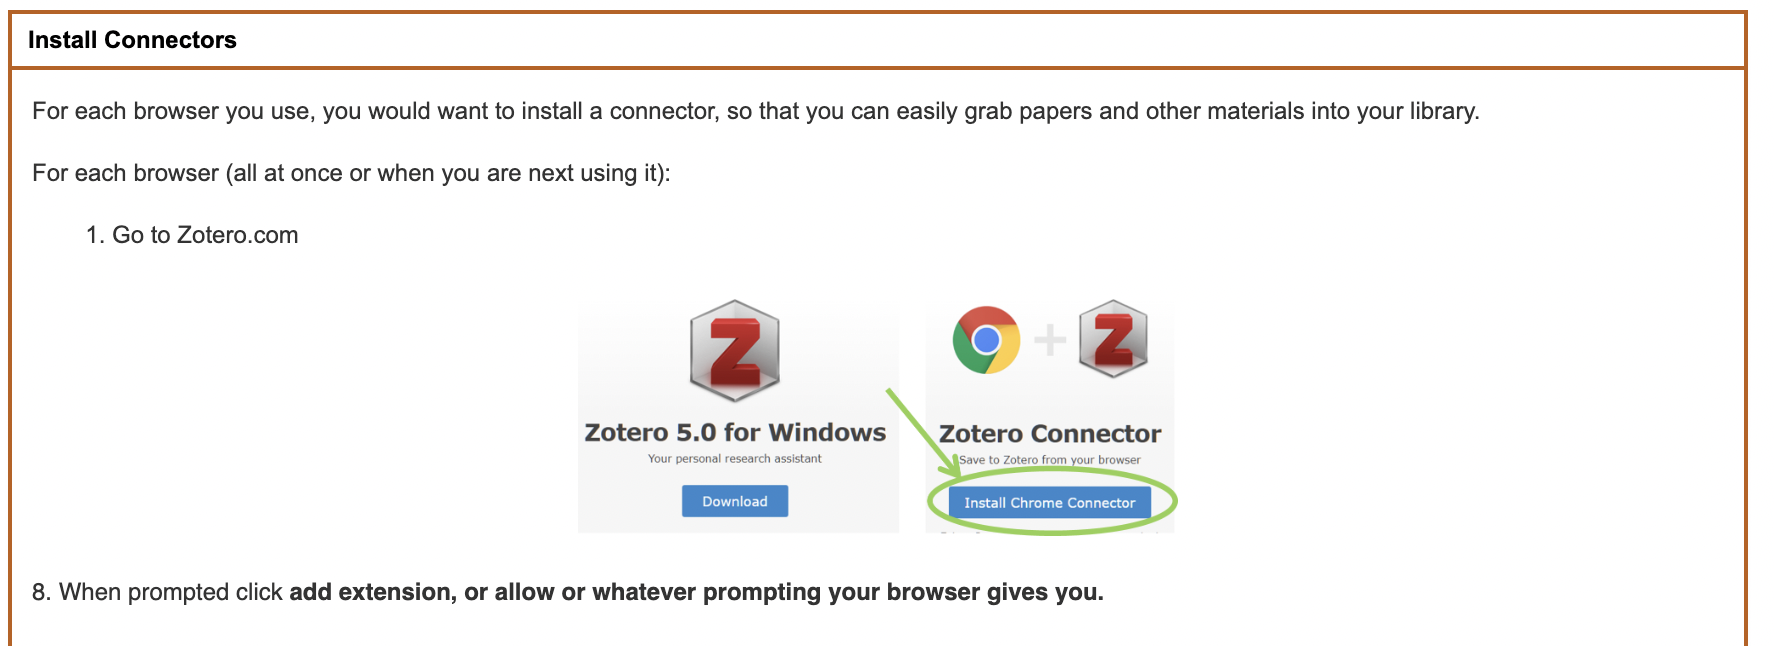
\includegraphics[width=0.8\linewidth]{images/zoteroextension} \end{center}

The next step is to create a Zotero account and enable syncing to enable extension use and to be able to join the \href{https://www.zotero.org/groups/4734848/ccbucr}{CCB Zotero Reference Group}. Make sure to use your using the UCR email address when setting up the Zotero account.

\begin{center}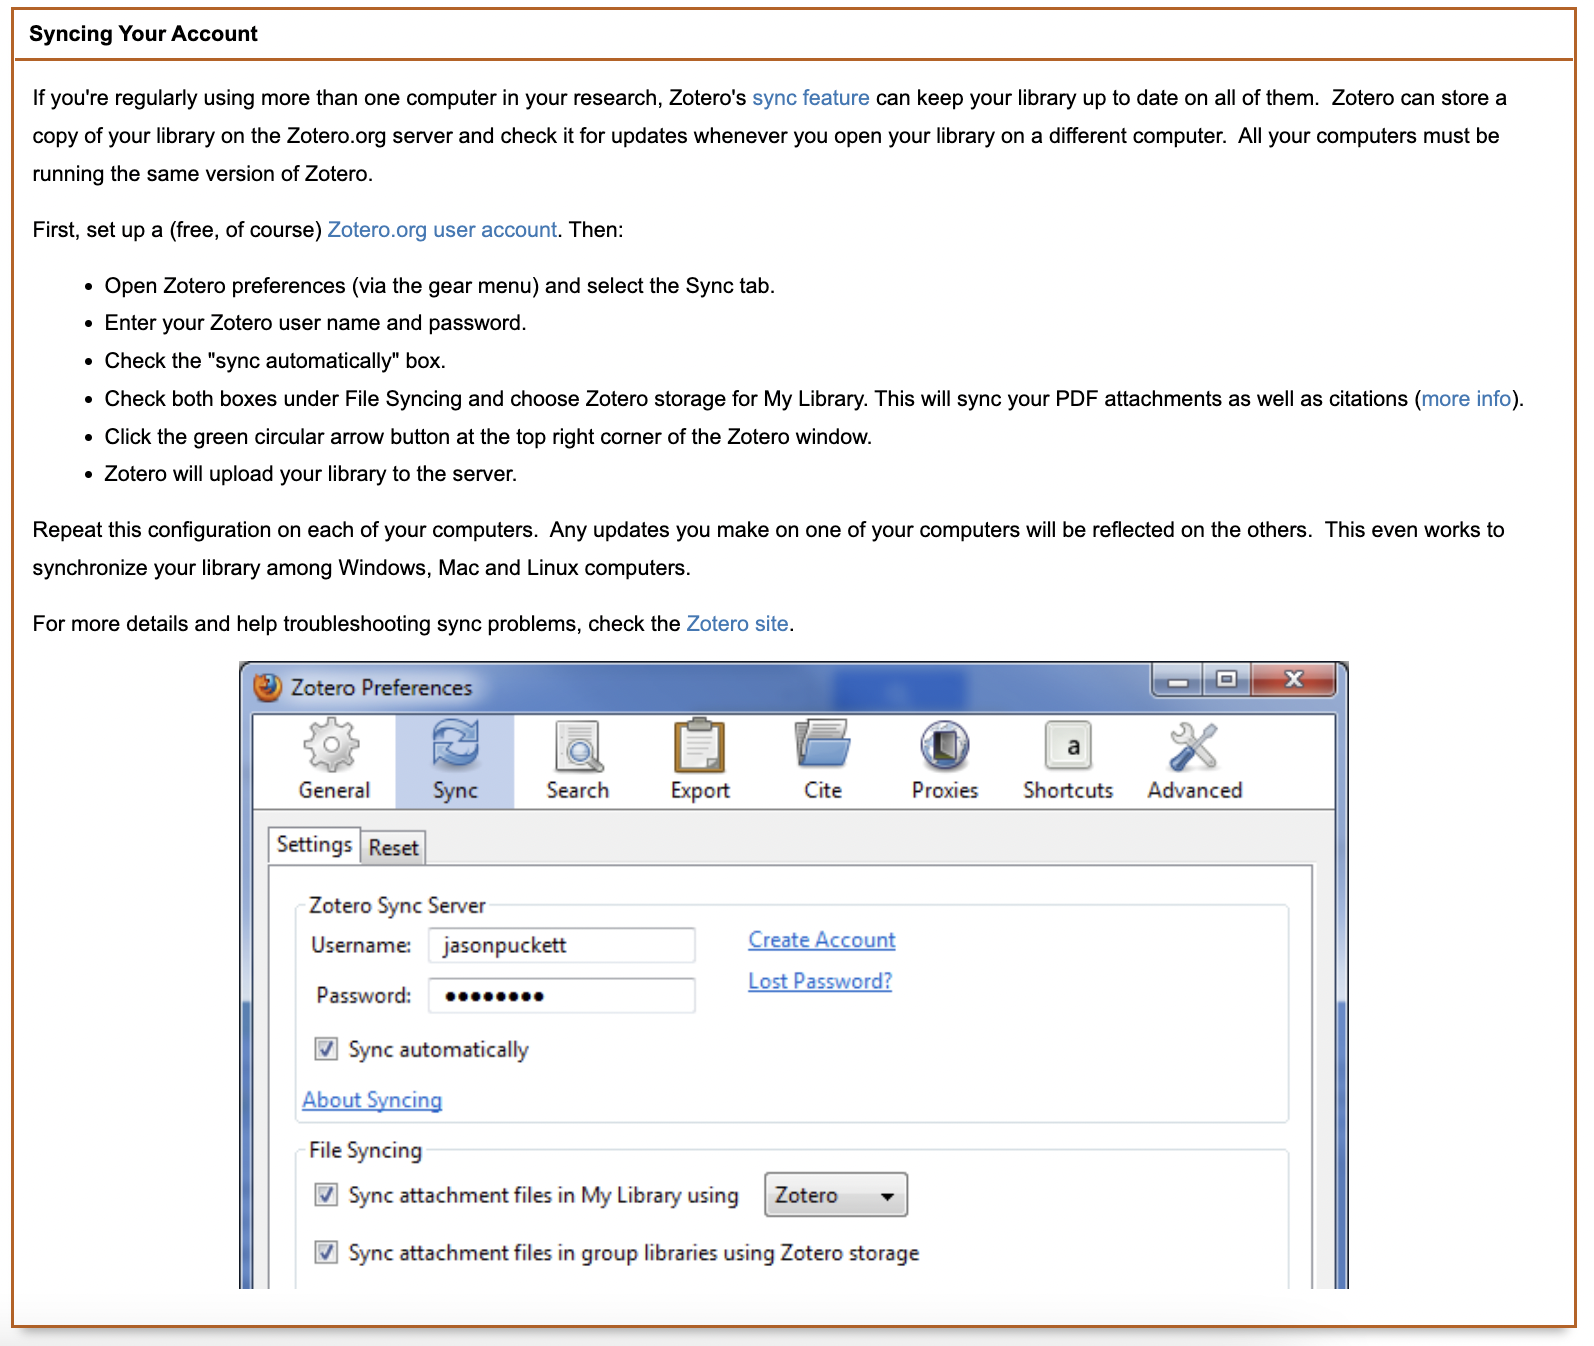
\includegraphics[width=0.8\linewidth]{images/zoterosyncing} \end{center}

To connect to the CCB Zotero Reference Group, navigate to \href{https://www.zotero.org/groups/4734848/ccbucr}{this link}. If you do not have access to the Group page, please send a request that you be added to the CCB PI.

For more information on how to use Zotero, check out these links:

\begin{itemize}
\tightlist
\item
  \href{https://guides.lib.ucr.edu/c.php?g=171064\&p=1126842}{UC Riverside Zotero Tips \& Tricks}
\item
  \href{https://www.zotero.org/support/quick_start_guide}{Zotero Quick Start Guide}
\item
  \href{https://www.zotero.org/support/groups}{Zotero Groups}
\item
  \href{https://www.youtube.com/watch?v=zuuOYjE8m98}{RStudio Citations} - add BibTex citation format in Zotero then quickly use .bib files in R to create references in markdown.
\end{itemize}

\hypertarget{esri}{%
\chapter{ESRI GIS Platform}\label{esri}}

\hypertarget{esri-arcgis}{%
\section{ESRI ArcGIS}\label{esri-arcgis}}

UC Riverside provides free access to ESRI ArcGIS software and platforms for faculty, staff, and students. Learn more about these data analysis and visualization tools \href{https://ucrsupport.service-now.com/ucr_portal?id=sc_category\&sys_id=e9b36a7e1b691c10eab58734ec4bcb78\&catalog_id=-1}{here}.

\textbf{ESRI Platform Software}

\begin{itemize}
\tightlist
\item
  \textbf{ESRI ArcGIS Desktop}: a proprietary desktop GIS software suite that allows you to create maps, perform spatial analysis and manage data. Required software for installation: Microsoft .NET (aka a PC machine), Python 2.7+.
\item
  \textbf{ESRI ArcGIS Pro}: ArcGIS Desktop is transitioning to ArcGIS Pro, an interactive spatial data visualization tool that allows users to create 2D maps, 3D scenes, and share projects on ArcGIS Online. Training resources for ArcGIS Pro are \href{https://www.esri.com/en-us/arcgis/products/arcgis-pro/resources}{here}.
\item
  \textbf{ESRI ArcGIS Online}: This is cloud-based software that runs on any device with an internet connection. It allows users to easily publish maps on-line, access other UCR spatial products, and create spatial data dashboards and hubs. Check out \href{https://ucr.maps.arcgis.com/home/index.html}{UCR ArcGIS Online}.
\end{itemize}

\hypertarget{install-esri-arcgis-software}{%
\section{Install ESRI ArcGIS software}\label{install-esri-arcgis-software}}

For additional installation information, navigate to \href{https://ucrsupport.service-now.com/ucr_portal?id=kb_article\&sys_id=0231b6e21b095190453e7592cd4bcbaf}{UCR's ServiceLink Access ArcGIS Online and ArcGIS Pro help page}.

\hypertarget{esri-arcgis-online}{%
\subsection{ESRI ArcGIS Online}\label{esri-arcgis-online}}

Instructions for how to sign in to ArcGIS Online via UCR.

\begin{itemize}
\item
  \textbf{Step 1:} Navigate to the \href{https://ucr.maps.arcgis.com/home/index.html}{UCR's Academic ArcGIS Online site}.
\item
  \textbf{Step 2:} Click on the `Sign In' link at the top right hand corner of the landing page.
\end{itemize}

\begin{center}
\includegraphics[width=0.75\linewidth]{images/esri_arcgisonline} \end{center}

\begin{itemize}
\tightlist
\item
  \textbf{Step 3:} Select the \textbf{UCR University of California, Riverside Enterprise login} (blue button) option.
\end{itemize}

\begin{center}
\includegraphics[width=0.6\linewidth]{images/esri_ucrenterprise} \end{center}

\begin{itemize}
\tightlist
\item
  \textbf{Step 4:} Sign in with UCR Net ID and Password
\end{itemize}

\begin{center}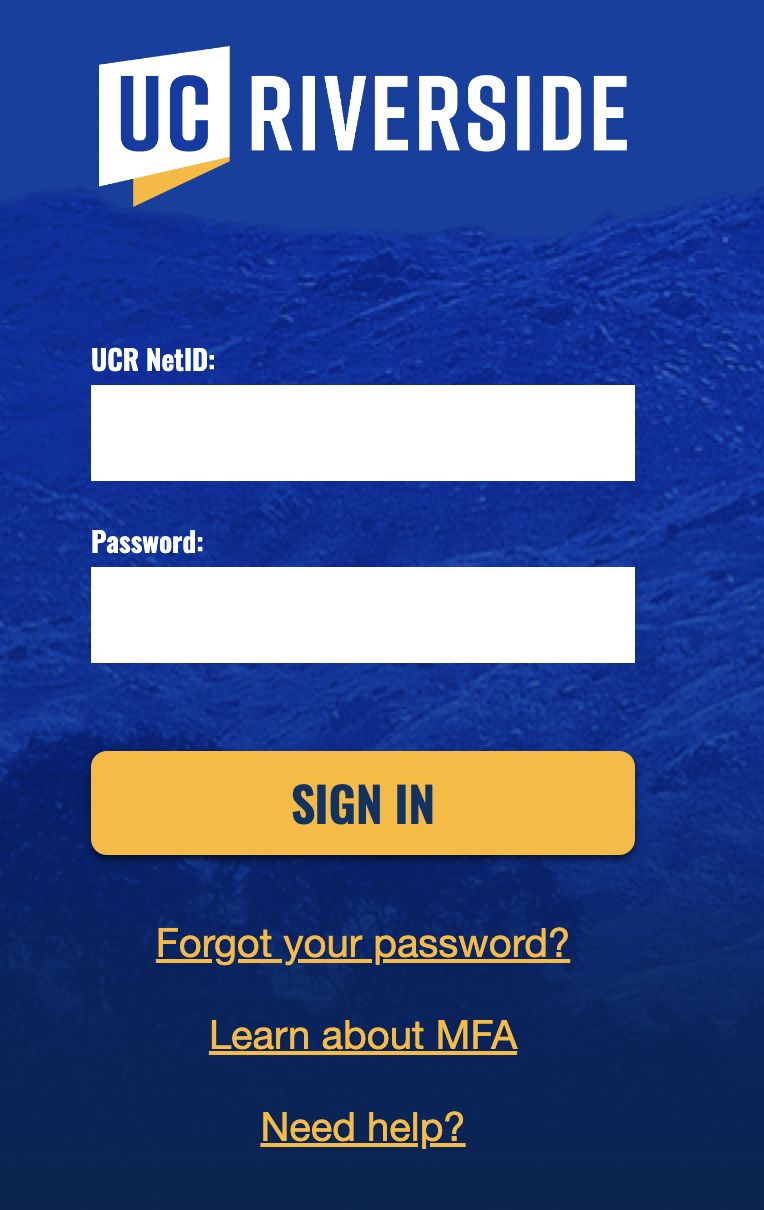
\includegraphics[width=0.55\linewidth]{images/esri_ucrid} \end{center}

\hypertarget{esri-arcgis-pro}{%
\subsection{ESRI ArcGIS Pro}\label{esri-arcgis-pro}}

Instructions for how to download ArcGIS Pro from UCR's ArcGIS Online.

\begin{itemize}
\item
  \textbf{Step 1:} Navigate to the UCR's Academic Instance of \href{https://ucr.maps.arcgis.com/home/index.html}{ArcGIS Online}.
\item
  \textbf{Step 2:} Click on the \texttt{Sign\ In} link at the top right hand corner of the landing page.
\end{itemize}

\begin{center}
\includegraphics[width=0.75\linewidth]{images/esri_signin} \end{center}

\begin{itemize}
\item
  \textbf{Step 3:} Select the \textbf{UCR University of California, Riverside Enterprise login} (blue button) option under UCR.
\item
  \textbf{Step 4:} At the top right of the page, click your user name and click \texttt{My\ Settings}.
\item
  \textbf{Step 5:} On the \texttt{My\ Settings} page, click the Licenses tab.
\item
  \textbf{Step 6:} Scroll down, next to ArcGIS Pro, click \texttt{Download\ ArcGIS\ Pro}.
\end{itemize}

\begin{center}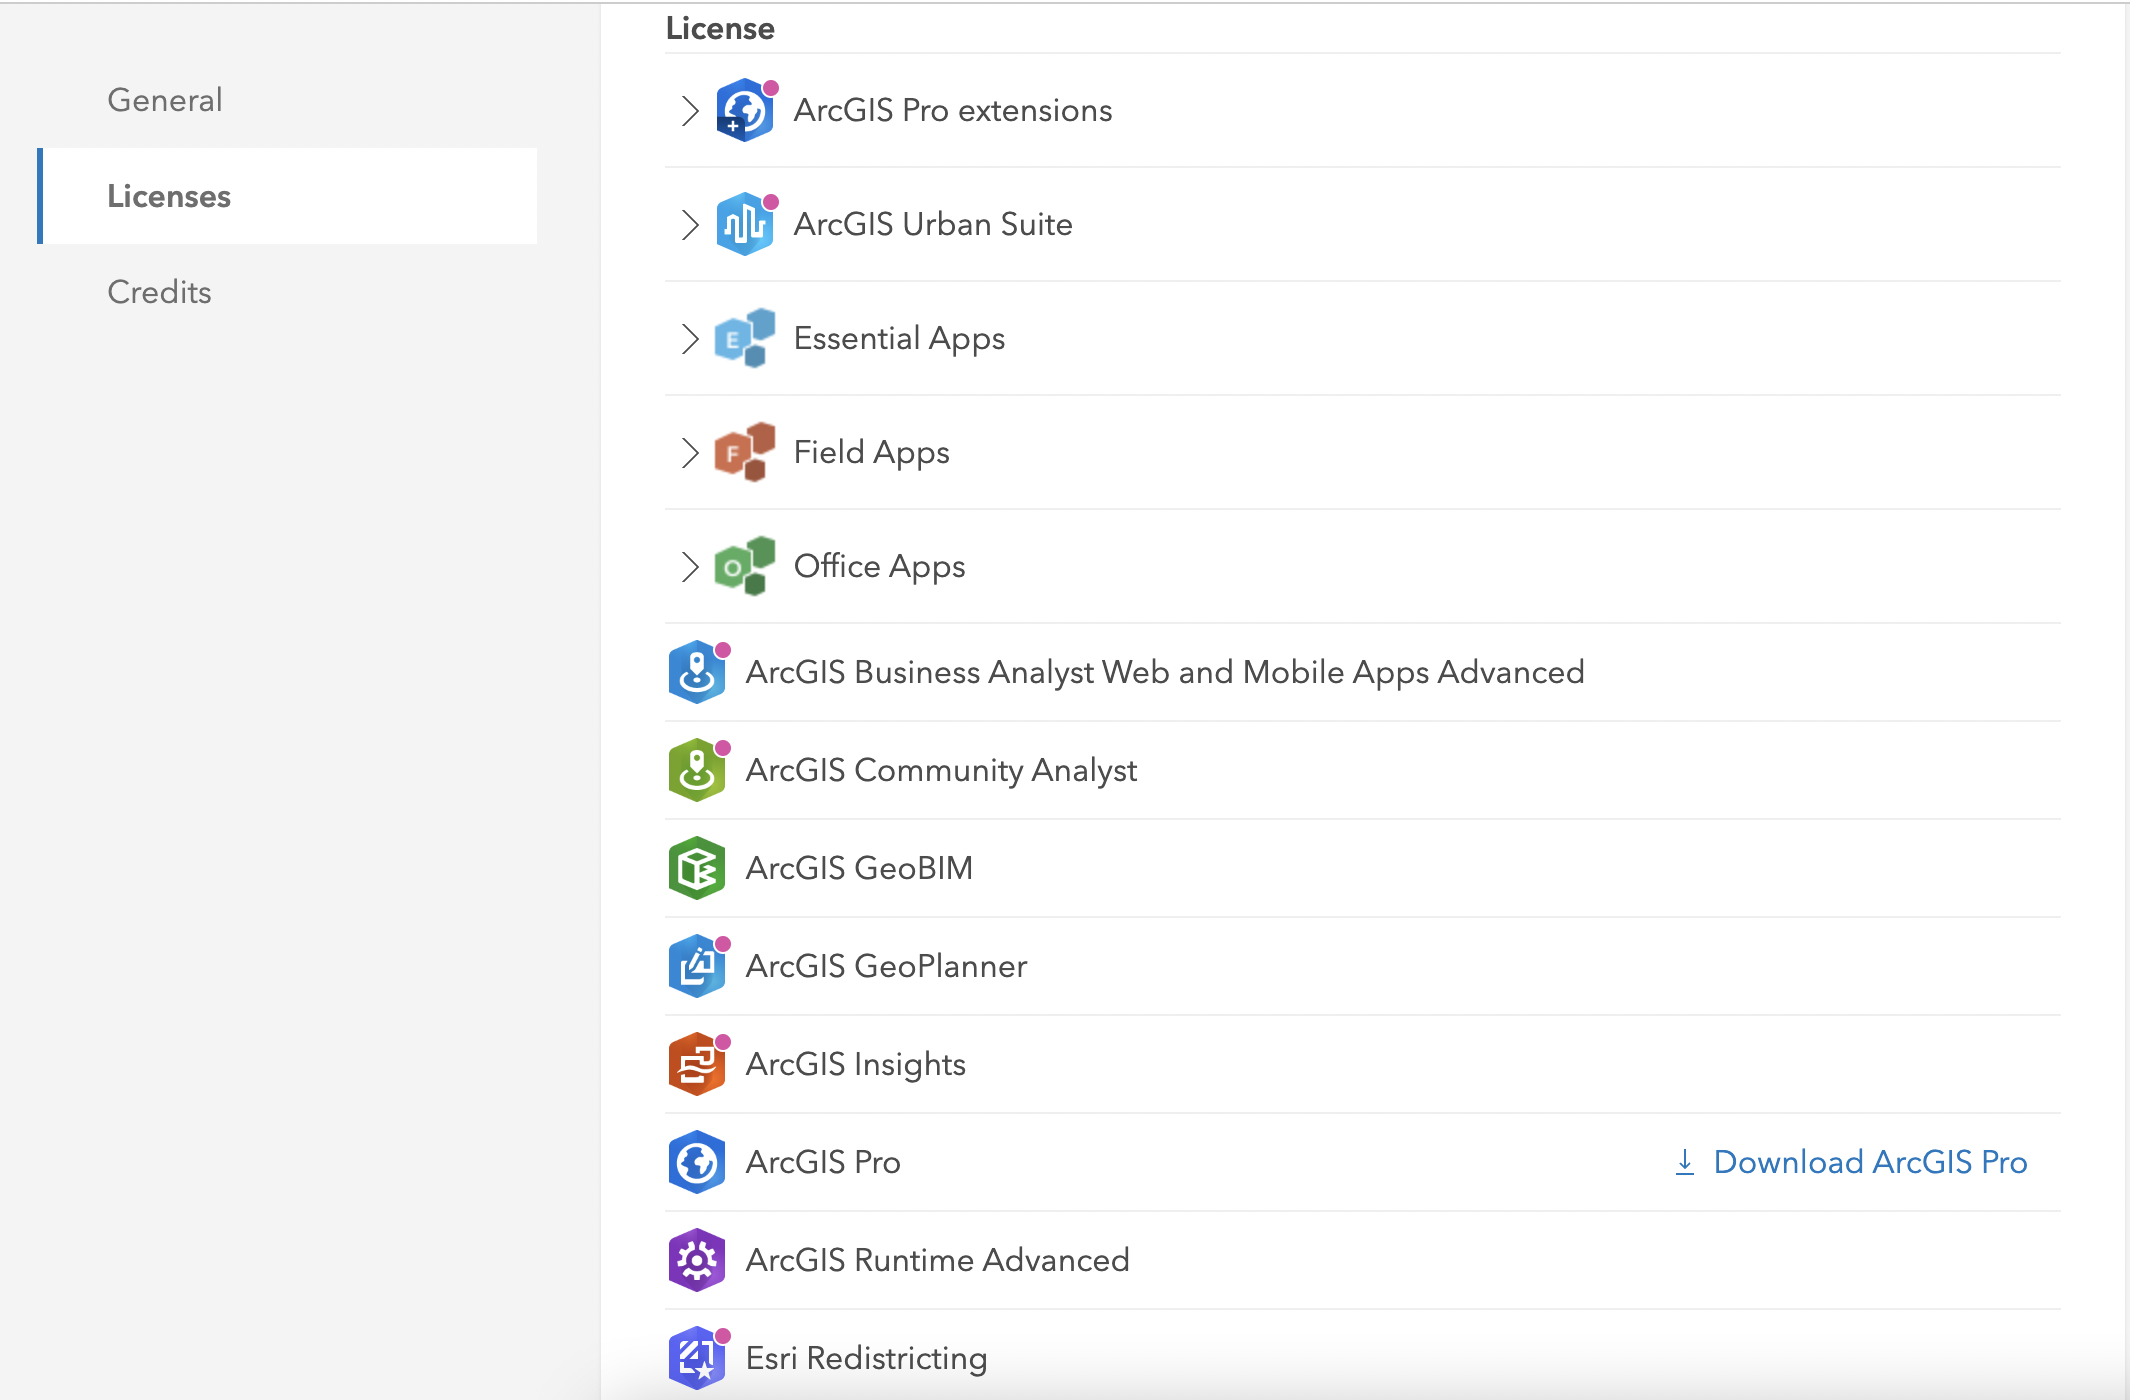
\includegraphics[width=0.75\linewidth]{images/esri_pro} \end{center}

\hypertarget{archived-ucr-esri-arcgis-desktop-and-pro-installation-instructions}{%
\subsubsection{Archived UCR ESRI ArcGIS Desktop and Pro Installation Instructions}\label{archived-ucr-esri-arcgis-desktop-and-pro-installation-instructions}}

This was the installation process prior to 2020. If there are issues with the above instructions, this is an alternative method to access ESRI software.

\begin{itemize}
\item
  \textbf{Step 1:} Navigate to the \href{https://ucrsupport.service-now.com/ucr_portal}{UCR Portal ServiceLink Software Catalog}.
\item
  \textbf{Step 2:} Under the Information Technology section, select \textbf{Request Services \& Software} link.
\end{itemize}

\begin{center}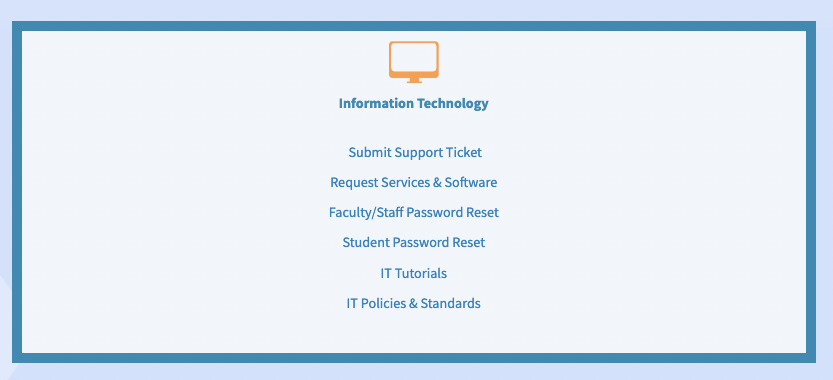
\includegraphics[width=0.75\linewidth]{images/ServiceLink} \end{center}

\begin{itemize}
\tightlist
\item
  \textbf{Step 3:} Scroll down to the \textbf{Software Request} card and select link.
\end{itemize}

\begin{center}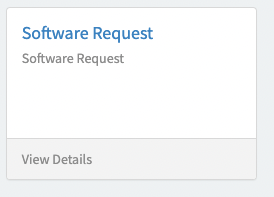
\includegraphics[width=0.45\linewidth]{images/softwarerequest} \end{center}

\begin{itemize}
\tightlist
\item
  \textbf{Step 4:} Complete the Software Request form using your UCR NetId and UCR email, then select \textbf{Submit}.
\end{itemize}

\begin{center}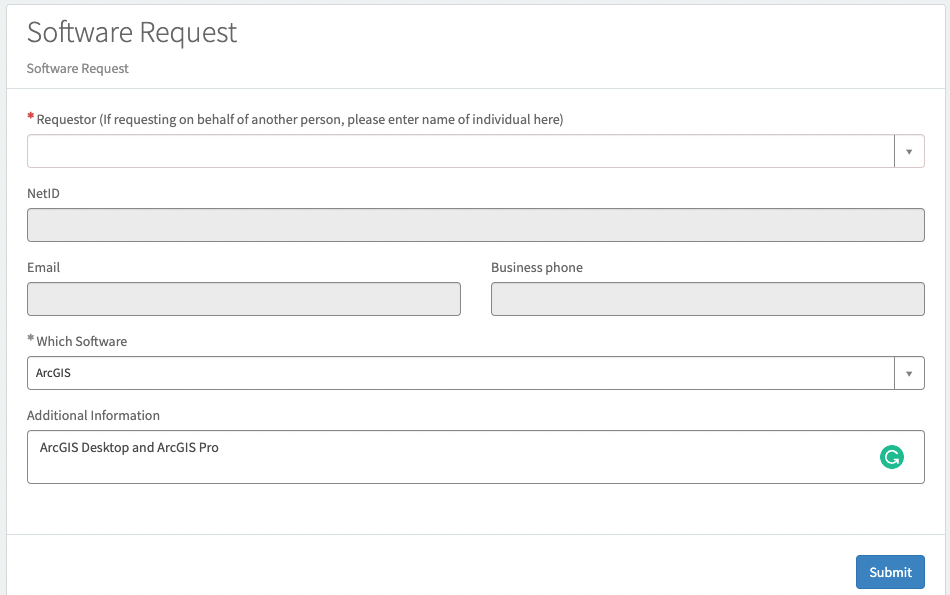
\includegraphics[width=0.75\linewidth]{images/requestsubmit} \end{center}

\begin{itemize}
\tightlist
\item
  \textbf{Step 5:} The UC IT team will send email notifications to provide further instructions.
\end{itemize}

\hypertarget{esri-resources}{%
\subsection{ESRI Resources}\label{esri-resources}}

Here are few resources that provide tutorials and workshops on how to use ESRI software:

\begin{itemize}
\tightlist
\item
  \textbf{ESRI Academy}: Search the ESRI Acadmey \href{https://www.esri.com/training/}{Course Catalog} for MOOCs, Tutorials, and Web Courses.
\item
  \textbf{UC ANR IGIS} - the \href{https://igis.ucanr.edu/Training/}{UC Agriculture and Natural Resources Informatics \& GIS Program} host ESRI ArcGIS training webinars and virtual workshops throughout the year.
\item
  \textbf{LinkedIn Learning} - Through \href{https://www.linkedin.com/learning/topics/arcgis?u=26135898}{UCR LinkedIn Learning}, users may take ESRI ArcGIS courses and learning paths.
\end{itemize}

\hypertarget{organization}{%
\chapter{Directory Organization \& Data Project Development}\label{organization}}

\hypertarget{file-naming}{%
\section{File Naming}\label{file-naming}}

When creating file names, best practices dictate that you should:

\begin{itemize}
\tightlist
\item
  Create meaningful but brief names. Limit a file name to 25 characters, if possible;
\item
  Use file names to classify types of files

  \begin{itemize}
  \tightlist
  \item
    ex: \texttt{20230131\_DTLA\_RA.csv} file name classifies this file as Rapid Assessment vegetation monitoring data from the Desert Tortoise Linkage Area and was created on Jan.~31, 2023;
  \end{itemize}
\item
  Avoid using spaces, dots and special characters (ex: \& or ? or !);
\item
  Use capital letters to delimit words (aka UpperCamelCase), not spaces or underscores for \textbf{data files}.(ex: \texttt{20170217CVStormwaterVAP.csv});
\end{itemize}

\begin{figure}

{\centering 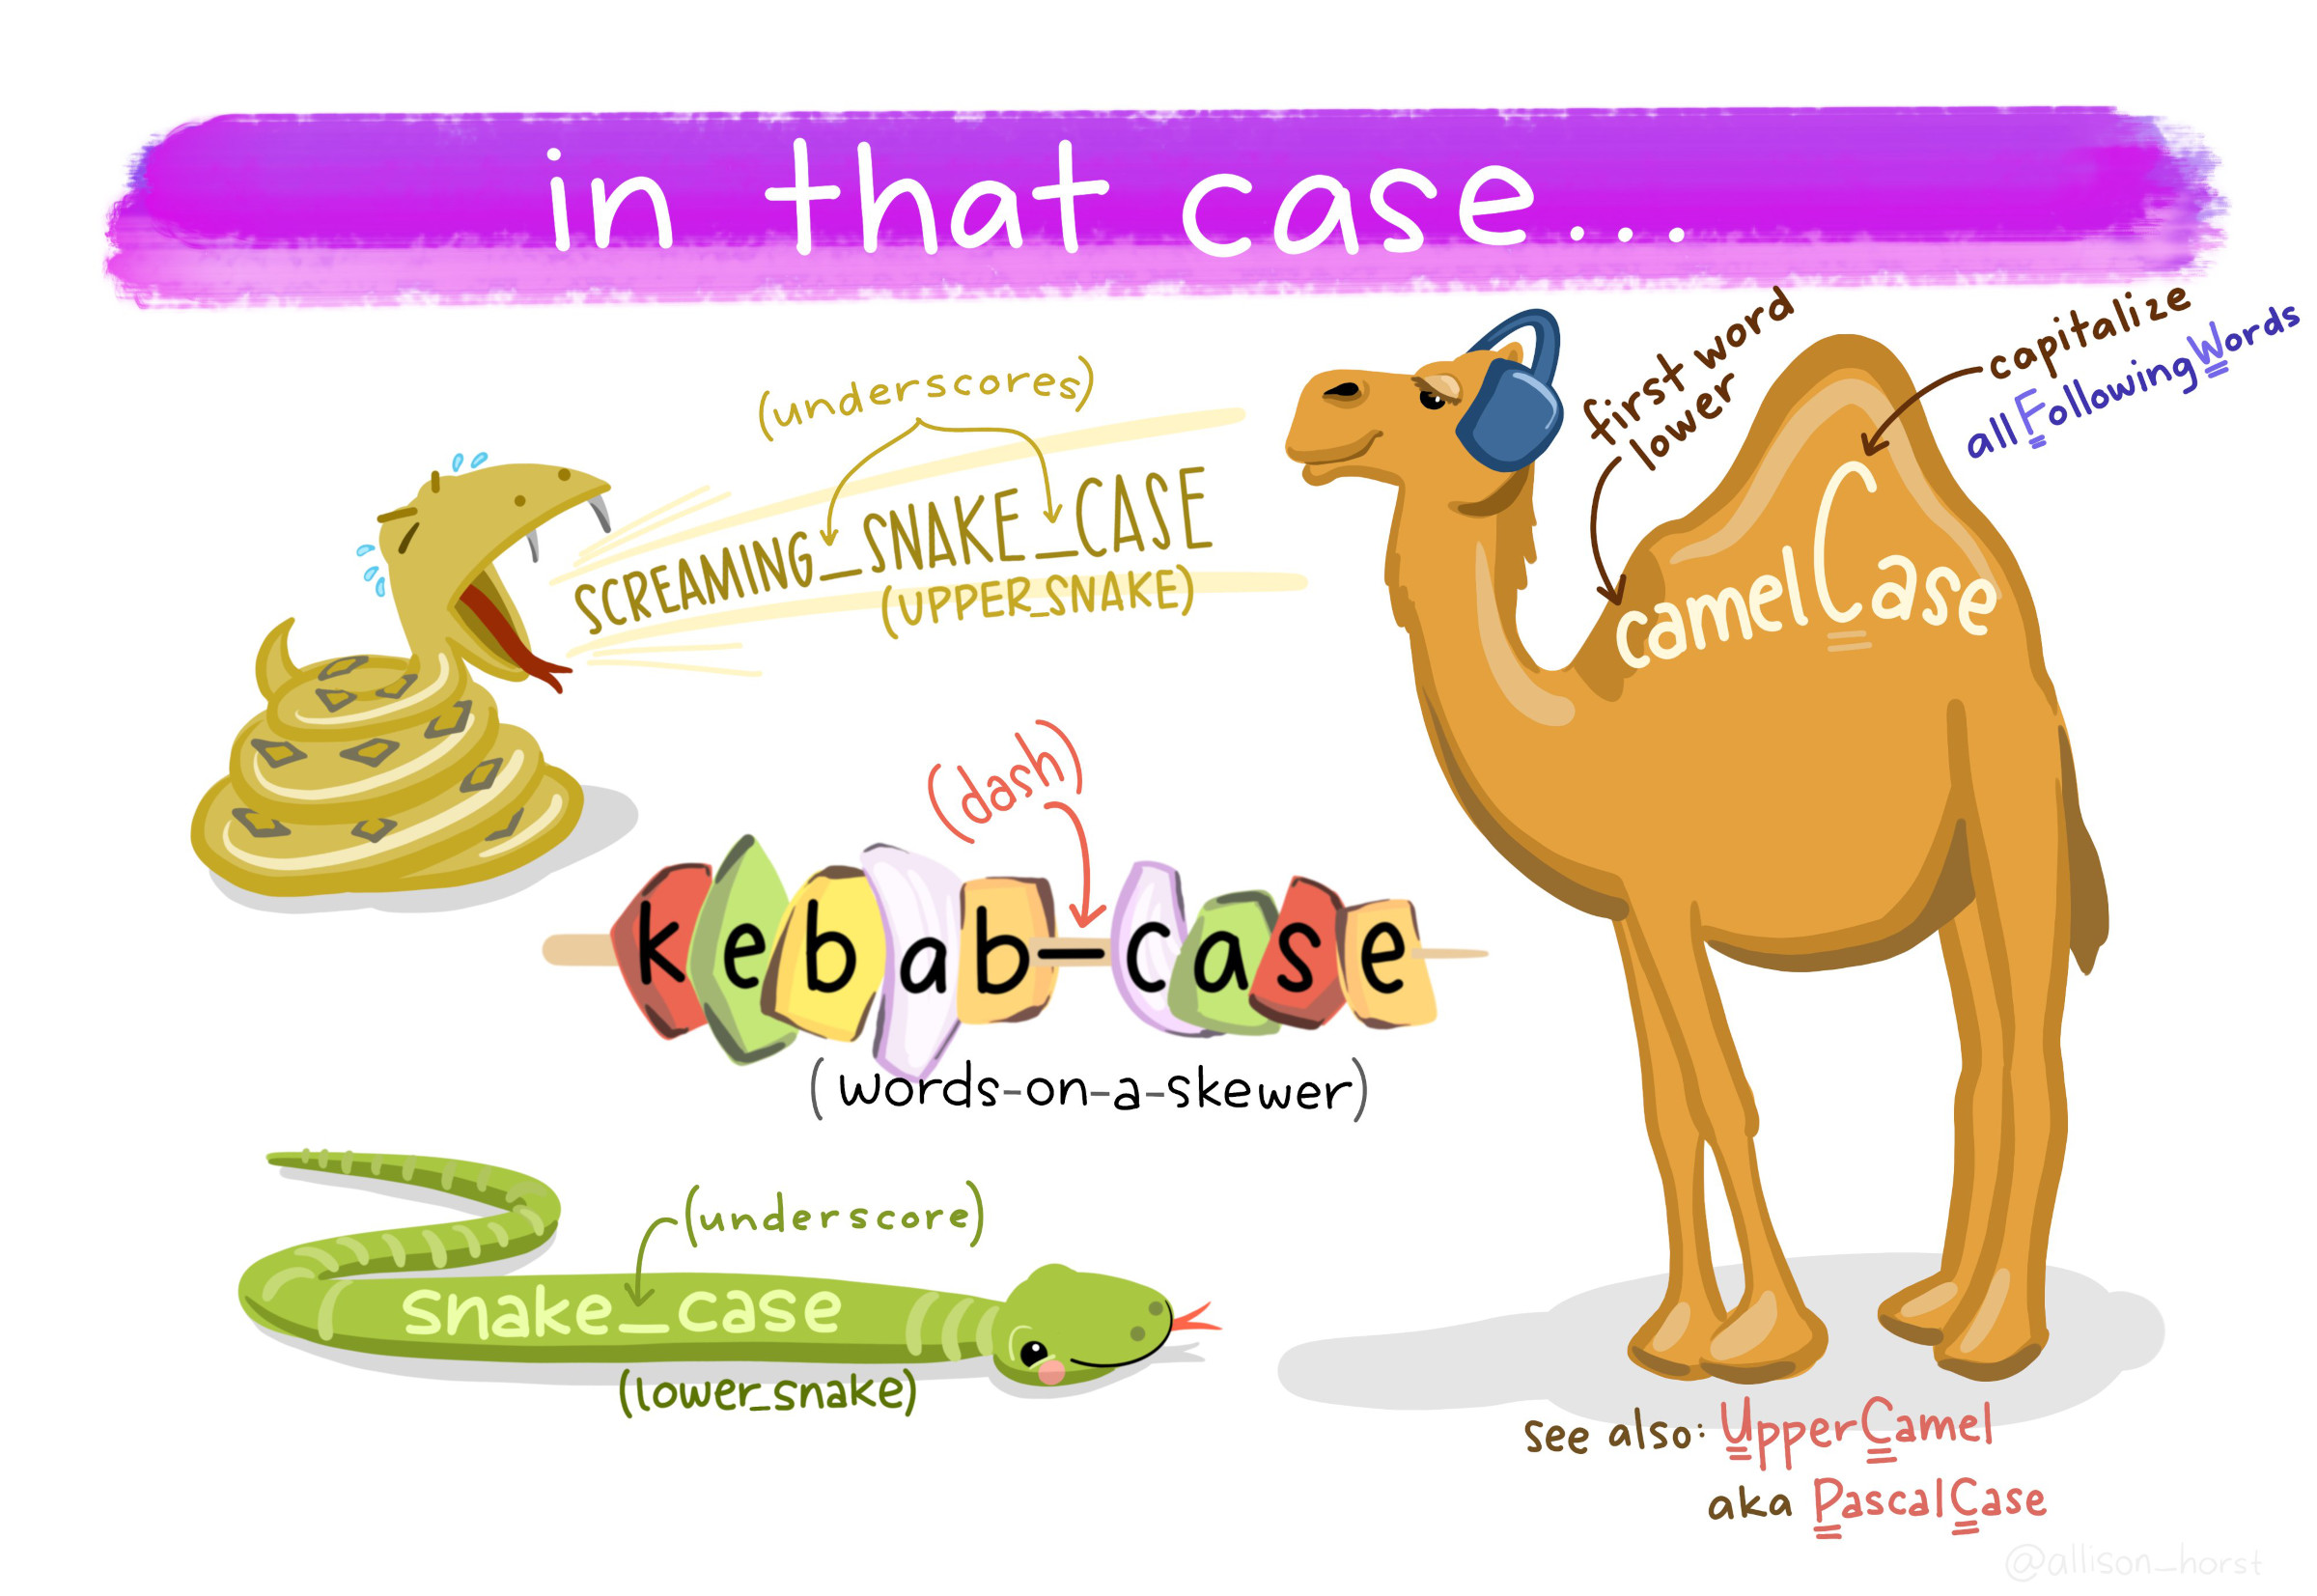
\includegraphics[width=0.75\linewidth]{images/case_horst} 

}

\caption{Types of font cases (L to R, clockwise): Screaming Snake Case, Camel Case, Upper Camel, Snake Case, Kebab Case. Art Credit: Dr. Allison Horst, UCSB}\label{fig:case}
\end{figure}

\begin{itemize}
\tightlist
\item
  Use dashes (-) or underscores (\_) to separate elements in a file name for \textbf{documents} (ex: \texttt{20231212\_CVMC\_CRCA01\_Proposal\_LCS.doc});
\item
  Always use the \href{https://www.iso.org/iso-8601-date-and-time-format.html}{ISO 8601} date format in file names: \textbf{YYYYMMDD}. For example, in the file name \emph{20230131\_DTLA\_RA.csv} January 31, 2023 is represented as \textbf{20230131};
\item
  Preserve the 3-letter file extension for application-specific codes of file format (e.g.~.doc, .xls, .mov, .tif);
\item
  With sequential numbering (e.g., 1, 2, 3, etc.), use leading zeros to accommodate multi-digit versions. For example, use 01-10 for 1-10, 001-100 for 1-100, and so on;
\item
  Name all files to reflect their content or function. For example, use names such as \texttt{tortoise\_count\_table.csv}, \texttt{manuscript.Rmd}, or \texttt{vegetation\_analysis.r}. Do \textbf{not} use general nomenclature with sequential numbers (e.g., \texttt{result1.csv}, \texttt{result2.csv}) or a location in a final manuscript (e.g., \texttt{fig\_3\_a.png}), since those numbers will almost certainly change as the project evolves;
\item
  Include versioning of file names where appropriate, indicating the version with \texttt{rev} the date (ex: CVMC\_CRCA01\_Proposal\_LCS\_rev20230131.doc).

  \begin{itemize}
  \tightlist
  \item
    this is a bit different from the standardized \textbf{date first} file naming. It is recommended to \textbf{avoid} \emph{starting} the filename with a version number .The CCB lab can set the versioning to \texttt{CVMC\_CRCA01\_Proposal\_LCS\_rev20230131.doc}, but for the final document, name it \texttt{20231212\_CVMC\_CRCA01\_Proposal\_LCS.doc}.
  \item
    \emph{Final copies of tabular data} should be stored as a copy without macros or formulas, in a non-proprietary format such as comma or tab separated values (.csv or .txt) \citep{Smithsonian_2021}.
  \end{itemize}
\item
  Order the elements in a file name in the most appropriate way to retrieve the record. For example,

  \begin{itemize}
  \tightlist
  \item
    file name with the date first,
  \item
    the project name or project location (acronyms are very helpful here) should be second,
  \item
    then the type of data or file (either RA or Report or Brochure),
  \item
    then version and/or author,
  \end{itemize}
\end{itemize}

\hypertarget{file-name-examples}{%
\subsection{File Name Examples}\label{file-name-examples}}

\begin{itemize}
\tightlist
\item
  Vegetation assessment data collected on February 17, 2017 at the Coachella Valley Stormwater Channel: \texttt{20170217\_CVStormwaterVAP.csv},
\item
  Coachella Valley Mountain Conservancy Climate Resistance \& Community Access Grant Program (Proposal No.~CRCA-01) proposal document authored by Lynn Sweet and finalized \& submitted on December 31, 2022: \texttt{20221231\_CVMC-CRCA01\_Proposal\_LCS.doc}
\item
  Journal articles: \texttt{2020\_Thorne\_VegetationRefugiaInformClimate-adaptiveLandManagement.pdf}.
\end{itemize}

\hypertarget{esri-file-naming-guidelines-unique-exceptions}{%
\subsection{ESRI File Naming Guidelines \& Unique Exceptions}\label{esri-file-naming-guidelines-unique-exceptions}}

When naming objects, folders, databases to be used by ESRI software, there are some unique considerations that contradict the above file naming guidelines!

\begin{itemize}
\item
  \textbf{Avoid long pathnames.}
  Try to ``flatten'' folder structures so that file pathnames under 128 characters. The absolute Windows pathname limit (MAXPATH) is 260 characters.
\item
  \textbf{Start with a letter.}
  \emph{Never} begin an ArcGIS object name (table, field, relationship class, mxd file, folder, etc) with a number or any other non-alpha character.
\item
  \textbf{No reserved words, aka common coding function words.}
  Avoid names that may conflict with SQL or other language's reserved words. For example: \texttt{OBJECTID}, \texttt{VALUE}, \texttt{COUNT}, \texttt{NOT}, \texttt{OR}, \texttt{ON}, \texttt{IN}, \texttt{OVER}, \texttt{SELECT}. This is to avoid confusing both people and SQL or Python or R.
\item
  \textbf{Be brief.}
  All field names should contain \textbf{10 characters or less}. This is a dBase limit, so it applies to .dbf files AND shapefiles. For that reason it's best practice in case you need to go ``through'' a dbf based format. Coverage and grid names have a limit of 13 characters, but 10 is safer. If you really want a longer name around or one with special characters, use the alias.
\item
  \textbf{Raster dataset names MUST start with a letter}
  Raster names can be particularly problematic and it is best to keep the filename \textbf{under 14 characters} to support Esri grid format, and special characters in the path (space, \&, -) may cause raster exports and tools to fail with cryptic error messages (like 999999).
\item
  \textbf{Use code in scripting to check names.}
  The arcpy methods \texttt{ValidateFieldName} and \texttt{ValidateTableName} can be used at parameter validation time, or in your code, to prevent users of your tool from inserting invalid output names. The \texttt{CreateScratchName} method if provided the proper arguments, will generate valid dataset names.
\end{itemize}

\hypertarget{directory-organization}{%
\section{Directory Organization}\label{directory-organization}}

The amount of data and files research organizations create and store has grown significantly due to technological advances in field data collection tools and open-source software. As the amount of data collected and reports generated increases, it is necessary to establish a clear, logical directory organization framework.

\hypertarget{recommendations-for-directory-organization}{%
\subsection{Recommendations for Directory Organization}\label{recommendations-for-directory-organization}}

The following recommendations were pulled from \citet{Spreckelsen_2020}.

\begin{enumerate}
\def\labelenumi{\arabic{enumi}.}
\tightlist
\item
  \textbf{Put each project in its own directory}
\end{enumerate}

Create a new folder for each new project and name that folder after the project. Some researchers create a separate project for each manuscript they are working on, while others group all research on a common theme or data set into a single project.
As a rule of thumb, divide work into projects based on the overlap in data and code files. If 2 research efforts share no data or code, they will probably be easiest to manage independently. If they share more than half of their data and code, they are probably best managed together, while if you are building tools that are used in several projects, the common code should probably be in a project of its own. Projects do often require their own organizational model, but below are general recommendations on how you can structure data, code, analysis outputs, and other files. The important concept is that it is useful to organize the project by the types of files and that consistency helps you effectively find and use things later.

\begin{enumerate}
\def\labelenumi{\arabic{enumi}.}
\setcounter{enumi}{1}
\tightlist
\item
  \textbf{Put text documents associated with the project in a `document' directory.}
\end{enumerate}

This includes files for manuscripts, documentation for source code, and/or an electronic lab notebook recording your experiments. Subdirectories may be created for these different classes of files in large projects. Create subdirectories within the \texttt{document} folder to account for the various types of documents required for each project. For example, does this project include pre-proposals for funding? If so, create a subfolder \texttt{proposal}. If the project is grant funded, create a \texttt{report} folder to save the various reports required for the funding.

\begin{enumerate}
\def\labelenumi{\arabic{enumi}.}
\setcounter{enumi}{2}
\tightlist
\item
  \textbf{Raw Data and Analysis Results}
\end{enumerate}

\begin{itemize}
\tightlist
\item
  \textbf{Put raw data and metadata in a \texttt{data} directory}
\end{itemize}

The data directory might require subdirectories to organize raw data based on time, method of collection, or other metadata most relevant to your analysis. These files should include the raw .xls and .csv files, plus additional .txt \& .md files.

\begin{itemize}
\tightlist
\item
  \textbf{Put files generated during cleanup and analysis in a \texttt{results} directory}
\end{itemize}

The \texttt{results} directory will usually require additional subdirectories for all but the simplest projects. \emph{Generated files} are considered intermediate files, such as cleaned data, statistical tables, and final publication-ready figures or tables and should be separated clearly by file-naming conventions or placed into different subdirectorie.

\begin{enumerate}
\def\labelenumi{\arabic{enumi}.}
\setcounter{enumi}{3}
\tightlist
\item
  \textbf{Put project source code in the \texttt{repository} directory.}
\end{enumerate}

The \texttt{respository}, also contains all of the code written for the project. This includes programs written in interpreted languages such as R or Python; as well as shell scripts, snippets of SQL used to pull information from databases; and other code needed to regenerate the results.
This directory may contain \textbf{two} conceptually distinct types of files that should be distinguished either by clear file names or by additional subdirectories.

\begin{itemize}
\tightlist
\item
  The first type is files or groups of files that perform the core analysis of the research, such as data cleaning or statistical analyses. These files can be thought of as the ``scientific guts'' of the project.
\item
  The second type of file in \texttt{respository} is controller or driver scripts that contain all the analysis steps for the entire project from start to finish, with particular parameters and data input/output commands. A controller script for a simple project, for example, may read a raw data table, import and apply several cleanup and analysis functions from the other files in this directory, and create and save a numeric result. For a small project with 1 main output and all the code is in R, save R files in a \texttt{R} folder.
\end{itemize}

\begin{enumerate}
\def\labelenumi{\arabic{enumi}.}
\setcounter{enumi}{4}
\tightlist
\item
  \textbf{Images and Visualizations}
\end{enumerate}

Photos, screenshots, and plots or other types of data visualizations should be saved in a separate \texttt{images} project sub-directory.

\begin{enumerate}
\def\labelenumi{\arabic{enumi}.}
\setcounter{enumi}{5}
\tightlist
\item
  \textbf{Put project scratch work and analysis in a \texttt{sandbox} directory.}
\end{enumerate}

Create a \texttt{sandbox} directory within the appropriate project folder for experimental project work. A \texttt{sandbox} folder is useful in a the \texttt{src} or \texttt{r} folder as it can serve as location to save test code or tutorials to conduct analysis.

\begin{enumerate}
\def\labelenumi{\arabic{enumi}.}
\setcounter{enumi}{6}
\tightlist
\item
  \textbf{Create an \texttt{archive} folder for out-of-date data or versions}
\end{enumerate}

An \texttt{archive} folder serves as a repository for long-term data retention. Data and reference materials stored in the \texttt{archive} folder are no longer the most relevant versions, but important reference files that should be preserved but not utilized for analysis.

\hypertarget{folder-organization-examples}{%
\subsection{Folder Organization Examples:}\label{folder-organization-examples}}

\begin{enumerate}
\def\labelenumi{\arabic{enumi})}
\tightlist
\item
  Data Analysis Project
\end{enumerate}

\textbf{Simple Project}

\begin{verbatim}
my-simple-project/
├── InputData          <- Folder containing data that will be processed
├── OutputData         <- Folder containing data that has been processed
├── Figures            <- Folder containing with figures or tables summarizing the results
├── Code               <- Folder the scripts or programs to do the analysis
├── LICENSE            <- File explaining the terms under which data/code is being made available
├── README.txt         <- File documenting the analysis, and (ideally) the purpose of each file.
\end{verbatim}

\textbf{Advanced Projects}

Many kinds of input data, documentation, and code.

\begin{verbatim}
my-advanced-project/
├── repository/
├── AUTHORS.md         <- File: List of people that contributed to the project (Markdown format)
├── LICENSE            <- File: Plain text file explaining the usage terms/license of the data/code file (CC-By, MIT, GNU, etc.)
├── README.md          <- File: Readme file (Markdown format)
├── bin                <- Folder: Your compiled model code can be stored here (not tracked by git)
├── config             <- Folder: Configuration files, e.g., for doxygen or for your model if needed
├── data               <- Folder: Data for this project
│   ├── external       <- Folder: Data from third party sources.
│   ├── interim        <- Folder: Intermediate data that has been transformed.
│   ├── processed      <- Folder: The final, canonical data sets for modeling.
│   └── raw            <- Folder: The original, immutable data dump.
├── docs               <- Folder: Documentation, e.g., doxygen or scientific papers (not tracked by git)
├── notebooks          <- Folder: Ipython or R notebooks
├── reports            <- Folder: Manuscript source, e.g., LaTeX, Markdown, etc., or any project reports
│   └── figures        <- Folder: Figures for the manuscript or reports
└── src                <- Folder: Source code for this project
    ├── R           <- Folder: scripts and programs to process data
    ├── external       <- Folder: Any external source code, e.g., other projects, or external libraries
    ├── models         <- Folder: Source code for your own model
    ├── tools          <- Folder: Any helper scripts go here
    └── visualization  <- Folder: Visualisation scripts, e.g., matplotlib, ggplot2 related
\end{verbatim}

\begin{verbatim}
my-advanced-project_002/
├── repository/
│   ├── images/
│   │   ├── image-01.jpg
│   │   └── image-02.jpg
│   ├── templates/
│   │   ├── page.html
│   │   └── post.html
│   └── index.html
|   |── r/
│   |   ├── function.r
|   |   ├── analysis.r
|   |   ├── report.Rmd
│   ├── data/
│   |   ├── function.r
│   |   ├── function.r
│   ├── myproject.Rproj
└── README.md
\end{verbatim}

\begin{enumerate}
\def\labelenumi{\arabic{enumi})}
\setcounter{enumi}{1}
\tightlist
\item
  Vegetation Monitoring Project
\end{enumerate}

\begin{verbatim}
vegetation/
DesertTortoiseLinkageArea/
├── images/
│   ├── RelevePlots
│   │   ├── DTLA_plot001-01.jpg
│   │   └── DTLA_plot001-02.jpg
│   ├── PlantId
│   │   ├── AlloniaIncarnata_BerdooCyn_2022-001.jpg
│   │   └── AlloniaIncarnata_BerdooCyn_2022-002.jpg
├── repositories/
│   ├── DTLA
│   │   │── r/
│   │   │   ├── function.r
│   │   │   ├── analysis.r
│   │   │   ├── report.Rmd
│   │   ├── data/
│   │   │   ├── data.csv
│   │   │   ├── data.csv
│   │   ├── myproject.Rproj
│   │   ├── README.md
├── documents/
│   ├── DTLA
│   │   │── _archive/
│   │   │   │── geodatabase/
│   │   │   │── report_drafts/
│   │   │── reports/
│   │   │   ├── 2021AnnualReport.doc
│   │   │   ├── 2021AnnualReport.doc
│   │   │   ├── 2021AnnualReport.doc
│   │── reference/
│   │   │── CNPS_RapidAssessmentProtocol/
│   │   │   ├── 2017_CNPSRapidAssessmentProtocol.pdf
│   │   │   ├── 2018_CNPSRapidAssessmentProtocol.pdf
│   │   │   ├── 2020_CNPSRapidAssessmentProtocol.pdf
│   │   │── Species/
│   │   │   ├── PlantIdentificationGuides
│   │   │   │   ├── 2022_JOTRSpeciesGuide.pdf
│   │   │   ├── SpeciesInformation
│   │   │   │   ├── AlloniaIncarnata
│   │   │   │   │   ├── AlloniaIncarnataSpeciesInfo.pdf
└── recycle/
\end{verbatim}

\hypertarget{additional-resources}{%
\subsection{Additional Resources}\label{additional-resources}}

\begin{itemize}
\tightlist
\item
  \href{https://web.stanford.edu/~gentzkow/research/CodeAndData.pdf}{Gentzkow M, Shapiro JM. Code and Data for the Social Sciences: A Practitioner's Guide; 2014}. \url{https://web.stanford.edu/~gentzkow/research/CodeAndData.pdf}.
\item
  \href{https://academic.oup.com/bioscience/article/67/6/546/3784601}{Hampton S.E, et al.~Skills and Knowledge for Data-Intensive Environmental Research. BioScience, Volume 67, Issue 6, June 2017, Pages 546--557.}
\item
  \href{https://journals.plos.org/ploscompbiol/article?id=10.1371/journal.pcbi.1000424}{Noble WS. A Quick Guide to Organizing Computational Biology Projects. PLoS Comput Biol. 2009;5(7).}
\end{itemize}

\hypertarget{data-management}{%
\section{Data Management}\label{data-management}}

\citet{Wilson_2017} recommend following these data management practices:

\begin{itemize}
\tightlist
\item
  Save the raw data.
\item
  Ensure that raw data are backed up in more than one location.
\item
  Create the data you wish to see in the world.
\item
  Create analysis-friendly data.
\item
  Record all the steps used to process data.
\item
  Anticipate the need to use multiple tables, and use a unique identifier for every record.
\item
  Submit data to a reputable DOI-issuing repository so that others can access and cite it (ex: \href{https://www.dataone.org/}{DataOne}, \href{https://knb.ecoinformatics.org/}{KNB}, and \href{https://www.ncei.noaa.gov/access/search/index}{NCEI}.
\end{itemize}

\hypertarget{tidy-data}{%
\subsection{Tidy Data}\label{tidy-data}}

\textbf{Tidy data} is one of the most important concepts for any data scientist. It provides predictable organization for data that makes coding, analysis, and collaboration easier.

Tidy data satisfies the following conditions:

\begin{itemize}
\tightlist
\item
  Each observation is in a row
\item
  Each variable in a column
\item
  Each value is in a single cell
\end{itemize}

\begin{figure}

{\centering 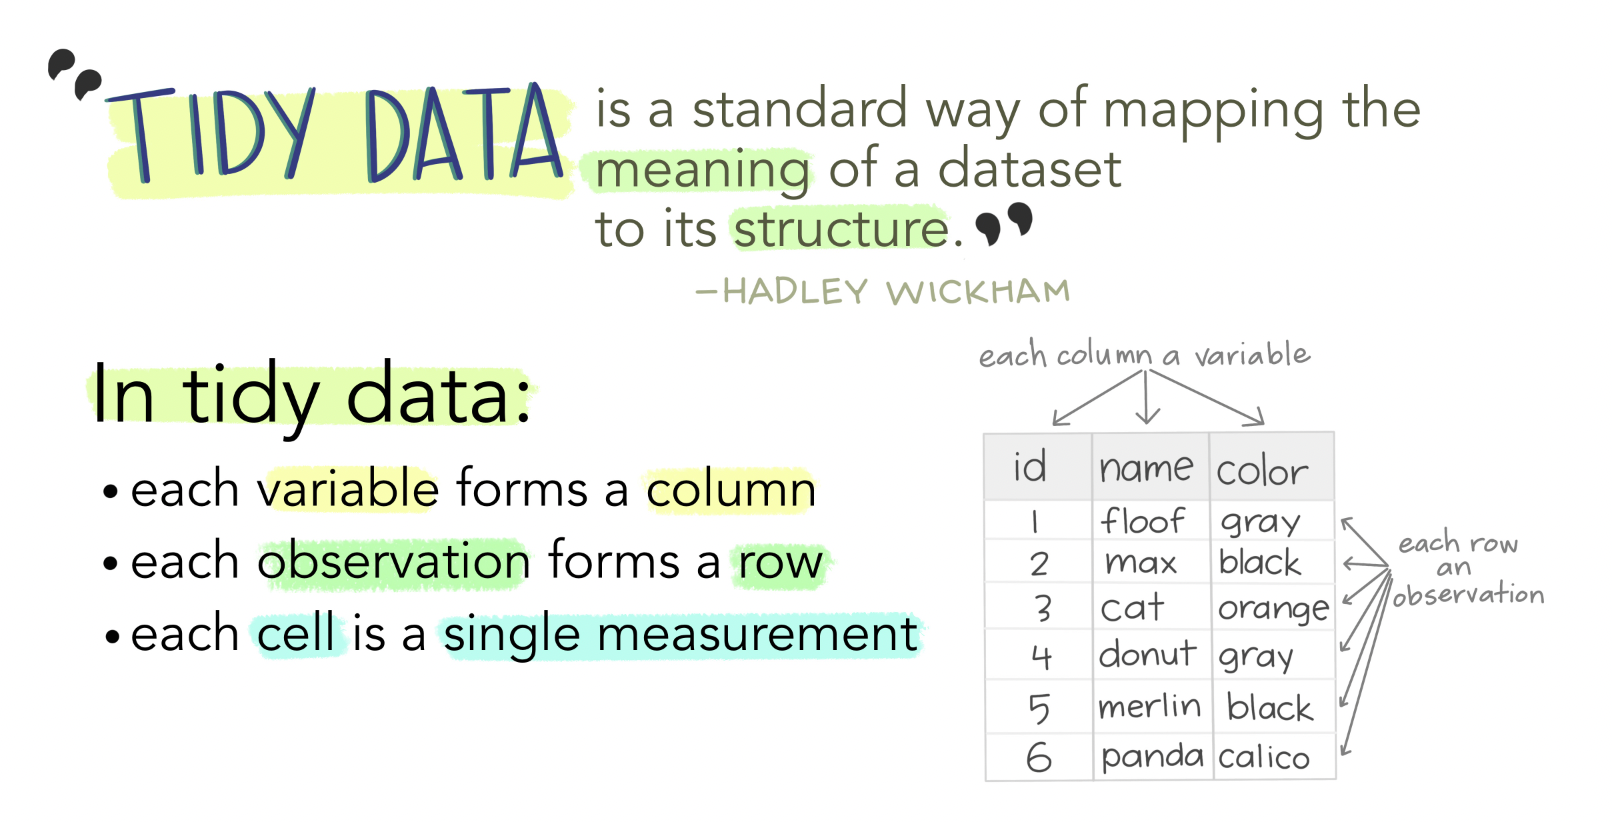
\includegraphics[width=0.9\linewidth]{images/tidydata_horst} 

}

\caption{Tidy data allows for efficient data science, easy collaboration, and ensures reproducibility and reuse. Art Credit: Dr. Allison Horst, UCSB}\label{fig:tidydata}
\end{figure}

\citet{Broman_2018} state the core principles for tidy data are:

\begin{itemize}
\tightlist
\item
  be consistent with data collection and entry,
\item
  write dates like YYYY-MM-DD,
\item
  don't leave any cells empty,
\item
  put just one thing in a cell,
\item
  organize the data as a single rectangle

  \begin{itemize}
  \tightlist
  \item
    with subjects as rows and variables as columns,
  \item
    and with a single header row,
  \end{itemize}
\item
  create a data dictionary,
\item
  don't include calculations in the raw data files,
\item
  don't use font color or highlighting as data,
\item
  choose good names for things,
\item
  make backups,
\item
  use data validation to avoid data entry errors,
\item
  and save the data in \textbf{plain text files} (i.e.~.csv, .txt).
\end{itemize}

The R package, \texttt{tidyverse}, is one of the best tools to tidy data! The tidyverse is an opinionated collection of R packages designed for data science. All packages share an underlying design philosophy, grammar, and data structures.

Install the complete tidyverse with:

\begin{Shaded}
\begin{Highlighting}[]
\FunctionTok{install.packages}\NormalTok{(}\StringTok{"tidyverse"}\NormalTok{)}
\end{Highlighting}
\end{Shaded}

Then load the \textbf{tidyverse} package in a code chunk with the command:

\begin{Shaded}
\begin{Highlighting}[]
\FunctionTok{library}\NormalTok{(tidyverse)}
\end{Highlighting}
\end{Shaded}

The packages contained within the \href{https://www.tidyverse.org/packages/}{\textbf{tidyverse}} are:

\begin{itemize}
\tightlist
\item
  \href{https://ggplot2.tidyverse.org/}{ggplot2} is a system for creating graphics for your data, based on The Grammar of Graphics. Plot your data with ggplot2!
\item
  \href{https://dplyr.tidyverse.org/}{dplyr} is a data manipulation package that provides a consistent set of verbs to manipilate data:

  \begin{itemize}
  \tightlist
  \item
    \texttt{mutate()} adds new variables that are functions of existing variables
  \item
    \texttt{select()} picks variables based on their names.
  \item
    \texttt{filter()} picks cases based on their values.
  \item
    \texttt{summarise()} reduces multiple values down to a single summary.
  \item
    \texttt{arrange()} changes the ordering of the rows.
  \end{itemize}
\item
  \href{https://tidyr.tidyverse.org/}{tidyr} is the tidying data workhorse package within the \textbf{tidyverse}. Use \textbf{tidyr} to wrangle, pivot, and convert or replace missing data.
\item
  \href{https://readr.tidyverse.org/}{readr} is a fast way to read rectangular data from delimited files, such as comma-separated values (CSV) and tab-separated values (TSV).
\item
  \href{https://purrr.tidyverse.org/}{purrr} provides a complete and consistent set of tools for working with functions and vectors.
\item
  \href{https://tibble.tidyverse.org/}{tibble} is a version of \texttt{data.frame}, but they do less (i.e.~they don't change variable names or types, and don't do partial matching) and complain more (e.g.~when a variable does not exist).
\item
  \href{https://stringr.tidyverse.org/}{stringr} provides a cohesive set of functions designed to make working with strings as easy as possible.
\item
  \href{https://forcats.tidyverse.org/}{forcats} provides a suite of tools that solve common problems with factors, including changing the order of levels or the values.

  \begin{itemize}
  \tightlist
  \item
    \texttt{fct\_reorder()}: Reordering a factor by another variable.
  \item
    \texttt{fct\_infreq()}: Reordering a factor by the frequency of values.
  \item
    \texttt{fct\_relevel()}: Changing the order of a factor by hand.
  \item
    \texttt{fct\_lump()}: Collapsing the least/most frequent values of a factor into ``other''.
  \end{itemize}
\end{itemize}

\begin{figure}

{\centering 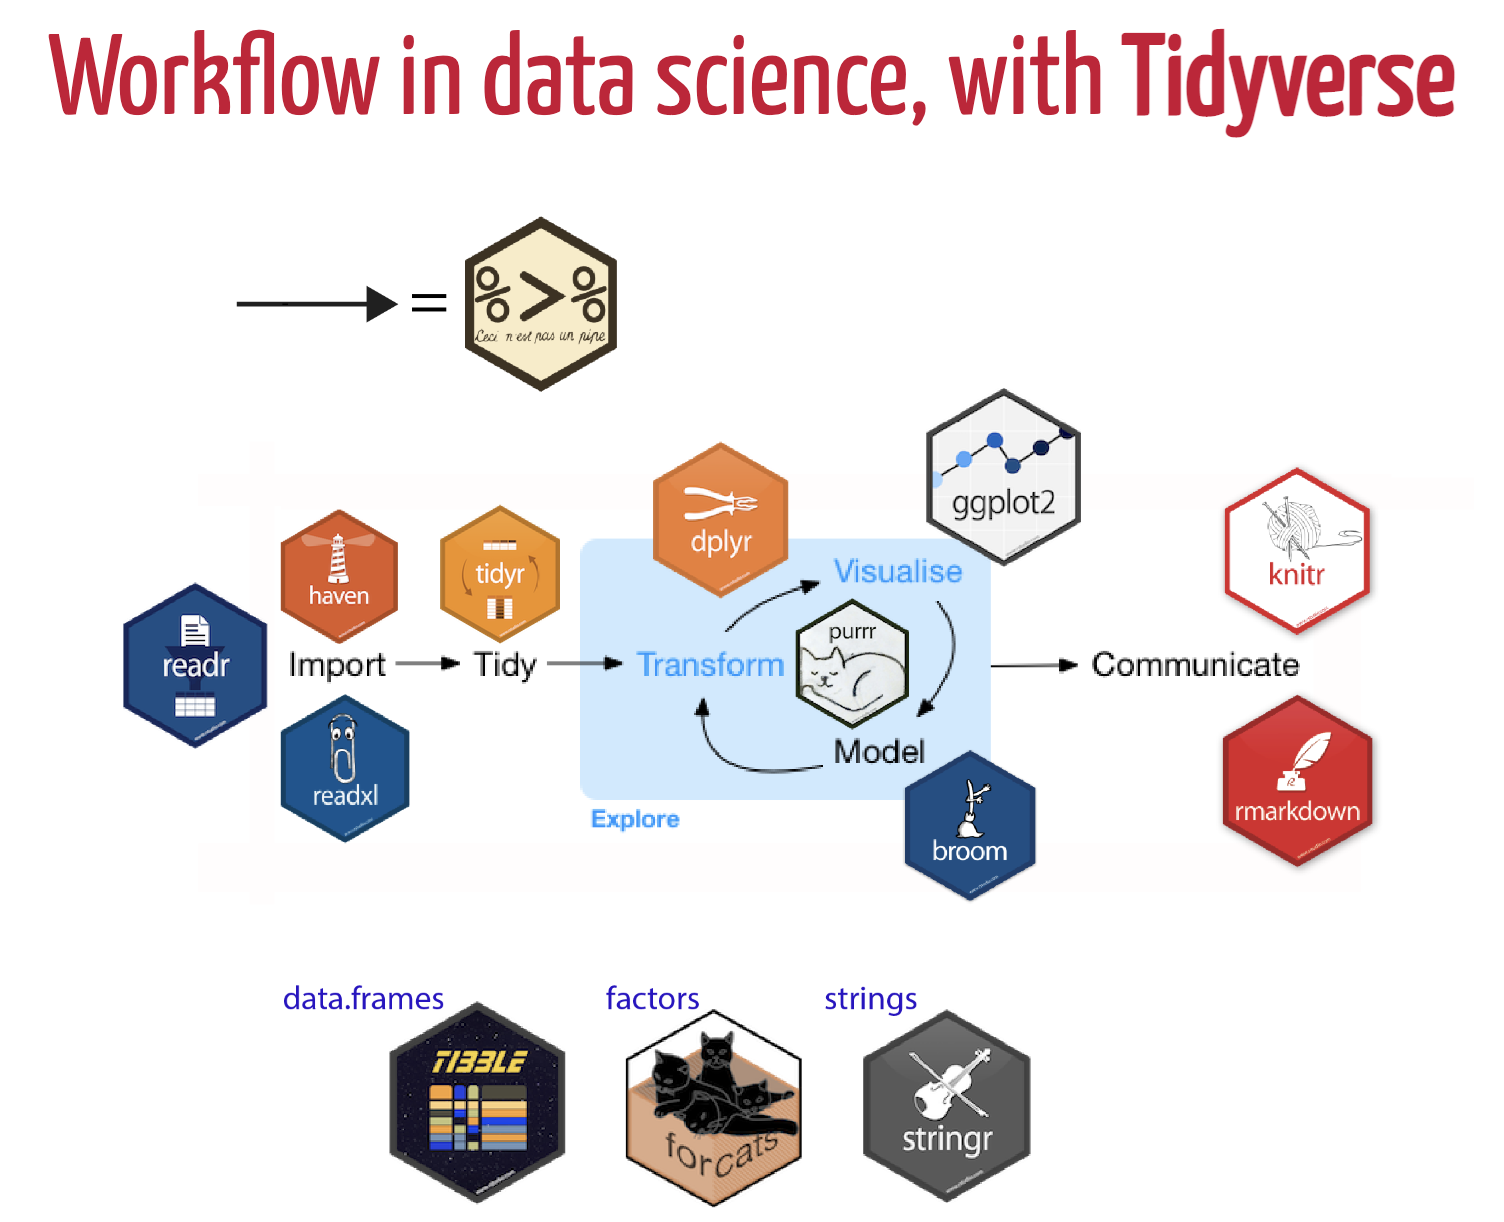
\includegraphics[width=1\linewidth]{images/tidyverse} 

}

\caption{Data Science workflow utilizing Tidyverse packages. Art Credit: Dr. Olivier Gimenez}\label{fig:tidyverse}
\end{figure}

\hypertarget{project-development-and-collaboration}{%
\subsection{Project Development and Collaboration}\label{project-development-and-collaboration}}

The foundation of developing and organizing a project is to design it to make it easy for new collaborators to join and for current coworkers to collaborate seemlessly. This involves making it easy for people to set up a local workspace so that they can contribute, help them find what to contribute, and make the organization process clear so that they know how to contribute.

Steps to consider when developing a research project:

\begin{enumerate}
\def\labelenumi{\arabic{enumi}.}
\tightlist
\item
  \textbf{Create an overview of your project.}
\end{enumerate}

Have a short file in the project's home directory that explains the purpose of the project. This file (generally README.txt or README.md) should contain the project's:

\begin{itemize}
\tightlist
\item
  title,
\item
  a brief description,
\item
  up-to-date contact and/or author information,
\item
  and an example or 2 of how to run various cleaning or analysis tasks,
\item
  describes what is needed for the project and use or contribute to it, i.e., dependencies that need to be installed, tests that can be run to ensure that software has been installed correctly, and guidelines or checklists that the project adheres to.
\end{itemize}

It is often the first thing users and collaborators on your project will look at, so make it explicit how you want people to engage with the project.

\begin{enumerate}
\def\labelenumi{\arabic{enumi}.}
\setcounter{enumi}{1}
\tightlist
\item
  \textbf{Create a shared ``to-do'' list.}
\end{enumerate}

This can be a plain text file called something like notes.txt or todo.txt, or utilize GitHub project management tools to create a new issue for each to-do item. Describe the items clearly so that the tasks are clear and easily understood.

\begin{enumerate}
\def\labelenumi{\arabic{enumi}.}
\setcounter{enumi}{2}
\tightlist
\item
  \textbf{Decide on communication strategies.}
\end{enumerate}

Make explicit decisions about (and publish where appropriate) how members of the project will communicate with each other and with externals users/collaborators. This includes the location and technology for email lists, chat channels, voice/video conferencing, documentation, and meeting notes, as well as which of these channels will be public or private.

\begin{enumerate}
\def\labelenumi{\arabic{enumi}.}
\setcounter{enumi}{3}
\tightlist
\item
  \textbf{Make the license explicit.}
\end{enumerate}

Create a LICENSE file in the project's home directory that clearly states what license(s) apply to the project's software, data, and manuscripts. The one most frequently recommended is the \textbf{Creative Common} licenses for data and text.

\begin{enumerate}
\def\labelenumi{\arabic{enumi}.}
\setcounter{enumi}{4}
\tightlist
\item
  \textbf{Ensure the project is citable.}
\end{enumerate}

Include a \texttt{CITATION} file in the project's home directory that describes how to cite this project as a whole and where to find (and how to cite) any data sets, code, and figures. Below is an example \texttt{CITATION} file for the Ecodata Retriever (\url{https://github.com/weecology/retriever}):

\texttt{Please\ cite\ this\ work\ as:\ Morris,\ B.D.\ and\ E.P.\ White.\ 2013.\ "The\ EcoData\ Retriever:\ improving\ access\ to\ existing\ ecological\ data".\ PLoS\ ONE\ 8:e65848.}

\emph{Guidance above taken from \citet{Wilson_2017}.}

\hypertarget{fair-data-management-principles}{%
\subsection{FAIR Data Management Principles}\label{fair-data-management-principles}}

In 2016, the \textbf{FAIR Guiding Principles for scientific data management and stewardship} were published in \emph{Scientific Data}. The authors intended to provide guidelines to improve the \textbf{F}indability, \textbf{A}ccessibility, \textbf{I}nteroperability, and \textbf{R}euse of digital assets \citep{Wilkinson_2016}.

In this article, the authors outline the \textbf{FAIR} Guiding Principles as:

\begin{enumerate}
\def\labelenumi{\arabic{enumi}.}
\tightlist
\item
  To be \textbf{F}indable:

  \begin{itemize}
  \tightlist
  \item
    F1. (meta)data are assigned a globally unique and persistent identifier
  \item
    F2. data are described with rich metadata (defined by R1 below)
  \item
    F3. metadata clearly and explicitly include the identifier of the data it describes
  \item
    F4. (meta)data are registered or indexed in a searchable resource
  \end{itemize}
\item
  To be \textbf{A}ccessible:

  \begin{itemize}
  \tightlist
  \item
    A1. (meta)data are retrievable by their identifier using a standardized communications protocol

    \begin{itemize}
    \tightlist
    \item
      A1.1 the protocol is open, free, and universally implementable
    \item
      A1.2 the protocol allows for an authentication and authorization procedure, where necessary
    \end{itemize}
  \item
    A2. metadata are accessible, even when the data are no longer available
  \end{itemize}
\item
  To be \textbf{I}nteroperable:

  \begin{itemize}
  \tightlist
  \item
    I1. (meta)data use a formal, accessible, shared, and broadly applicable language for knowledge representation.
  \item
    I2. (meta)data use vocabularies that follow FAIR principles
  \item
    I3. (meta)data include qualified references to other (meta)data
  \end{itemize}
\item
  To be \textbf{R}eusable:

  \begin{itemize}
  \tightlist
  \item
    R1. meta(data) are richly described with a plurality of accurate and relevant attributes

    \begin{itemize}
    \tightlist
    \item
      R1.1. (meta)data are released with a clear and accessible data usage license
    \item
      R1.2. (meta)data are associated with detailed provenance
    \item
      R1.3. (meta)data meet domain-relevant community standards
    \end{itemize}
  \end{itemize}
\end{enumerate}

\hypertarget{additional-resources-1}{%
\subsection{Additional Resources}\label{additional-resources-1}}

For more information on tidy data and data management:

\begin{itemize}
\tightlist
\item
  Julia Lowndes \& Allison Horst's \href{https://www.openscapes.org/blog/2020/10/12/tidy-data/}{Tidy Data blog}
\item
  Hadley Wickham \href{https://vita.had.co.nz/papers/tidy-data.pdf}{Tidy Data}
\item
  Grolemund \& Wickham \href{https://r4ds.had.co.nz/}{R for Data Science}
\item
  Lowndes, J.S., et al.~\href{https://www.nature.com/articles/s41559-017-0160}{Our Path to Better Science in Less Time Using Open Data Science Tools.}
\end{itemize}

\hypertarget{equipment}{%
\chapter{Equipment}\label{equipment}}

Inventory of software and equipment used and references

\begin{itemize}
\item
  ARC MAP DESKTOP: ArcMap ArcGIS Desktop, version 10.9 (Esri, Redlands, California)
\item
  LASER RANGEFINDER: Hilti PD-42 laser rangefinder (Hilti Corporation, Schaan, Liechtenstein)
\item
  TABLETS: Samsung Galaxy Tab Active 2 tablet (Samsung Group, Seoul, South Korea)
\item
  GPS: Trimble Juno 3
\item
  SERVER:

  \begin{itemize}
  \tightlist
  \item
    NAS model -- Synology DS920+
  \item
    Storage -- HUS728T8TALE6L4 Ultrastar DC HC320 8TB (x2, one for backup)
  \item
    OS \& Monitoring software -- Synology DSM (DiskStation Manager) 7.1-42661
  \end{itemize}
\end{itemize}

\hypertarget{concur}{%
\chapter{Concur Travel}\label{concur}}

UCR provides reimbursements for travel, lodging, and meals associated with travel for work. All travel must be discussed and approved by the PI (Lynn Sweet)

The new Concur Travel system has a modern, mobile-friendly user interface with built-in business rules to check for completeness prior to submitting an Expense Report. Please remember that, even though the travel application is changing, the UC travel policy is not and the Expense Report in the new Concur Travel system will still require a business purpose and itemized receipts for travel expenses. And, similar to the old iTravel system, the new Concur Travel system will allow only the Traveler to approve a Declaration of Missing Evidence (DME) and \emph{only} the Traveler can submit an Expense Report.

The new Concur Travel system uses a two-step process:

1 - Submitting a Trip Request prior to travelling

2 - Submitting an Expense Report after your trip is complete (Please note that BMPN Travel Arrangers can assist with training for this step)

\emph{Note} You can reach out to the BMPN Travel Arrangers (Sarah Acrey, Jeanette Westbrook, or Elisha Hankins) for assistance in completing your first Expense Report in Concur Travel. Please also note that at this time travel arrangers are not made aware when a trip has been requested or expense report submitted. While campus works to create a report, I ask that you please send a quick email to \href{mailto:BMPNPurchasing@ucr.edu}{\nolinkurl{BMPNPurchasing@ucr.edu}} to notify us that you have a travel pending review to prevent delays in processing.

\hypertarget{submitting-a-trip-request---before-the-trip}{%
\section{\texorpdfstring{Submitting a Trip Request - \emph{Before the trip}}{Submitting a Trip Request - Before the trip}}\label{submitting-a-trip-request---before-the-trip}}

First, you will need to log into the Concur Travel system.

-Log into your UCR Portal - \url{https://portal.ucr.edu/}.

-Navigate to Authorized Apps, then select the icon for Concur Travel and Expense.

-Log in with your verified UCR email address, the one associated with your UCR account, and sign in with university credentials

\hypertarget{make-a-trip-request-profile}{%
\subsection{Make a Trip Request Profile}\label{make-a-trip-request-profile}}

-Select \emph{Requests} on the upper right of the home page

-Select \emph{Create New Requests} in the center of the page

-Fill out the appropriate information for the request

-Click \emph{Create New Request}

\begin{flushleft}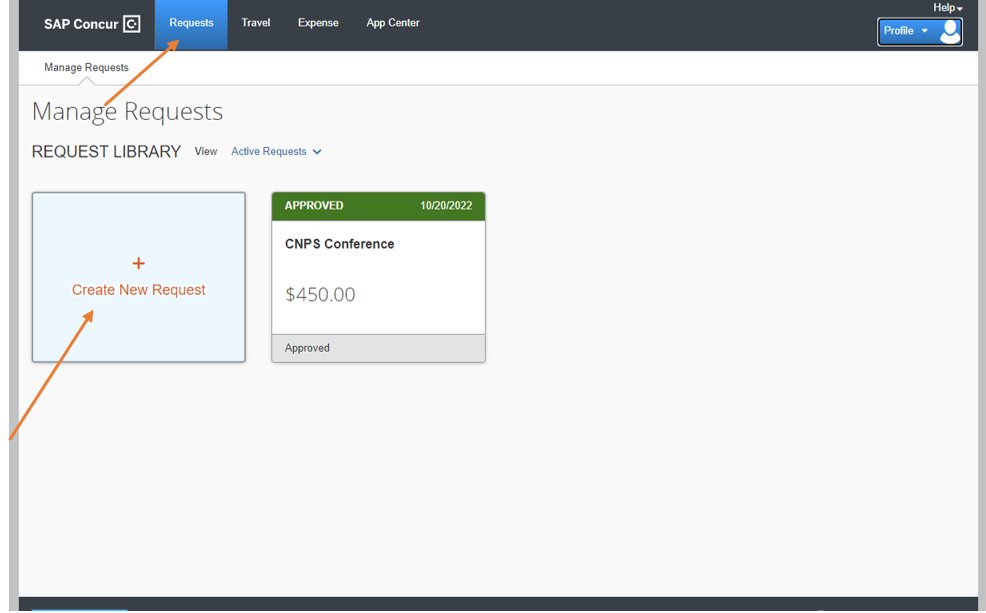
\includegraphics[width=0.75\linewidth]{images/concur1} \end{flushleft}

\emph{IMPORtANT NOTE}

-Trip Name must follow this format: Request ID - Travel start date - Travel end date (ex 34kf -- 082822 -- 090122). If you cannot find the Request ID, you can add it to the name after you have made the request under the title

-`Fund' is the FAU number. For the appropriate FAU see the Trello tab with current codes

-Cost center might change based on projects (\emph{NTCB} is for projects where Cam was the PI when they were created and \emph{NTLS} is for projects where Lynn is the PI),

-Approver ID is `Christine Morgando'.

\begin{flushleft}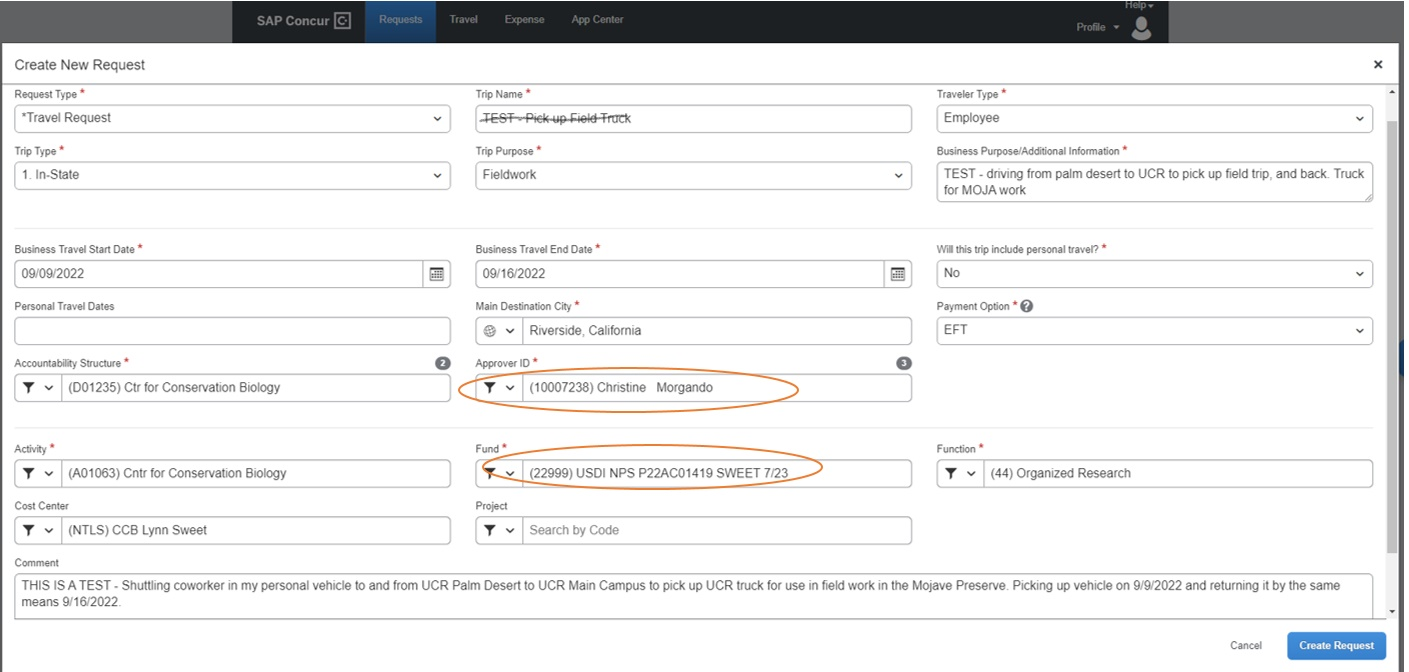
\includegraphics[width=0.75\linewidth]{images/concur2a} \end{flushleft}

\hypertarget{adding-expenses-to-the-trip-request}{%
\subsection{Adding Expenses to the Trip Request}\label{adding-expenses-to-the-trip-request}}

-Select the \emph{Add} button under Expected Expenses

\begin{flushleft}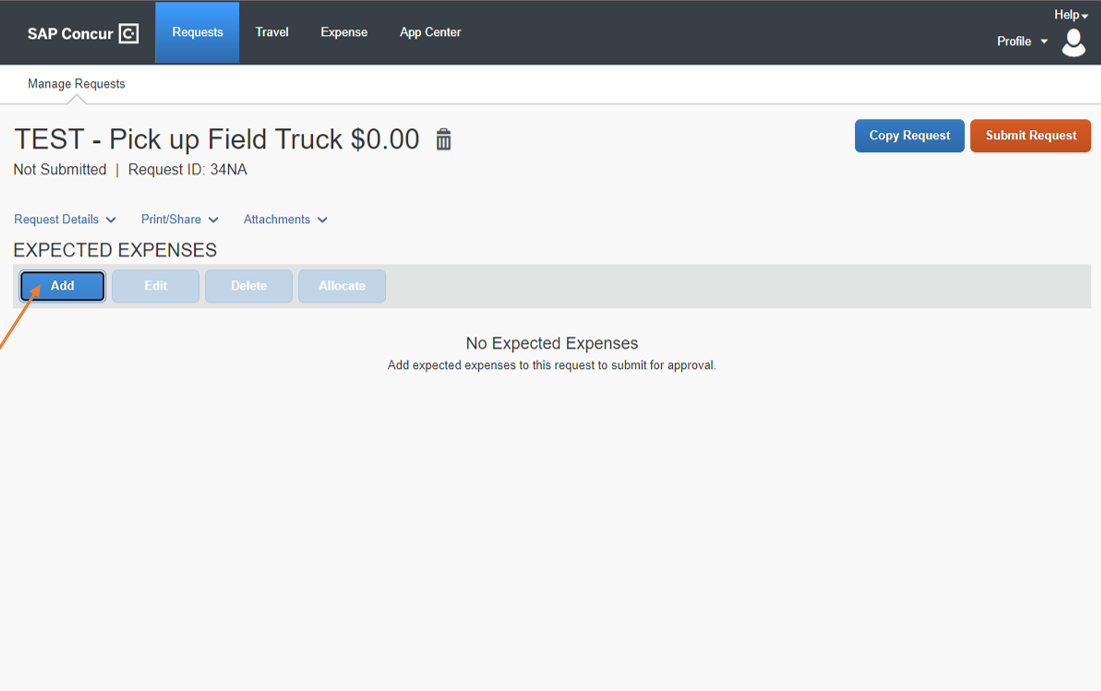
\includegraphics[width=0.75\linewidth]{images/concur3} \end{flushleft}

-Select \emph{Ground Transportation} (or any other \emph{expected} expenses such as food, lodging, registrations, etc.)

\begin{flushleft}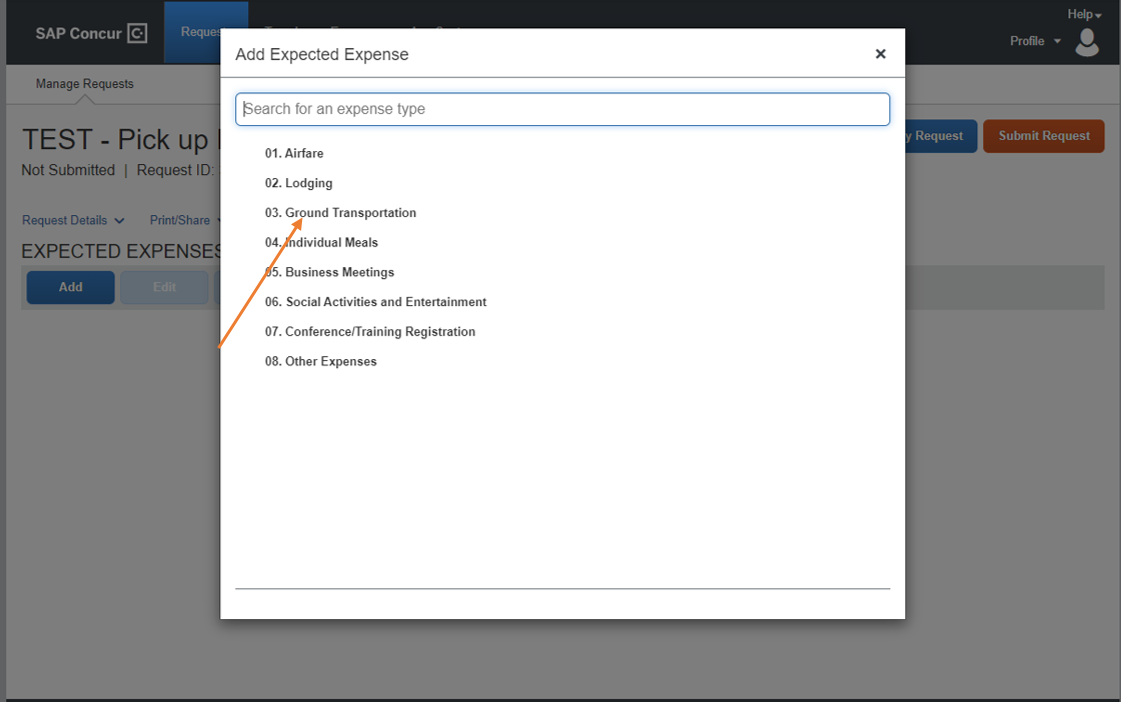
\includegraphics[width=0.75\linewidth]{images/concur4} \end{flushleft}

-Create a \emph{New Expense} for the trip

-Fill out the page with estimated amounts you expect for that category and Save
\emph{NOTE: MILEAGE REIBURSEMENT RATE HAS CHANGED, CURRENT RATES CAN BE FOUND {[}HERE{]} (\url{https://accounting.ucr.edu/travel-entertainment/mileage-reimbursement-rates})}

\begin{flushleft}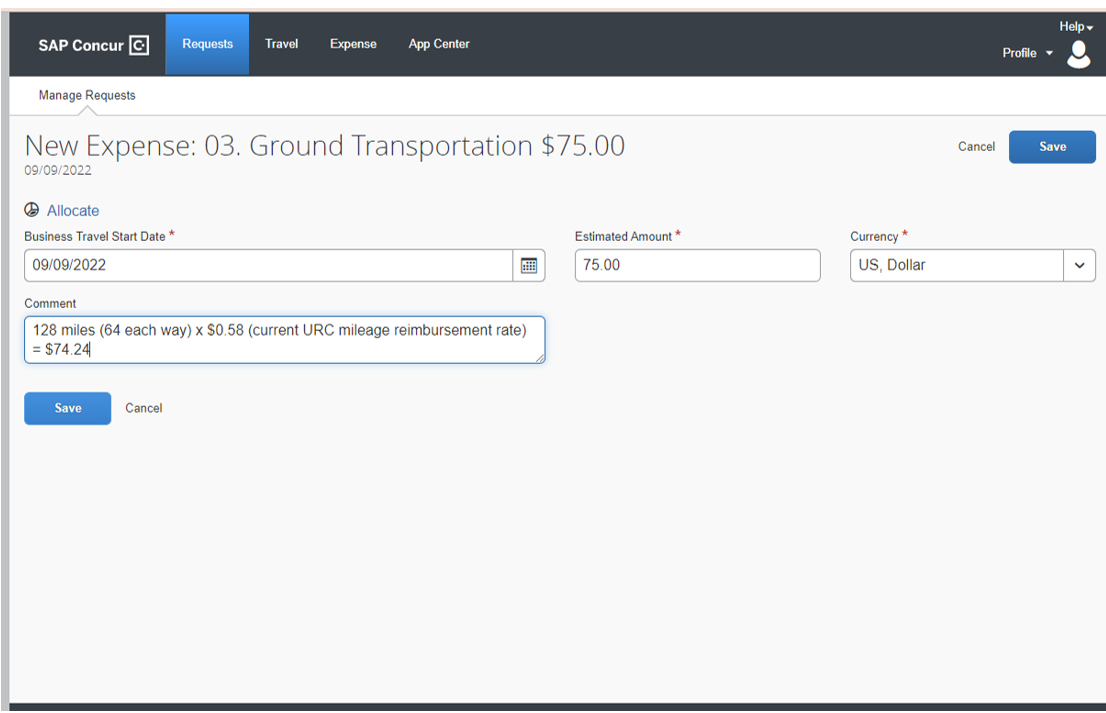
\includegraphics[width=0.75\linewidth]{images/concur5} \end{flushleft}

-Continue adding expected expenses until you've covered your bases, and then submit request.

\begin{flushleft}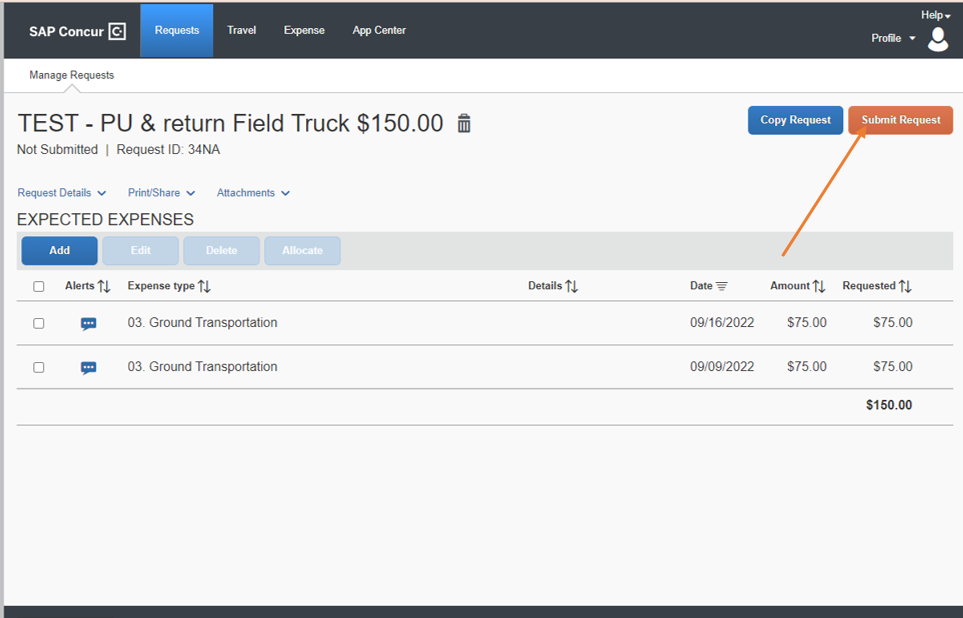
\includegraphics[width=0.75\linewidth]{images/concur6} \end{flushleft}

-Email Debbie Brown (\href{mailto:debbie.brown@ucr.edu}{\nolinkurl{debbie.brown@ucr.edu}}) with the subject line being the Request ID to notify her that you put in a request so she can approve it

\hypertarget{submitting-an-expense-report---after-the-trip}{%
\section{\texorpdfstring{Submitting an Expense Report - \emph{After the trip}}{Submitting an Expense Report - After the trip}}\label{submitting-an-expense-report---after-the-trip}}

-From the request page, open the Approved request

-Select Create Expense Report

\emph{THIS IS AS FAR AS I HAVE GOTTEN AS OF 9/9/2022, UPDATES COMING SOON - MEL}

\hypertarget{codeofconduct}{%
\chapter{Code of Conduct}\label{codeofconduct}}

The Center of Conservation Biology's Code of Conduct adapted from \citep{Perry_2018}

\hypertarget{we-are-committed-to-working-as-a-team.}{%
\section{We are committed to working as a team.}\label{we-are-committed-to-working-as-a-team.}}

All aspects of our professional contributions to the project are discussed and agreed upon together, and all tasks - although they might be led by individual team members - are developed through collaborative practice. Devotion to supporting the team, working as a team player, providing constructive critique to your team members, and respecting the interests of the team as a successful working group (without compromising their safety or security, as described below), are paramount.

\hypertarget{we-are-committed-to-prioritizing-and-championing-the-people-and-communities-that-host-us.}{%
\section{We are committed to prioritizing and championing the people and communities that host us.}\label{we-are-committed-to-prioritizing-and-championing-the-people-and-communities-that-host-us.}}

Our work is driven by local needs, and decision-making is grounded in evidence and robust data gathered in local contexts. We are critically aware of the existing evidence. We attend events and participate in activities that are organised by our host communities. We respect, care for and create long-lasting friendships with our hosts. We aim to abide by local expectations around dress and custom, and if working in communities where the primary language is not our own, we are committed to learning the language. We maintain links with our hosts after the project ends and we support their future professional endeavors.

\hypertarget{we-are-committed-to-the-working-hours-professional-expectations-and-responsibilities-defined-by-the-overall-project-directors.}{%
\section{We are committed to the working hours, professional expectations and responsibilities defined by the overall project directors.}\label{we-are-committed-to-the-working-hours-professional-expectations-and-responsibilities-defined-by-the-overall-project-directors.}}

We typically work as part of a larger project team guided by wider goals than ours alone. We are aware of their responsibilities, we have read the necessary guidance documents, we have understood and signed the necessary insurance and risk assessment documentation, and in all cases, we respect and abide by the instructions given by the directors. This includes zero tolerance in relation to behavior that compromises the well being, equality, security or dignity of other human beings, as described below.

\hypertarget{we-are-representatives-and-extensions-of-the-university-of-california-riverside-and-its-staff-and-of-the-professional-bodies-to-which-we-and-our-project-leaders-are-subscribed.}{%
\section{We are representatives and extensions of the University of California, Riverside and its staff, and of the professional bodies to which we and our project leaders are subscribed.}\label{we-are-representatives-and-extensions-of-the-university-of-california-riverside-and-its-staff-and-of-the-professional-bodies-to-which-we-and-our-project-leaders-are-subscribed.}}

We recognize our duty of care to, and our responsibility for professionalism in, not only the communities where we work and reside, but the university and surrounding organisations to which we and our project leaders are accountable. Our behaviors reflect on these institutions and we acknowledge that our direct supervisor is (and therefore we too are) bound by the ethical and professional codes of both UC Riverside and other institutional affiliations.

Considering these obligations, you agree with the following:

\begin{itemize}
\tightlist
\item
  I will come to my direct supervisor the moment that I experience problems, challenges or trouble of any kind. I will keep her informed of any issues that I feel may manifest themselves in relation to myself, my teammates or affiliates while in the field. If I feel I need support beyond my direct supervisor, I will turn to the 2nd identified lead for their advice. I have already disclosed to my direct supervisor any potential matters of concern (which may include matters relating to health, psychological and physical wellbeing, security, equality, confidence, interpersonal relations, previous travel or fieldwork experiences, etc.) so that they are aware of them and can mitigate them prior to departing for - and during - fieldwork. If I have not yet disclosed such matters, I agree to do so as soon as possible. I have shared this information in confidence, with an expectation of complete privacy unless urgent medical, safety, security, or other legal intervention is required.
\end{itemize}

\hypertarget{we-recognize-that-fieldwork-can-be-intense-emotional-and-tiring.}{%
\section{We recognize that fieldwork can be intense, emotional and tiring.}\label{we-recognize-that-fieldwork-can-be-intense-emotional-and-tiring.}}

We understand that things can go wrong, that we may need to compromise, and that in exceptional circumstances, we made need to shorten or modify your work on site to help manage these circumstances. In such cases, we will have a series of conversations about how to deal with difficulties, led by your direct supervisor and/or other lead. If the difficulties are not resolved within 7 days of identification, we will consult with the university for their guidance. If it is agreed with the University that the difficulties are unresolvable in the field, we will help you to organize your safe return home.

\hypertarget{we-have-the-right-to-a-safe-secure-and-non-threatening-working-and-living-environment.}{%
\section{We have the right to a safe, secure and non-threatening working and living environment.}\label{we-have-the-right-to-a-safe-secure-and-non-threatening-working-and-living-environment.}}

We do not tolerate any form of discriminatory, abusive, aggressive, harassing, threatening, sexually- or physically-intimidating, or related problematic behaviors that compromise the wellbeing, equality, security or dignity of other human beings (whether those humans are our peers, colleagues, supervisors, collaborators, local community members or any persons at all). Our supervisors are trained in supporting those who have experienced or are experiencing harassment. They are obliged to investigate and respond to observed, implied or directly reported harassment. Considering this zero-tolerance policy, you agree to the following:

\begin{itemize}
\tightlist
\item
  I will not engage in behavior that compromises the wellbeing, equality, security or dignity of other human beings. I recognize that if I am implicated in such behavior I will be required to leave the project at my own expense and may be subject to criminal investigation.
\end{itemize}

If I witness others being subjected to such behavior, I will report it immediately to my direct supervisor. If I feel I cannot speak to my direct supervisor, I will report it to the 2nd identified lead. If I feel I cannot report it to either my direct supervisor or the 2nd lead, then I will contact the \href{https://compliance.ucr.edu/investigations-complaint-resolution}{University of California, Riverside Compliance office}.

\begin{itemize}
\item
  If I myself feel unsafe or uncomfortable, I will report it immediately to my direct supervisor. My supervisor will support me and will implement actions to keep me safe while working to stop the behavior. If I feel I cannot speak to my direct supervisor, I will report it to the 2nd identified lead. If I feel I cannot report it to either my direct supervisor or the 2nd lead, then I will contact the \href{https://compliance.ucr.edu/investigations-complaint-resolution}{University of California, Riverside Compliance office}.
\item
  My commitment to creating and maintaining safety and security for all extends to my online (web and social media) and mobile phone interactions, and I recognize that the process for reporting and acting on threatening online/mobile phone behaviors is the same as above.
\end{itemize}

\hypertarget{important-university-of-california-riverside-links}{%
\section{Important University of California, Riverside Links}\label{important-university-of-california-riverside-links}}

\begin{itemize}
\tightlist
\item
  \href{https://tartansoul.ucr.edu/}{UCR Values}
\item
  \href{https://compliance.ucr.edu/ethics-compliance-program}{Ethics \& Compliance Program}
\item
  \href{https://titleix.ucr.edu/}{Equal Opportunity and Affirmative Action}
\item
  \href{https://fboapps.ucr.edu/policies/index.php?path=printPolicies.php\&policy=650-75}{Discrimination, Harassment, and Retaliation Complaint and Resolution}
\item
  \href{https://conduct.ucr.edu/policies/standards-of-conduct}{Standards of Conduct}
\item
  \href{https://ehs.ucr.edu/}{Environmental Heath \& Safety}
\item
  \href{https://fboapps.ucr.edu/policies/index.php?path=viewPolicies.php\&policy=650-83}{Alcohol and Drug Policy}
\item
  \href{https://fboapps.ucr.edu/policies/index.php?path=viewPolicies.php\&policy=650-74}{Personal Relationship Policy}
\end{itemize}

  \bibliography{book.bib,packages.bib}

\end{document}
